\documentclass[runningheads]{llncs}
\usepackage[T1]{fontenc}
\usepackage{framed}
\usepackage{multirow}
\usepackage{amssymb}
\usepackage{latexsym}
\usepackage{url}
\usepackage{xcolor}
\usepackage{subcaption}
\usepackage{amsmath}
\usepackage{listings}
\usepackage{booktabs}
\usepackage{pifont}
\usepackage{wrapfig}
\usepackage{graphicx}
\usepackage{hyperref}
\usepackage{color}
\graphicspath{{images/}}
\raggedbottom
\makeatletter
\def\blfootnote{\xdef\@thefnmark{}\@footnotetext}
\makeatother
\newcommand{\forceindenta}{\parindent=1em\indent\parindent=0pt\relax}
\newcommand{\forceindentb}{\parindent=1.65em\indent\parindent=0pt\relax}
\renewcommand\UrlFont{\color{blue}\rmfamily}
\newcommand{\norm}[1]{\left\lVert#1\right\rVert}
\NewDocumentCommand{\codeword}{v}{\texttt{\textcolor{orange}{#1}}}
\newcommand{\cmark}{\ding{51}} \newcommand{\xmark}{\ding{55}}
\definecolor{newcolor}{rgb}{.8,.349,.1}
\definecolor{codegreen}{rgb}{0.7,0.7,0.7}
\definecolor{codegray}{rgb}{0.5,0.5,0.5}
\definecolor{codepurple}{rgb}{0.58,0,0.82}
\definecolor{backcolour}{rgb}{1,1,1}
\lstdefinestyle{mystyle}{ backgroundcolor=\color{backcolour},   
commentstyle=\color{codegreen}, keywordstyle=\color{magenta},
numberstyle=\tiny\color{codegray}, stringstyle=\color{codepurple},
basicstyle=\ttfamily\footnotesize, breakatwhitespace=false,         
breaklines=true,                 
captionpos=b,                    
keepspaces=true,                 
numbersep=5pt,                  
showspaces=false,                
showstringspaces=false, showtabs=false,                  
tabsize=2 }
\lstset{style=mystyle}

\begin{document}
\title{Altering Backward Pass Gradients\\ to Improve Convergence}
\author{Bishshoy Das\inst{\ast 1}\orcidID{0000-0002-6525-4015}\and Milton Mondal\inst{\ast 1}\orcidID{0000-0002-1832-0702}\and Brejesh Lall\inst{1}\orcidID{0000-0003-2677-3071}\and Shiv Dutt Joshi\inst{1}\orcidID{0000-0002-0326-0524}\and Sumantra Dutta Roy\inst{1}\orcidID{0000-0002-2141-5067}}
\authorrunning{Das et al.}
\institute{Indian Institute of Technology Delhi, New Delhi - 110016, India \\ \email{\{bishshoy.das, milton.mondal, brejesh, sdjoshi, sumantra\}@ee.iitd.ac.in}}
\maketitle


\begin{abstract}
In standard neural network training, the gradients in the backward pass are determined
by the forward pass. As a result, the two stages are coupled. This is how most neural
networks are trained hitherto. Gradient modification in the backward pass has seldom
been studied in the literature. In this paper we explore decoupled training, where we
alter the gradients in the backward pass. We propose a simple yet powerful method called
PowerGrad Transform (PGT), that alters the gradients before the weight update in the
backward pass and significantly enhances the predictive performance of a convolutional
neural network. PGT trains networks to arrive at a better optima at convergence. It is
computationally efficient, and adds no additional cost to either memory or compute, but
results in improved final accuracies on both the training and test datasets. PowerGrad
Transform is easy to integrate into existing training routines, requiring just a few
lines of code. PGT accelerates training and makes it possible for the network to better
fit the training data. With decoupled training, our method improves baseline accuracies
for ResNet-50 by 0.73\%, for SE-ResNet-50 by 0.66\% and by more than 1.0\% for the
non-normalized ResNet-18 network on the ImageNet classification task.
\keywords{backpropagation \and gradients \and softmax \and clipping \and classification.}
\end{abstract}

\section{Introduction}
\label{sec:Intr}


\blfootnote{$^\ast \text{Equal contribution.}$}


Backpropagation is traditionally used for training deep neural networks
\cite{lillicrap2020backpropagation}. Gradients are computed using basic calculus
principles to adjust the weights during backpropagation \cite{lecun1988theoretical}.
Alternatives to traditional gradients has rarely been studied in the literature
hitherto. In normal training procedures, gradients are computed immediately in the
backward pass utilizing the values obtained in the forward pass. This makes the backward
pass coupled with the forward pass. However, decoupling the backward pass from the
forward pass by modifying the gradients to improve training efficiency and final
convergent accuracy has hardly been explored. In this paper we explore the landscape of
decoupling the forward pass from the backward pass by altering the gradients and
subsequently updating the network's parameters with the modified gradients. There are
several ways to achieve gradient modification in the backward pass. We discuss a few
techniques in Fig. \ref{fig:gradient_altering}.



\begin{figure}[t]
\centering
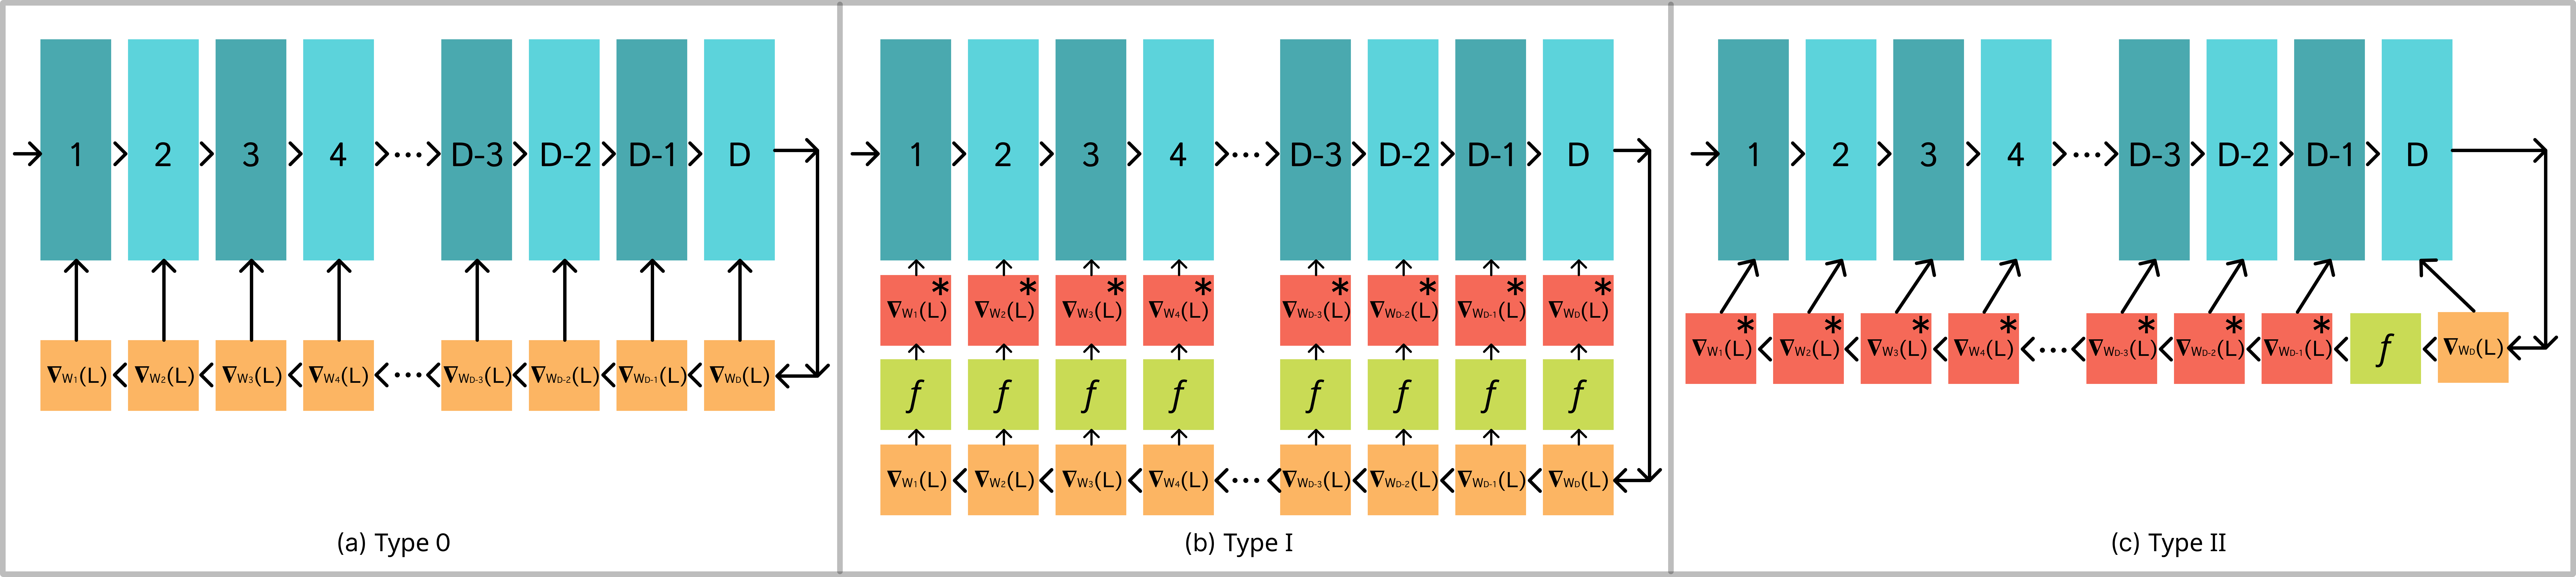
\includegraphics[width=\textwidth]{PGT_Types}
\caption{ Different ways of altering gradients in the backward pass. Blue blocks denote
a different layers. Orange blocks indicate the backward graph with unmodified gradients.
Green blocks represent transformation functions, while red blocks indicate transformed
gradients. }
\label{fig:gradient_altering}
\vspace{-0.5cm}
\end{figure}



\textbf{Type 0:} No modification: In this method, we calculate the gradients using the
standard calculus rules and use the chain rule to calculate the gradients of the rest of
the network's parameters, also known as backpropagation as portrayed in Fig.
\ref{fig:gradient_altering}(a). The network is then updated with the gradient descent
equation:

\begin{equation}
% \hspace{4cm}
W_i^{t+1} = W_i^t - \lambda\ \nabla_{W_i}(L)
\hspace{2cm}
i=D,D-1,\ldots,1
\end{equation}

\textbf{Type I:} Independent gradient modification at multiple points: Here the
gradients are first computed using standard procedure and then individually altered as
shown in Fig. \ref{fig:gradient_altering}(b). Gradient clipping
\cite{pascanu2013difficulty} and Adaptive gradient clipping \cite{brock2021high} are
examples of such modifications. In both of these methods, the gradients are first
computed using standard rules and then they are modified using some function. It can be
described as:

\begin{equation}
% \hspace{4cm}
W_i^{t+1} = W_i^t - \lambda\ f(\nabla_{W_i}(L))
\hspace{2cm}
i=D,D-1,\ldots,1
\end{equation}

where the gradients $\nabla_{W_i}(L)$ are transformed using the transformation function
`$f$' before the weight update.

\textbf{Type II:} Gradient modification at a point very early in the backward graph: In
this type of modification, the gradient is altered at a very early stage in the backward
computation graph and then all subsequent gradients are generated using the values
obtained with the modified gradients. We illustrate this type of modification in Fig.
\ref{fig:gradient_altering}(c). Because of the chain rule, network parameters whose
gradients are connected to the point of alteration in the computation graph also gets
subsequently altered. It can be described as:

\begin{align}
% \hspace{4cm}
W_D^{t+1} &= W_D^t - \lambda\ f(\nabla_{W_D}(L)) & \\
W_i^{t+1} &= W_i^t - \lambda\ \nabla_{W_i}(L)^{*} &\hspace{-1cm} i=D-1,\ldots,1
\end{align}

where the gradient $\nabla_{W_D}(L)$ is first transformed using the transformation
function `$f$' and then this transformed gradient is propagated through the rest of the
backward graph. All other gradient vectors $\nabla_{W_i}(L)^{*}$ are computed as is, but
because of the early injection of the transformed gradient $\nabla_{W_D}(L)$, all other
gradient vectors that are connected to the transformed gradient through the chain rule
($\nabla_{W_i}(L)^{*}$,\ \ i=D-1,\ldots,1), gets subsequently altered.

Type I is computationally more expensive than type II as it requires altering the
gradients of each and every parameter individually. Type II modification recomputes
gradients at each and every location through the natural flow of backpropagation. We
propose PowerGrad Transform (PGT), a type II method that modifies the gradients at the
softmax layer.




The following are the major contributions of this paper:

\begin{enumerate}

\item We propose PowerGrad Transform, which decouples the backward and the forward
passes of neural network training and enables a considerably better fit to the dataset.
PGT is a performance enhancement method that alters the gradients in the backward pass
before the update step leading to accelerated training and a significant boost in the
network's predictive performance.

\item We perform theoretical analysis of the properties of the PowerGrad transformation
and explore its effect on weight parameters and gradients, logits, loss values and class
separation (section \ref{sec:pgt_prop}).

\item We provide complete results from a variety of models (non-BN and BN ResNets,
SE-ResNets) using the ImageNet dataset. We empirically conclude that PGT helps a network
to improve by locating a more optimum convergence point. Additionally, we conduct
ablation studies and compare its effects to those of regularization methods.

\end{enumerate}

\section{Related Works}
\label{sec:Rela}


Gradient Clipping \cite{pascanu2013difficulty} is a gradient modification method that
involves clipping/altering the gradients with respect to a predefined threshold value
during backward propagation through the network and updating the weights using the
clipped gradients \cite{zhang2019gradient}\cite{smith2020generalization}. By rescaling
the gradients, the weight updates are likewise rescaled, significantly reducing the risk
of an overflow or underflow \cite{pascanu2012understanding}. GC can be used for training
networks without batch-normalization. At larger batch sizes, the clipping threshold in
GC becomes highly sensitive and requires extensive finetuning for various models, batch
sizes, and learning rates. As we demonstrate later in our studies, GC is not as
effective in improving the performance of non-normalized networks. Adaptive Gradient
Clipping \cite{brock2021high} is developed to further enhance backward pass gradients
than what is performed by GC. It takes into account the fact that the ratio of the
gradient norm to the weight norm can provide an indication of the expected change in a
single step of optimization. Label smoothing, introduced by Szegedy et al.
\cite{szegedy2016rethinking}, utilizes smoothing of the ground truth labels as a method
to impose regularization on the logits and the weights of the neural network. AGC
performs better than GC in non-normalized networks. However, we show that PGT
outperforms both in networks such as ResNets.

Knowledge distillation (KD) \cite{hinton2015distilling} is a process in which two
networks are trained with hard and soft labels alternatively. Variants of knowledge
distillation include self-distillation \cite{zhang2018deep}, identical student network
distillation \cite{furlanello2018born}, channel distillation \cite{ge2019distilling},
regularizing wrong predictions \cite{yun2020regularizing} and representation or
embedding based knowledge distillation \cite{yao2018deep}. Even though both PGT and KD
requires probability manipulation, the key difference is that in the latter the
transformation is applied in the forward pass, while PGT is a backward pass modification
only. In distillation settings the temperature parameter is a part of the network's
computation graph. In the case of PowerGrad Transform, we directly tamper the gradients
without introducing any change in the forward pass. PGT differs from self-knowledge
distillation as it neither introduces any additional sub-modules nor creates different
ensembles to improve the performance of the model. PGT follows the standard neural
network training mechanism with modified gradients.

\section{PowerGrad Transform}
\label{sec:Powe}


\begin{figure}[t]
\centering
\begin{subfigure}{.5\textwidth}
\centering
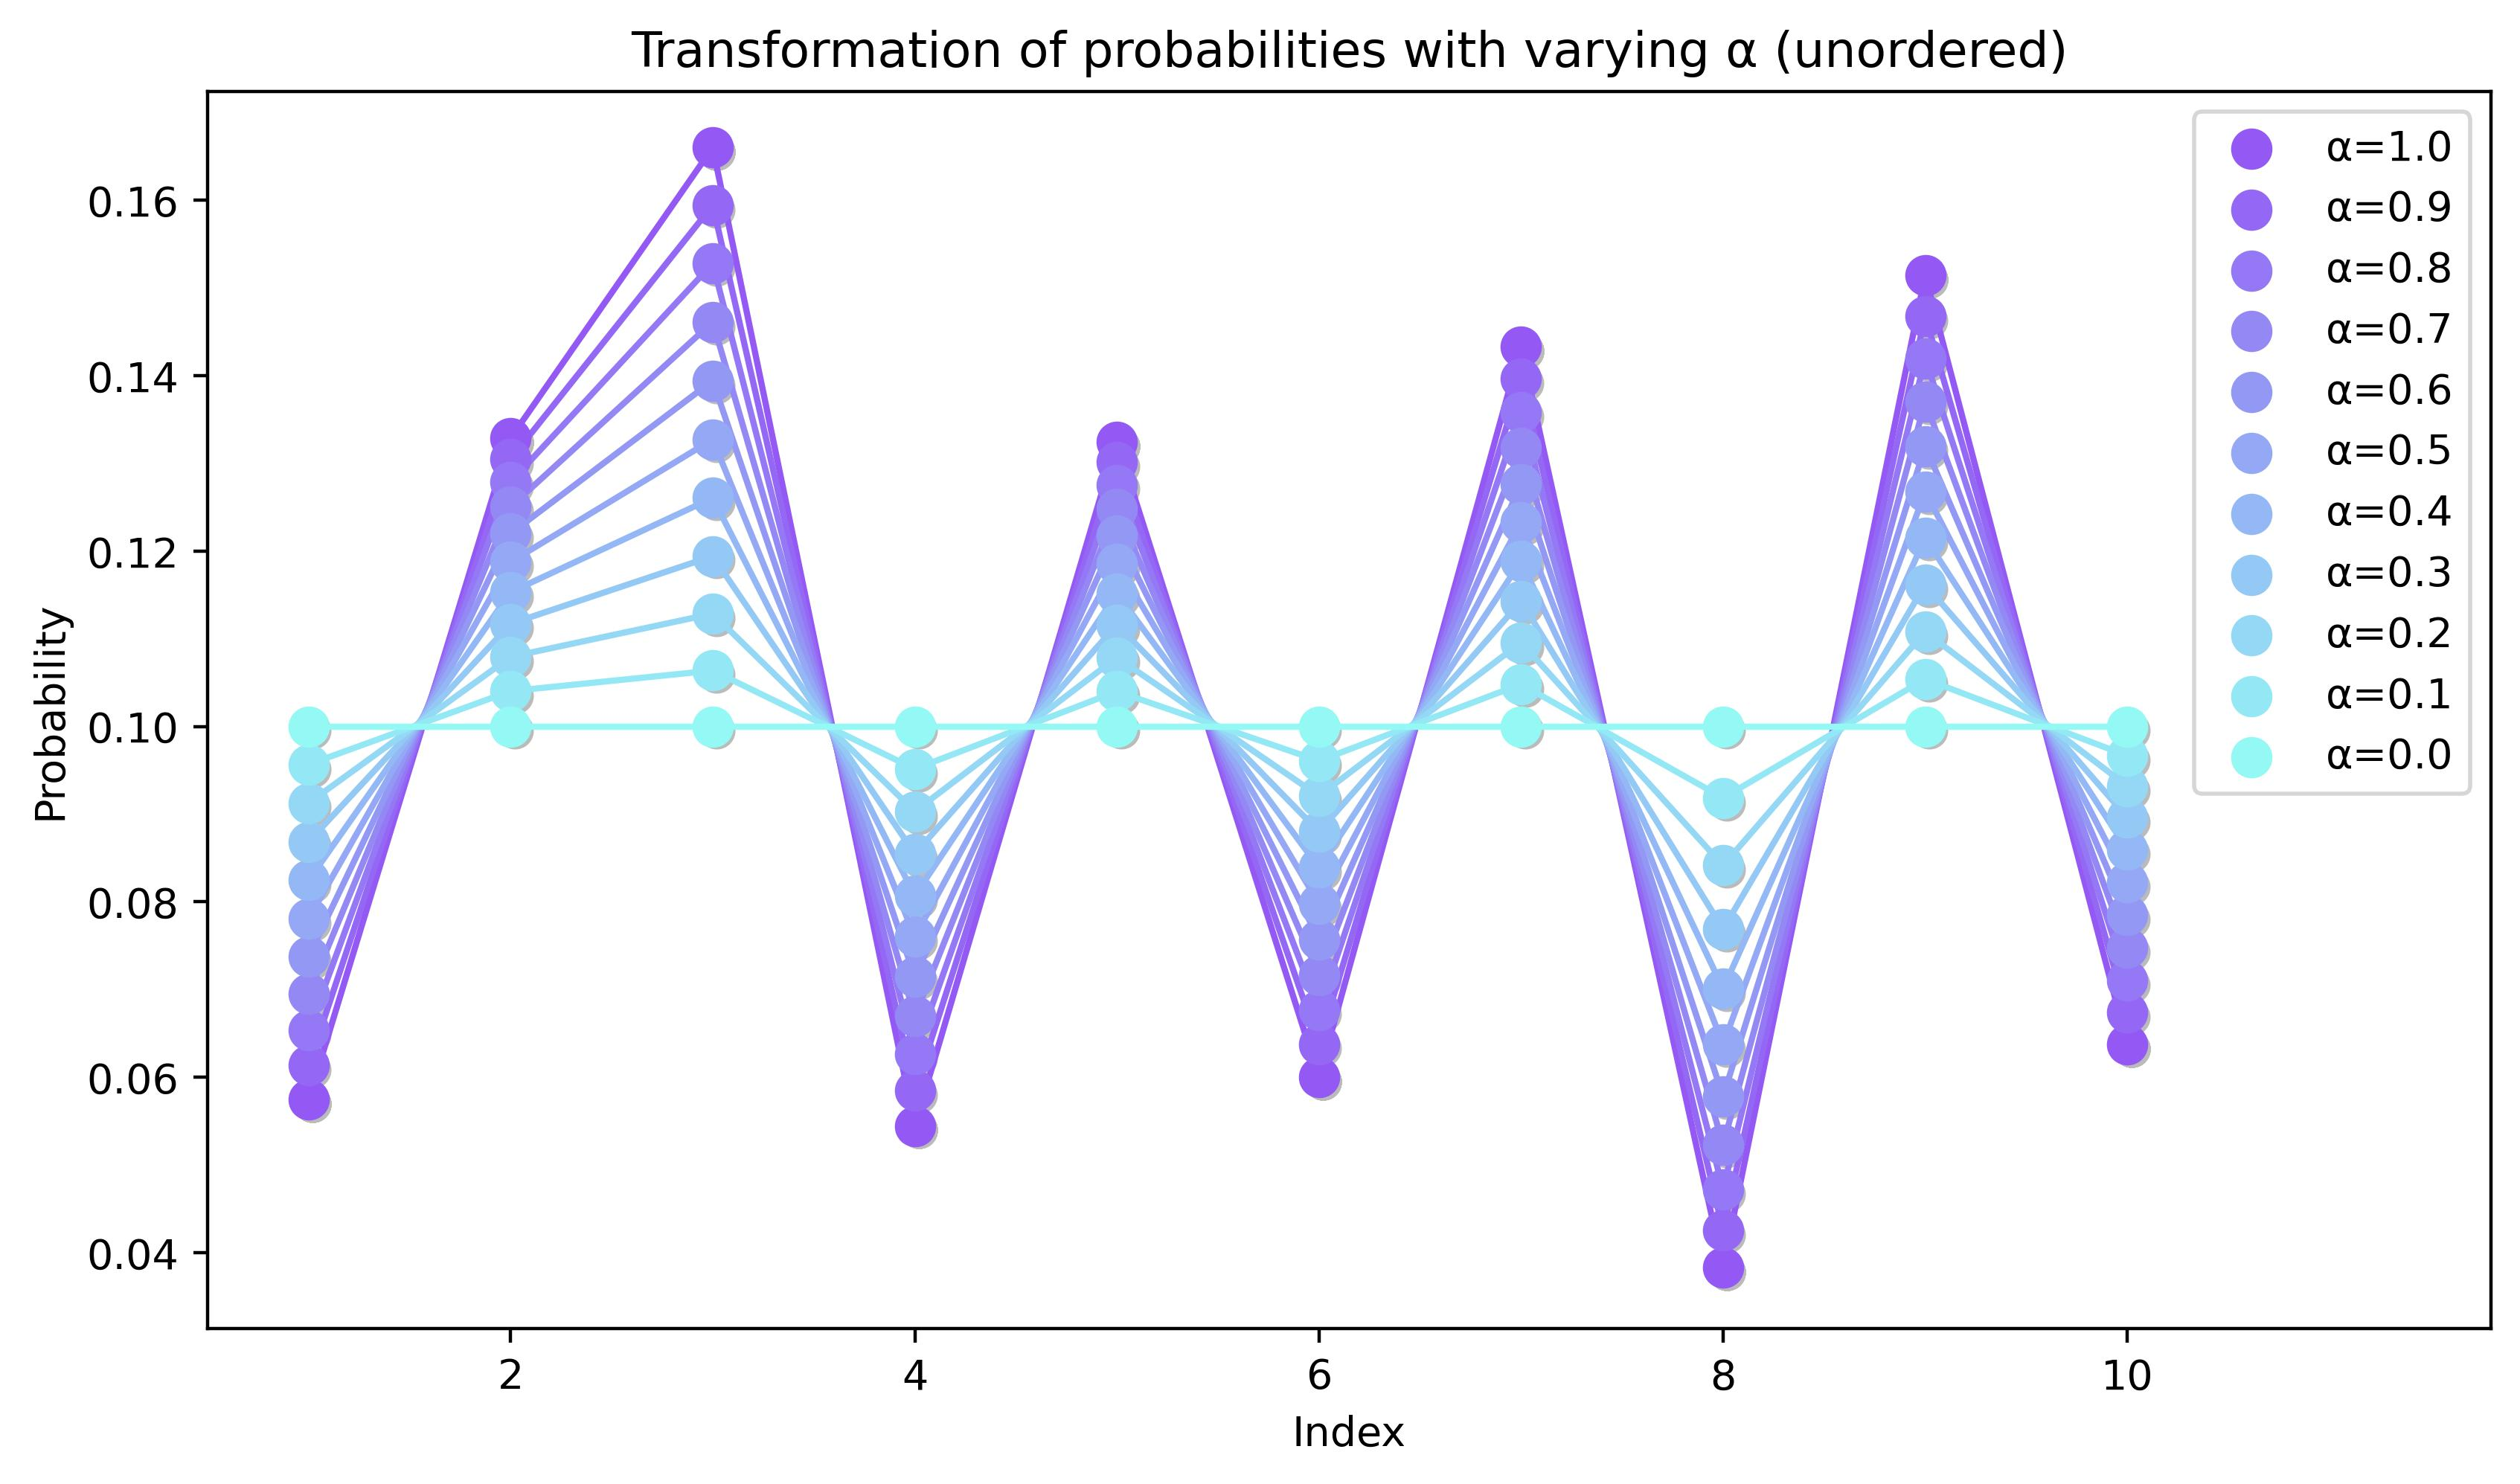
\includegraphics[width=0.98\textwidth]{prob_transform_unordered}
\caption{Unordered distribution}
\end{subfigure}%
\begin{subfigure}{.5\textwidth}
\centering
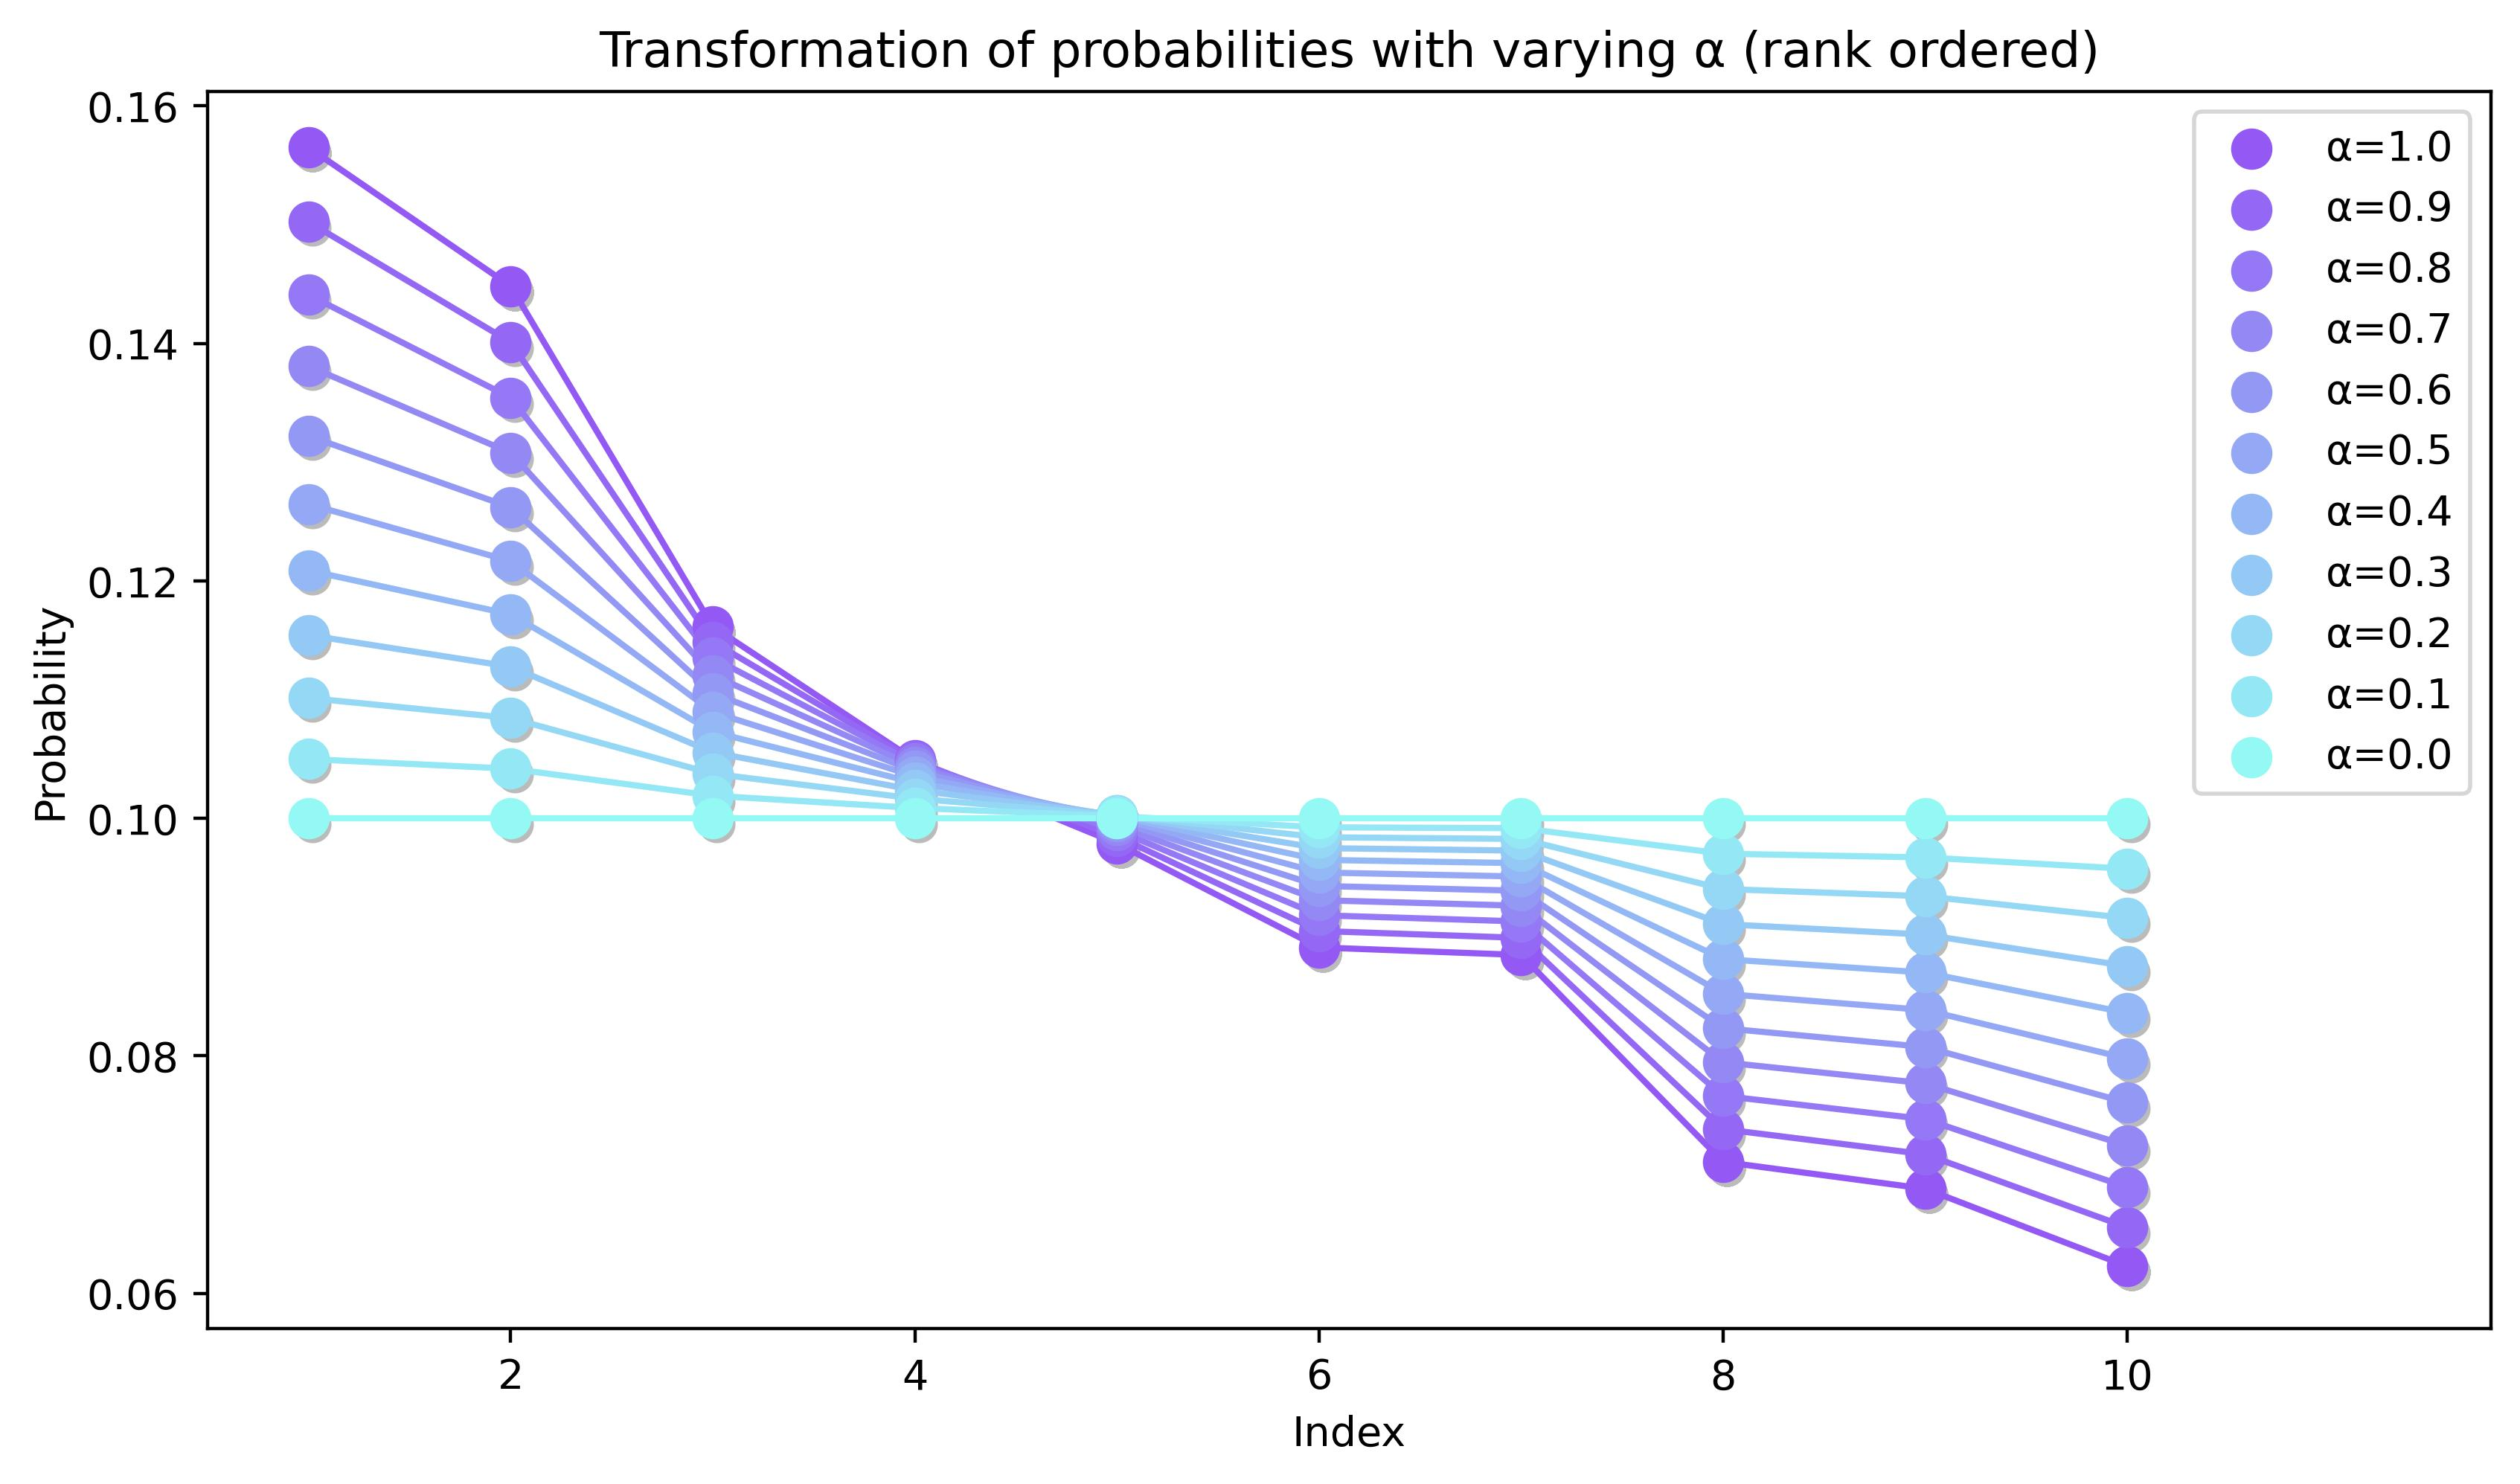
\includegraphics[width=0.98\textwidth]{prob_transform_ordered}
\caption{Rank ordered distribution}
\end{subfigure}
\caption{ Illustration of the impact of PowerGrad Transform on probability values of an
arbitrary distribution (number of classes, $C=10$). $\alpha=1$ indicates the unmodified
distribution. As $\alpha$ reduces from $1$ to $0$, the probability distributions (left:
unordered or right: ordered) becomes flatter and flatter, approaching the uniform
distribution of $1/C$ for every index. }
\label{fig:prob_plots}
\vspace{-0.5cm}
\end{figure}


A neural network with parameters $W$ generates $C$ logits denoted by $z$ for every input
vector $x$. $z$ is given as $z=Wx$. Then a set of probability values $p_i$ are generated
from the logits using a softmax function which is defined as $p_i=\frac{e^{z_i}}{\sum
_{j=1}^C e^{z_j}}$. $p_i$ and $z_i$ represent the predicted probability values and the
logits for the $i^{th}$ class respectively. Following this step, the loss function is
invoked and the loss between the predicted probability values the ground truth labels
(which is also a probability distribution) is calculated. If the loss function is
cross-entropy loss, then the value of the loss is given as $L=-\sum _{i=1}^C q_i \log
\left(p_i\right)$ where $q_i$ is the ground truth label of the $i^{th}$ class for a
particular training example. By standard gradient update rule, we can calculate the
gradient of the loss with respect to the logits which takes the form $\frac{\partial
L}{\partial z_i}=p_i-q_i$.

The PowerGrad Transform technique is now described. We introduce a hyperparameter
$\alpha$, which takes a value between $[0, 1]$ and regulates the degree of gradient
modification. Fig. \ref{fig:prob_plots} shows the effects of the transform under
different values of $\alpha$ for different distributions. The PowerGrad Transform method
modifies the predicted probability values in the backward pass as follows:

\vspace{-0.5cm}
\begin{equation} \hspace*{3.5cm} p_i'=\frac{p_i^{\alpha }}{\sum _{j=1}^C
p_j^\alpha} \ \ \ \ \ \ \ \ i=1,\dots,C\ \ \ \ \ 0 \leq \alpha\leq 1
\label{transformed_probabilities} \end{equation}

The above transformation changes the gradient of the loss with respect to the logits as
follows:

\vspace{-0.5cm}
\begin{equation} \widehat{\frac{\partial L}{\partial z_i}}=p_i'-q_i
\label{PGT_logit_derivative}
\end{equation}

The rest of the backward pass proceeds as usual. We denote the original probability
distribution as $P$ (with values $p_i$ at the $i^{th}$ index) and the transformed
distribution as $P'$ (with values $p_i'$ at the $i^{th}$ index).



\subsection{Properties of the PowerGrad transformation}
\label{sec:pgt_prop}

We use the same setup as described in section \ref{sec:Powe}. To explore the properties
of PGT, we start by investigating the effect of the transform on the softmax
probabilities.

\textbf{Lemma 1.} For any arbitrary probability distribution $P$ with probability values
given by $p_i$ for $i=1,\dots,C$, the corresponding transformed probability values
$p_i'$ given by [Eq. \ref{transformed_probabilities}] has a threshold $\Big(\sum
_{j=1}^C p_j^{\alpha}\Big)^{\frac{1}{\alpha-1}}$ and

\vspace{-0.5cm}
\begin{equation} \begin{split} p_i' \geq p_i & \text{,\ \ if } p_i \leq
\Big(\sum _{j=1}^C p_j^{\alpha }\Big)^{\frac{1}{\alpha-1}} \\ \hspace*{1cm}
p_i' < p_i & \text{,\ \ if } p_i > \Big(\sum _{j=1}^C
p_j^{\alpha}\Big)^{\frac{1}{\alpha-1}} \end{split} \label{eqn:threshold0}
\end{equation}

\vspace{-0.2cm}
We call this threshold, the \textit{stationary threshold}. The stationary threshold is
that value of $p_i$ that does not change after the transformation. Therefore, when $p_i$
is greater than the \textit{stationary threshold}, $p_i' < p_i$.



\textbf{Proposition 1.} At $\alpha=0$, the stationary threshold equals $1/C$ and all
values of the transformed distribution $p_i'$ reduces reduces to the uniform
distribution for $i=1,\dots,C$,.

We have established that values of $p_i$ which are greater than the stationary threshold
decreases and move down towards the stationary threshold, and values in $p_i$ lower than
the stationary threshold moves up towards the stationary threshold. Therefore, this
transformation makes the distribution more uniform (i.e. it smooths out the actual
distribution) as $\alpha$ is decreased from $1$ and down towards $0$. This final
observation in the following theorem.



\textbf{Theorem 1.} For any arbitrary probability distribution $P$ with probability
values $p_i$ for $i=1,\dots,C$, the stationary threshold of the transformed distribution
$P'$ with probability values $p_i'=\frac{p_i^{\alpha}}{\sum _{j=1}^C p_j^\alpha}, 0 \leq
\alpha \leq 1$ is a monotonically non-decreasing function with respect to $\alpha$.



We provide the proofs in supplementary section \ref{sec:proofs} and conclude that the
stationary threshold is a monotonic non-decreasing function with respect to $\alpha$.
Also the derivative of PGT function with respect to the true probabilities is
non-negative which in turn means that the transformation is an order-preserving map. All
values greater than the threshold move towards the threshold after transformation and
all values below the threshold also move towards the threshold, and the threshold itself
moves monotonically towards $1/C$ as $\alpha$ is decreased from $1$ to $0$. This
concludes that the transformation smooths the original distribution.





\begin{figure}[!t]
\centering
\begin{subfigure}{.33\textwidth}
\centering
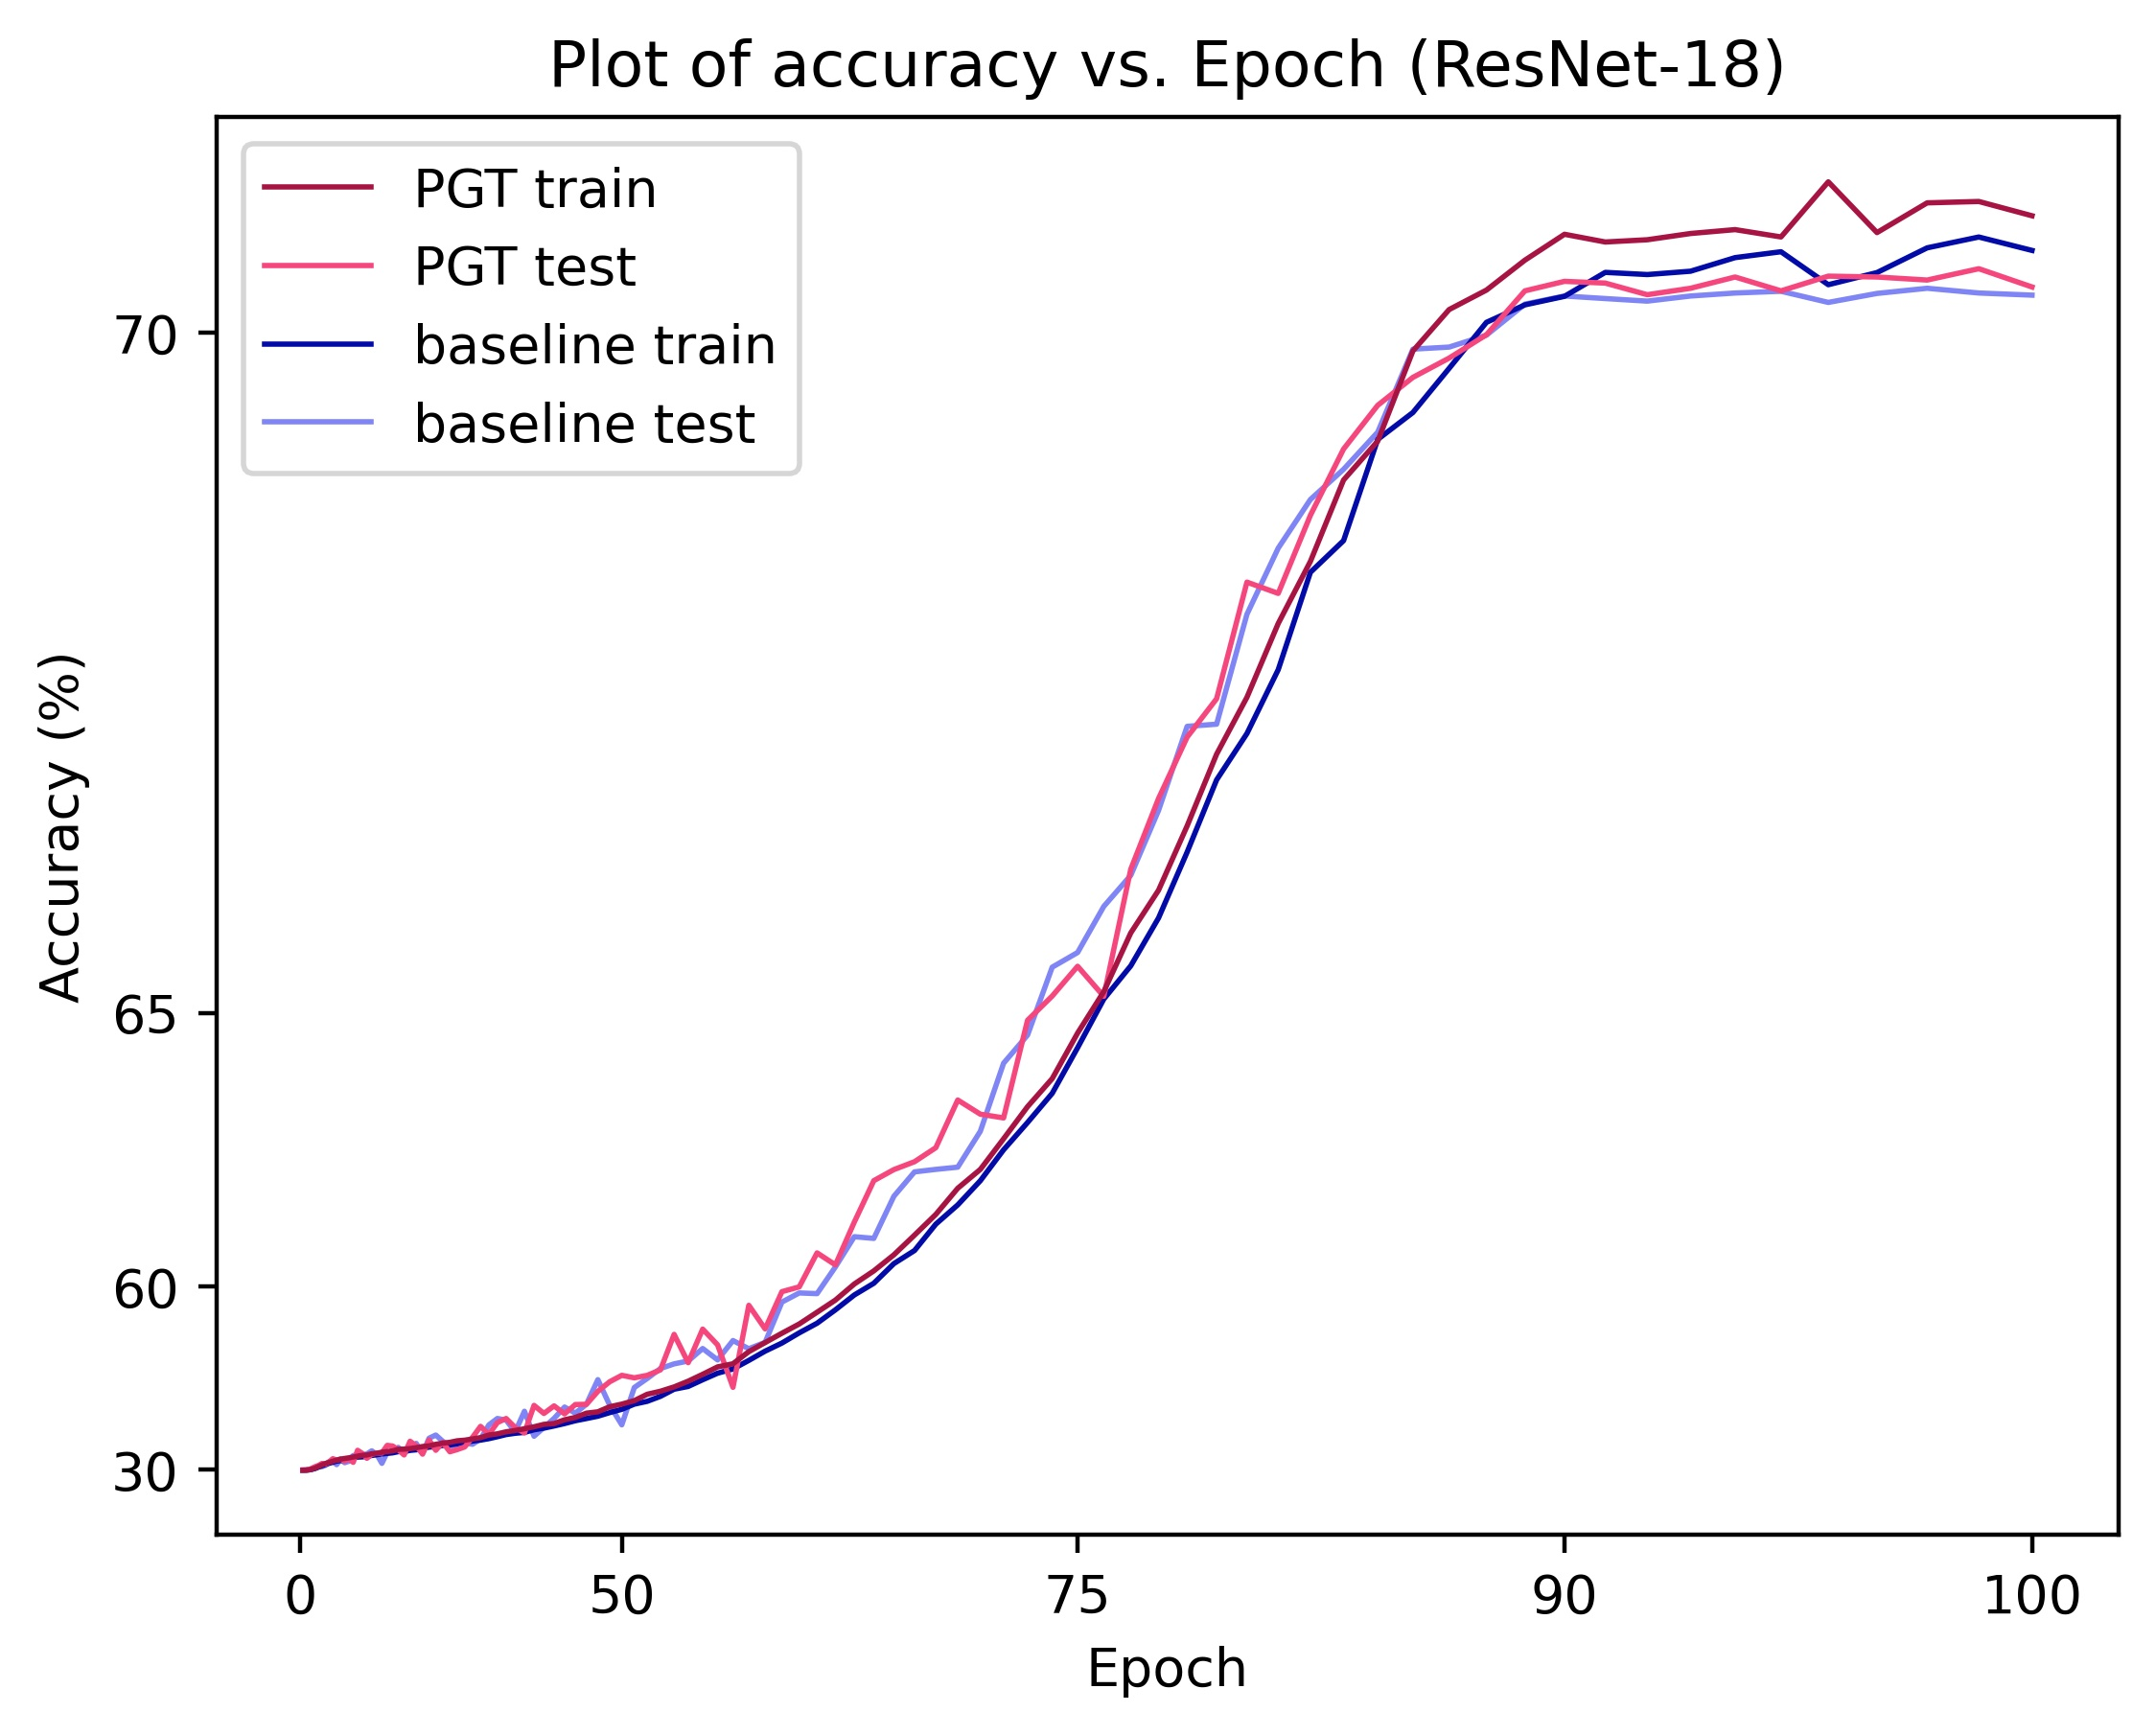
\includegraphics[width=0.98\textwidth]{acc_vs_epoch_r18}
\caption{Plot of training and test accuracies (ResNet-18)}
\end{subfigure}%
\begin{subfigure}{.33\textwidth}
\centering
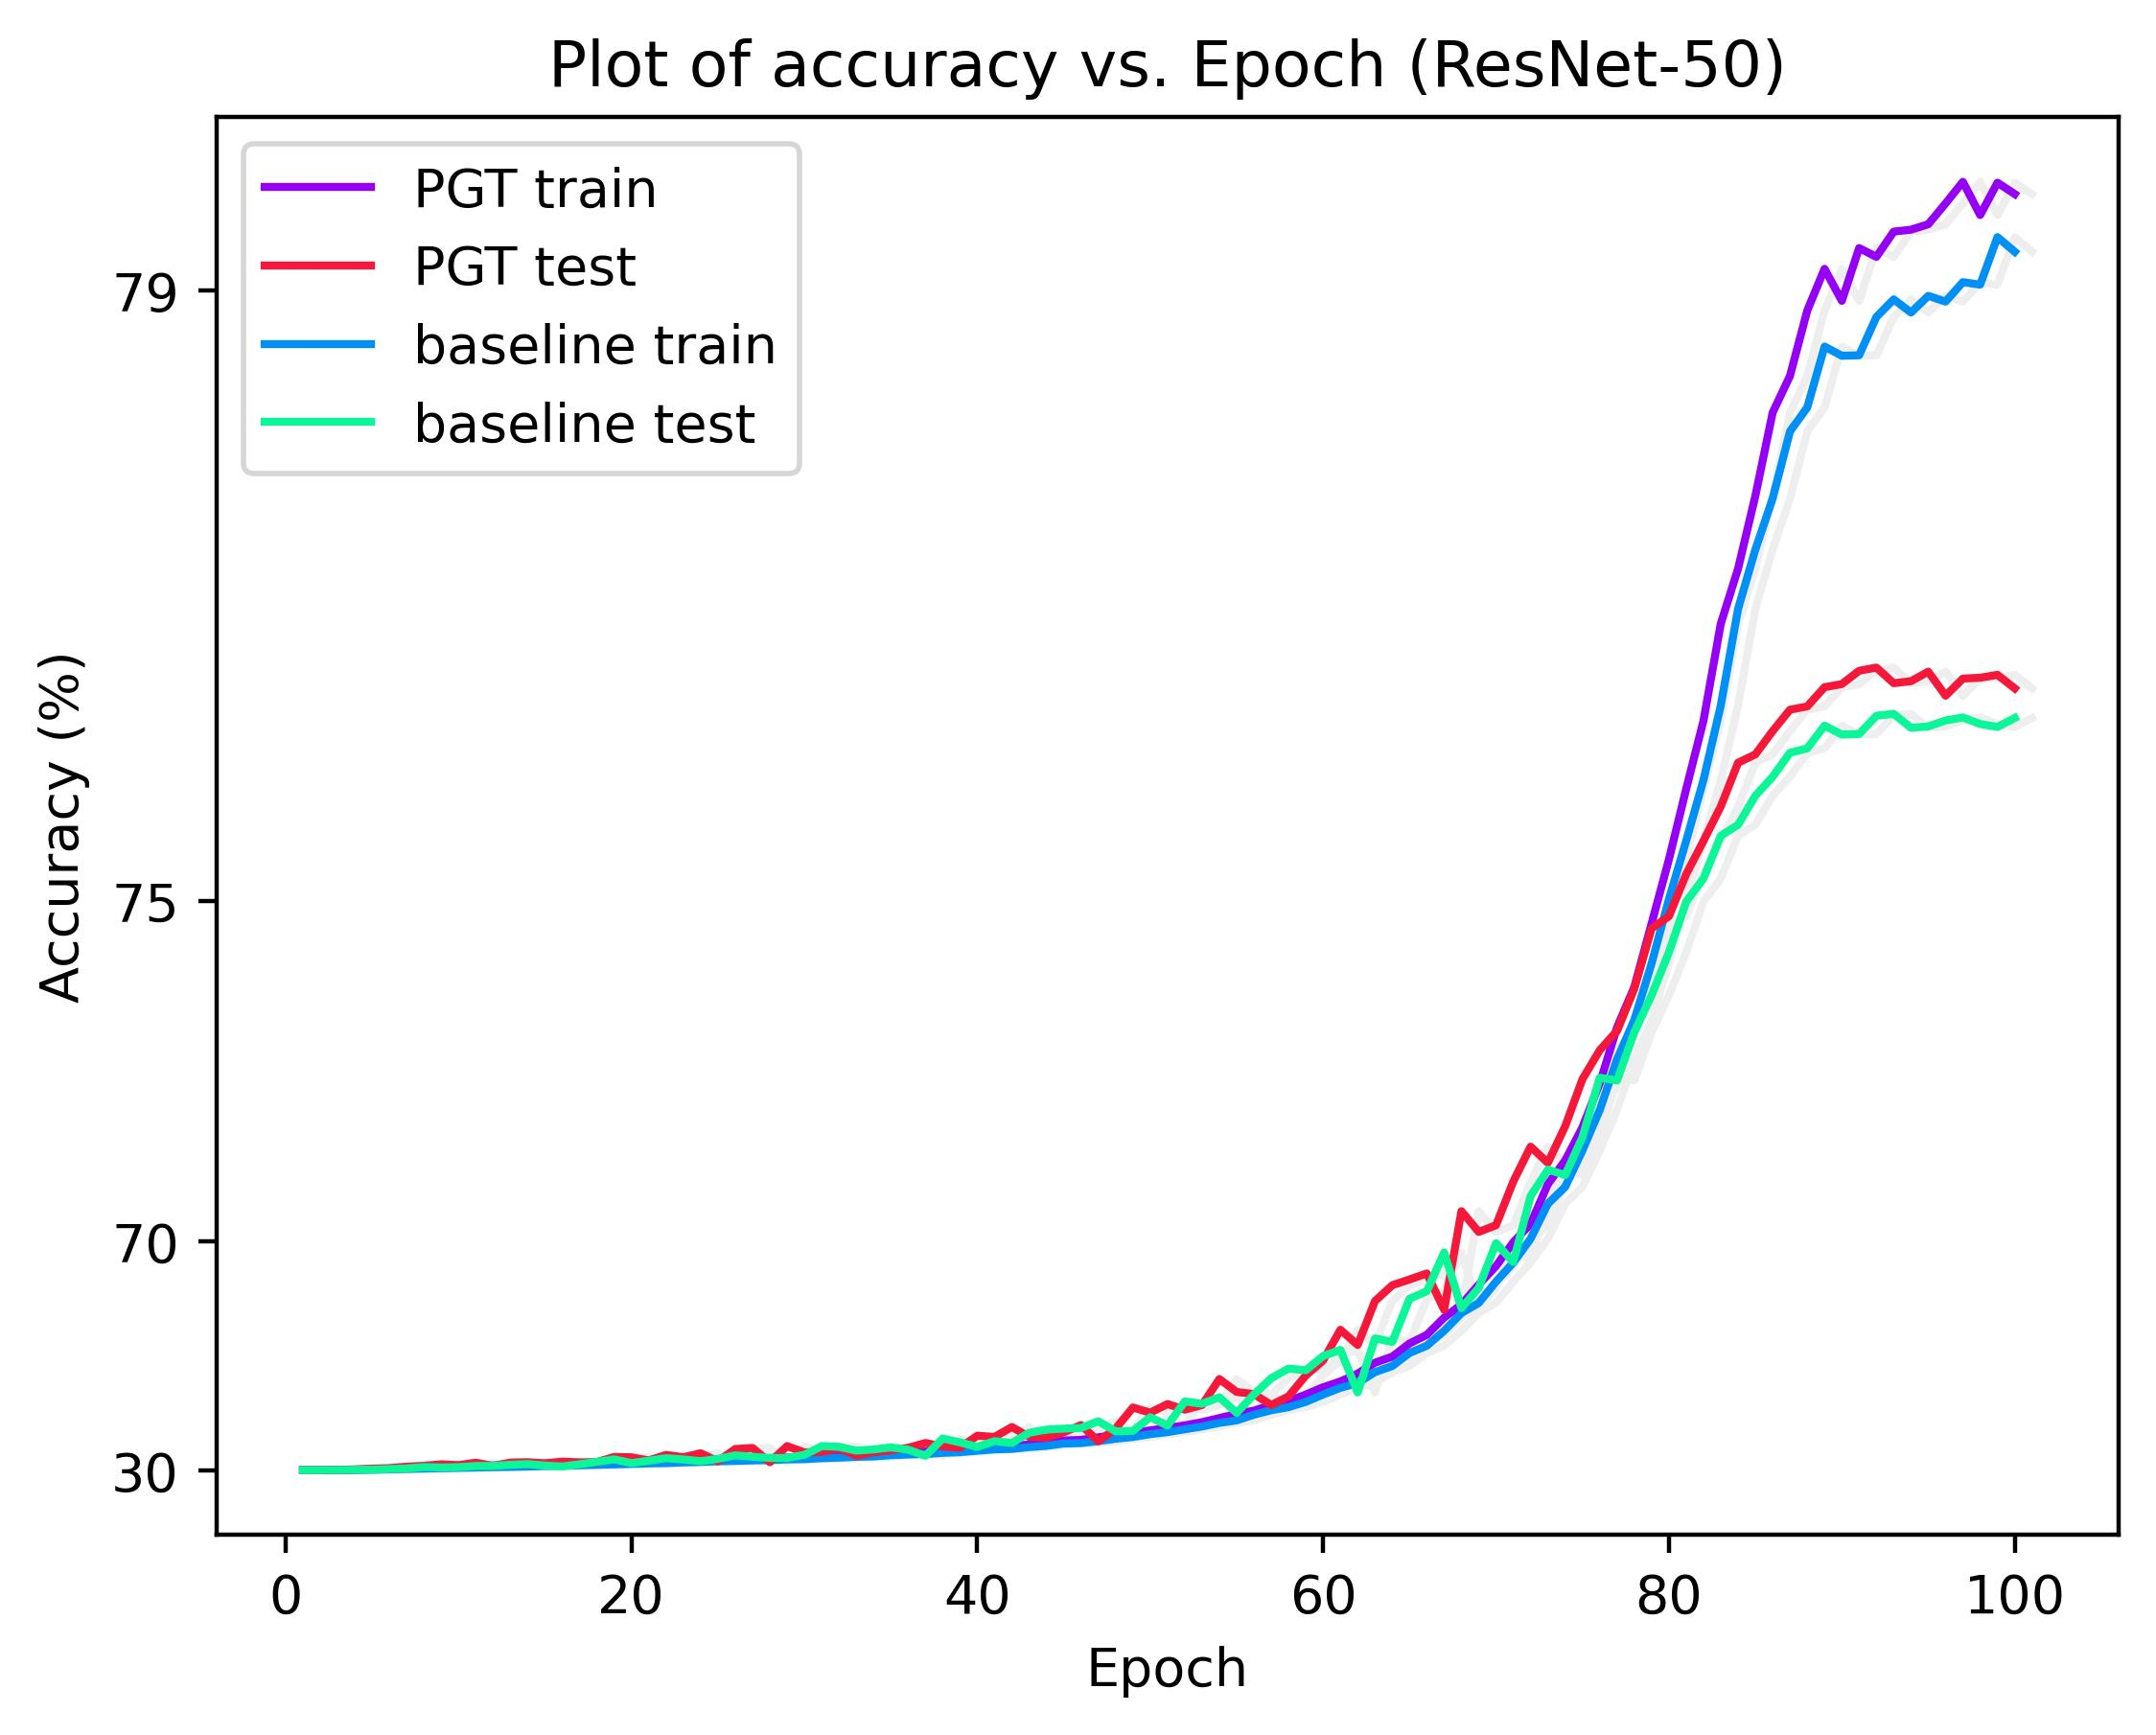
\includegraphics[width=0.98\textwidth]{acc_vs_epoch_r50}
\caption{Plot of training and test accuracies (ResNet-50)}
\end{subfigure}%
\begin{subfigure}{.33\textwidth}
\centering
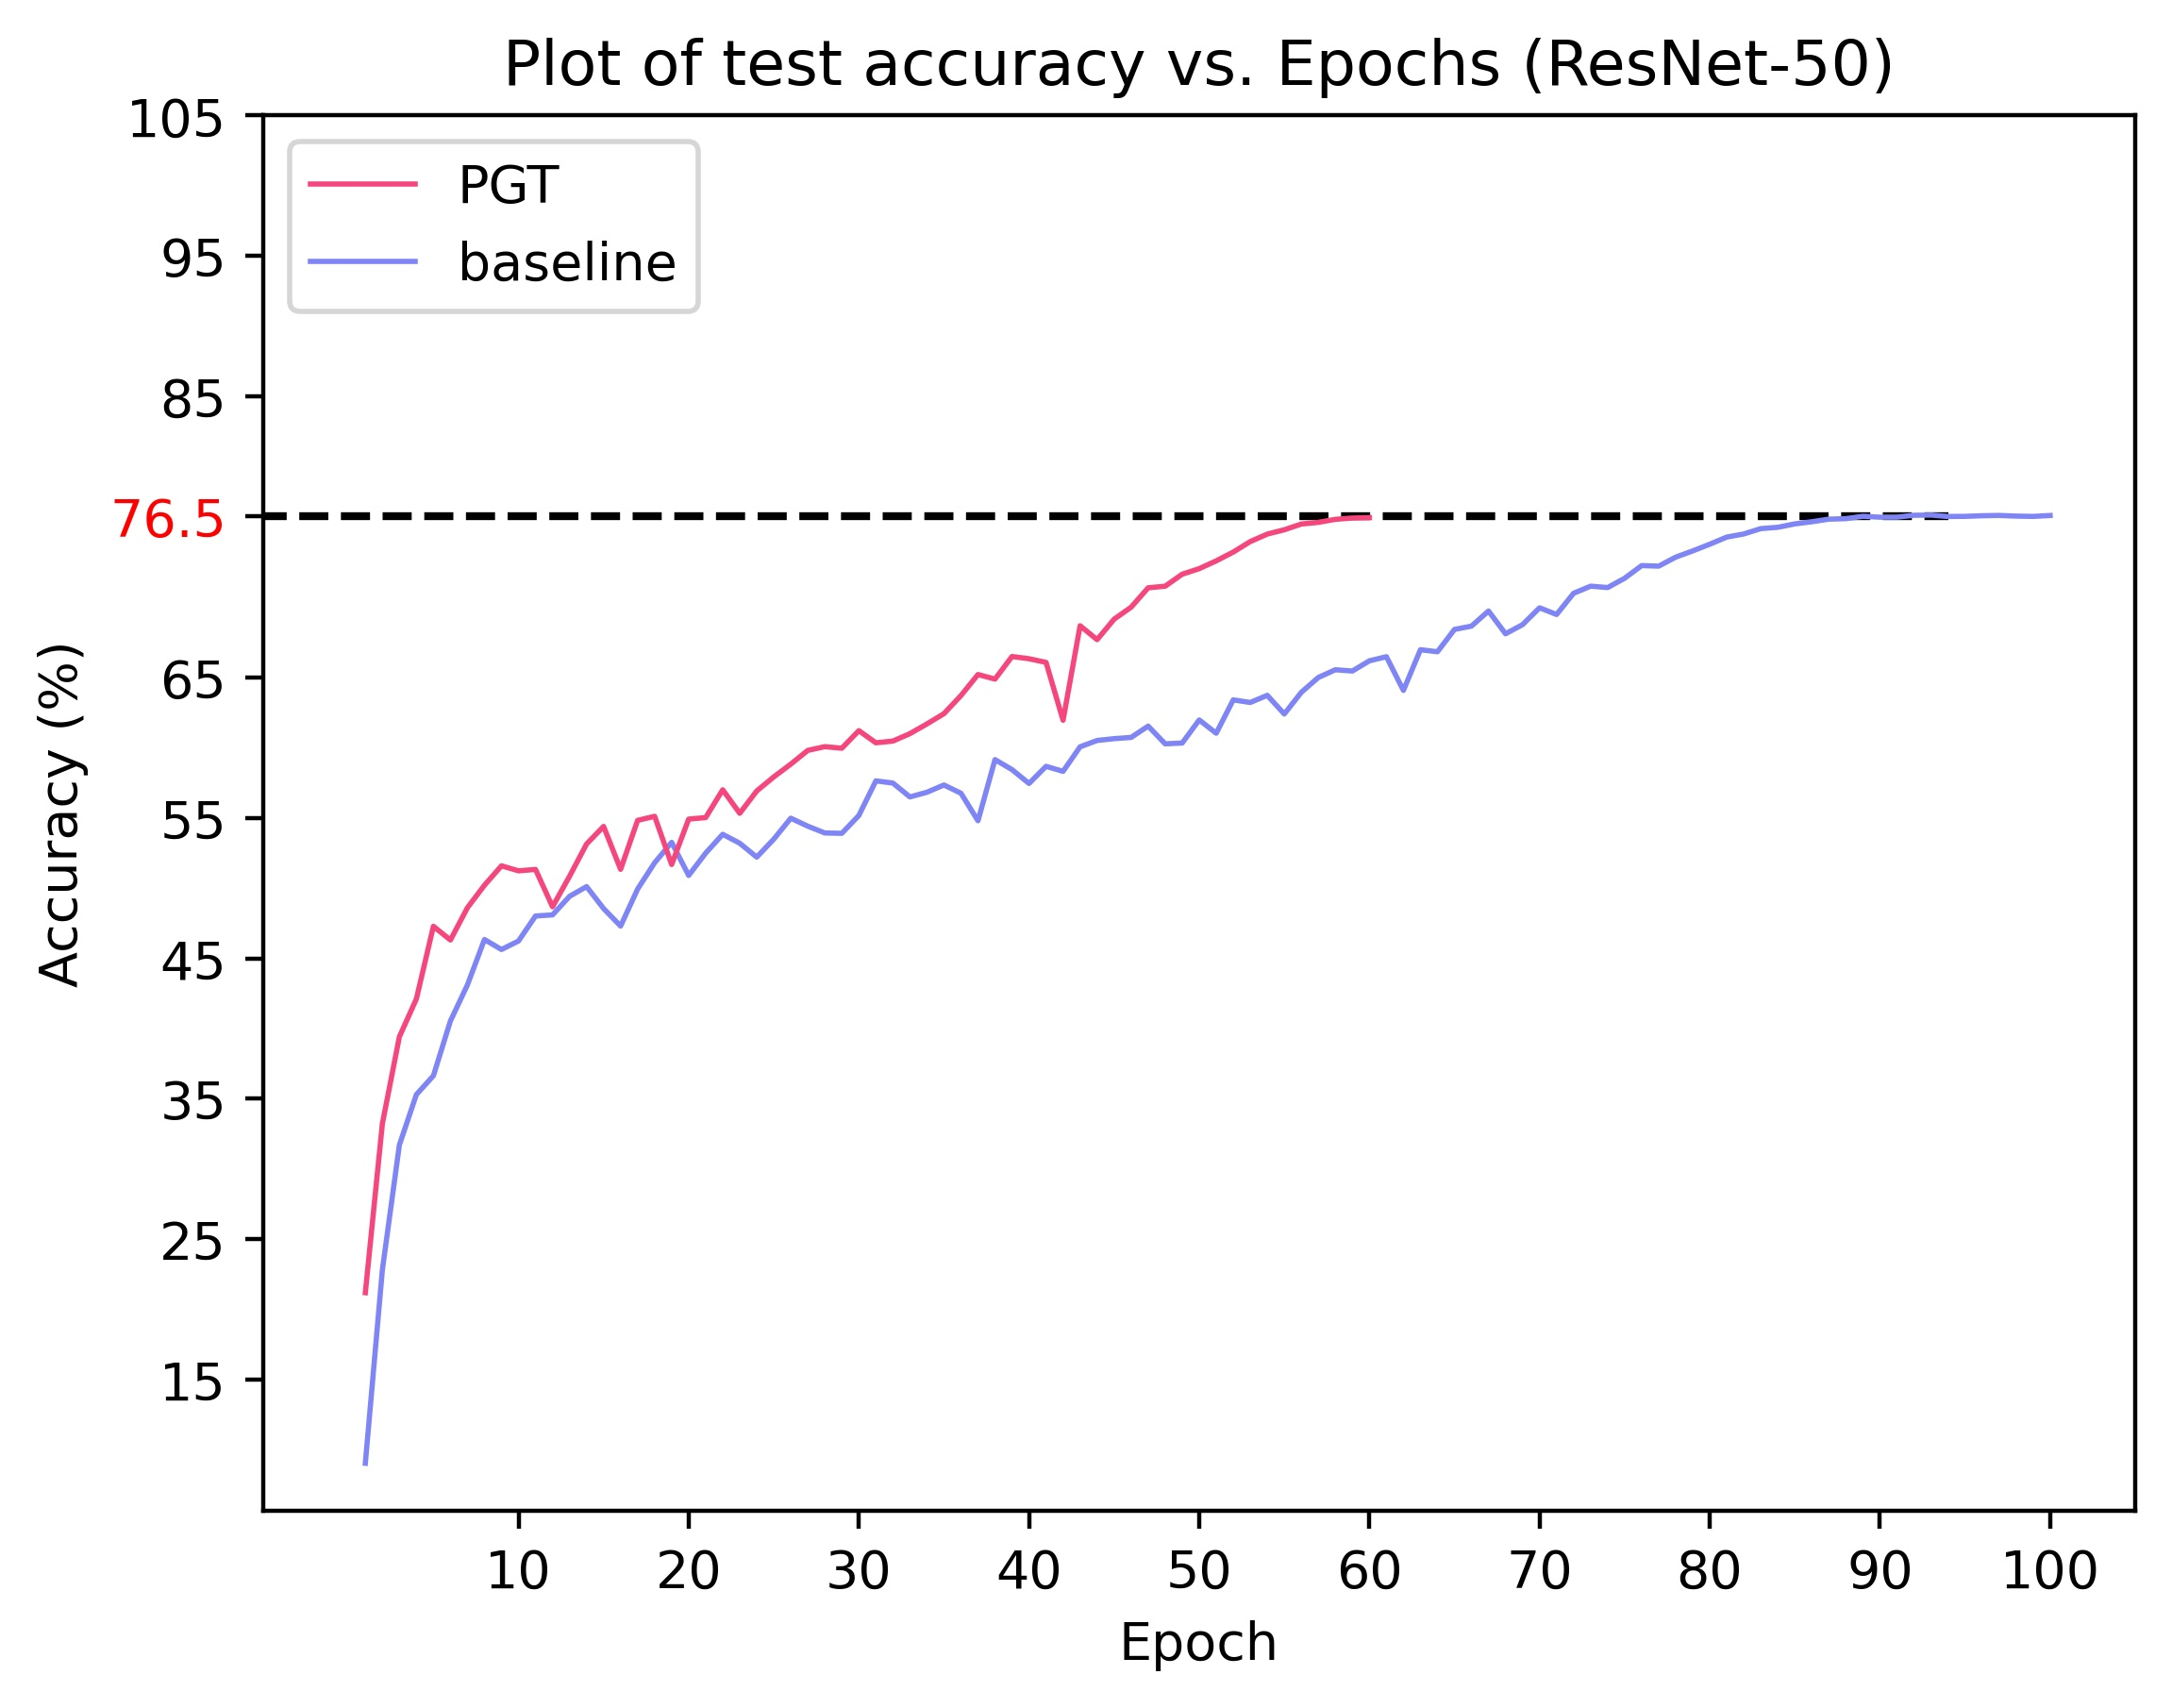
\includegraphics[width=0.98\textwidth]{acc_vs_epoch_r50_60epochs}
\caption{Plot of test accuracies (ResNet-50)}
\end{subfigure}
\caption{ Log-log plots of training and test accuracies and comparison with baseline of
batch-normalized variants: \textbf{(a)} ResNet-18 ($\alpha=0.25$), \textbf{(b)}
ResNet-50 ($\alpha=0.3$). \textbf{(c)} Training speed comparison between PGT ($60$
epochs) and baseline ($100$ epochs). They both converge to the same test accuracy
($76.5\%$) on ImageNet-1K. PGT's accelerated training saves $40\%$ of the epoch budget.
}
\label{fig:metrics}
\vspace{-0.5cm}
\end{figure}



PGT, other than having the properties mentioned above, also satisfies the following. The
transformation:
\begin{enumerate}
\item restricts the magnitude of the directional derivative for each logit from becoming too small or too high
\item enhances gradient behavior of weights in a manner that improves learning
\item leads to better class separation.
\end{enumerate}

We demonstrate each of these effects in detail in supplementary sections
\ref{sec:pgt_logit_derivative}, \ref{sec:pgt_weight_gradients} and
\ref{sec:pgt_class_separation} respectively.

\section{Experiments}
\label{sec:Expe}




We perform experiments on different variants ResNets using the ImageNet-1K dataset
\cite{deng2009imagenet}. All models are trained on four V100 GPUs with a batch size of
$1024$. We utilize a common set of hyperparameters for all experiments, which are as
follows: 100 epoch budget, 5 epochs linear warmup phase beginning with a learning rate
of $4\times 10^{-4}$ and ending with a peak learning rate of $0.4$, a momentum of $0.9$
and weight decay of $5\times 10^{-4}$, the SGD Nesterov optimizer and mixed precision.
In our studies, we employ either a step scheduler (dividing the learning rate by $10$ at
the $30^{th}$, $60^{th}$, and $90^{th}$ epochs) or a cosine decay scheduler
\cite{loshchilov2016sgdr}. We find $\alpha=0.25$ and $\alpha=0.05$ to be good choices
for ResNet-18 and ResNet-50, though larger values such as $\alpha=0.3$ also have good
performance as well. The experimental results are shown in Table
\ref{tab:imagenet_table}, and we mention the value of the PGT hyperparmeter ($\alpha$)
in each experiment. We explore different values of $\alpha$ in section \ref{sec:Abla}
and provide detailed grid plots in the supplementary section\footnote{Reproducible code,
training recipes for the experiments, pretrained checkpoints and training logs are
provided at: \url{ https://github.com/skalien/power-grad-transform }.}.




\begin{table}[!t]
\centering
\caption{ Results and comparison table for networks trained on ImageNet-1K. Best
training and test accuracies are highlighted in red and blue respectively. Accuracy
differences are highlighted in yellow. }
\label{tab:imagenet_table}
\begin{tabular}{cccccccc}
\multirow{2}{*}{\textbf{Model}} & \multirow{2}{*}{\textbf{Scheduler}} &
\multirow{2}{*}{\textbf{Method}} & \textbf{PGT} & \textbf{Train}
& \textbf{Train} & \textbf{Test} & \textbf{Test} \\
& & & \textbf{($\alpha$)} & \textbf{Acc.(\%)} & \textbf{Diff(\%)} &
\textbf{Acc.(\%)} & \textbf{Diff(\%)} \\
\midrule
\multirow{2}{*}{SE-ResNet-50} & \multirow{2}{*}{Cosine} & Baseline & - & 81.5 &
\textcolor{olive}{\multirow{2}{*}{\textbf{+0.97}}} & 77.218 &
\textcolor{olive}{\multirow{2}{*}{\textbf{+0.734}}} \\
& & PGT & 0.3 & \textcolor{red}{\textbf{82.47}} & & \textcolor{blue}{\textbf{77.952}} &
\\
\midrule
\multirow{2}{*}{ResNet-50} & \multirow{2}{*}{Cosine} & Baseline & - & 79.18 &
\textcolor{olive}{\multirow{2}{*}{\textbf{+0.5}}} & 76.56 &
\textcolor{olive}{\multirow{2}{*}{\textbf{+0.656}}} \\
& & PGT & 0.05 & \textcolor{red}{\textbf{79.68}} & & \textcolor{blue}{\textbf{77.216}} &
\\
\midrule
\multirow{2}{*}{ResNet-50} & \multirow{2}{*}{Step} & Baseline & - & 78.99 &
\textcolor{olive}{\multirow{2}{*}{\textbf{+0.57}}} & 75.97 &
\textcolor{olive}{\multirow{2}{*}{\textbf{+0.524}}} \\
& & PGT & 0.05 & \textcolor{red}{\textbf{79.56}} & & \textcolor{blue}{\textbf{76.494}} &
\\
\midrule
\multirow{2}{*}{ResNet-101} & \multirow{2}{*}{Cosine} & Baseline & - & 82.29 &
\textcolor{olive}{\multirow{2}{*}{\textbf{+0.81}}} & 77.896 &
\textcolor{olive}{\multirow{2}{*}{\textbf{+0.362}}} \\
& & PGT & 0.3 & \textcolor{red}{\textbf{83.1}} & & \textcolor{blue}{\textbf{78.258}} &
\\
\midrule
\multirow{2}{*}{SE-ResNet-18} & \multirow{2}{*}{Cosine} & Baseline & - & 71.42 &
\textcolor{olive}{\multirow{2}{*}{\textbf{+0.18}}} & 71.09 &
\textcolor{olive}{\multirow{2}{*}{\textbf{+0.346}}} \\
& & PGT & 0.25 & \textcolor{red}{\textbf{71.6}} & & \textcolor{blue}{\textbf{71.436}} &
\\
\midrule
\multirow{2}{*}{ResNet-18} & \multirow{2}{*}{Step} & Baseline & - & 69.95 &
\textcolor{olive}{\multirow{2}{*}{\textbf{+0.35}}} & 69.704 &
\textcolor{olive}{\multirow{2}{*}{\textbf{+0.14}}} \\
& & PGT & 0.25 & \textcolor{red}{\textbf{70.3}} & & \textcolor{blue}{\textbf{69.844}} &
\\
\midrule
\multirow{2}{*}{ResNet-18} & \multirow{2}{*}{Cosine} & Baseline & - & 70.38 &
\textcolor{olive}{\multirow{2}{*}{\textbf{+0.15}}} & 70.208 &
\textcolor{olive}{\multirow{2}{*}{\textbf{+0.09}}} \\
& & PGT & 0.25 & \textcolor{red}{\textbf{70.53}} & & \textcolor{blue}{\textbf{70.298}} &
\\
\end{tabular}
\vspace{-0.5cm}
\end{table}





In our experiments with Squeeze-and-Excitation variant of ResNet-50 i.e.
SE-ResNet-50\cite{hu2018squeeze}, we observe significant improvements; a $0.97\%$ boost
in training accuracy and a $0.734\%$ increase in test accuracy. In our experiments with
ResNet-50, we find an increase of $0.5\%$ and $0.656\%$ performance enhancement over the
cosine scheduler baseline for training and testing respectively. The corresponding
improvement over the step scheduler baseline for ResNet-50 is $0.57\%$ (training) and
$0.524\%$ (testing). ResNet-101 sees a higher improvement in training fit, $0.81\%$ to
be exact, while the improvement over the test set is $0.362\%$. Smaller networks such as
SE-ResNet-18 and ResNet-18 sees accuracy boosts which are smaller but nevertheless
positive. With consistent improvements in training accuracies across all cases, we
conclude PGT helps networks learn better representations and arrive at better optimas
during convergence. Per epoch training and test accuracy plots of ResNet-18 and
ResNet-50 (both with and without PGT) are shown in Fig. \ref{fig:metrics}(a,b).
Practioners can also choose to accelerate training and save as much as $40\%$ of the
epoch budget [Fig. \ref{fig:metrics}(c)].

\subsection{Empirical studies on networks without Batch Normalization}
\label{sec:Empi}




We examine issues that occur in non-normalized networks (networks without BN layers). We
use ResNet-18 \cite{he2016deep} as the foundation model trained on ImageNet-1K
\cite{russakovsky2015imagenet}. Deeper networks such as ResNet-34 and ResNet-50 are
impossible to train without Batch Normalization courtesy of the increased depth and so
we solely focus on ResNet-18. We designate different layers with their corresponding
layer indices. Throughout the training process, we monitor variations in the the
per-filter L2-norm of each layer's weights (layer indices are mentioned in section
\ref{sec:r18_layers}). In Fig. \ref{fig:norm_plots}(a), some filters of layer $11$
achieve a norm of zero during training. We refer to this event as `Zeroing Out', and it
occurs when one of the channels (or filters) of a weight tensor gets fully filled with
zeros and such filters do not contribute at all to determine the input-output
relationship of a dataset, as the feature tensor it produces is also filled with zeros
for the corresponding filter. When a filter once zeroes out, it does not recover with
further training, as all gradients that it receives in future iterations are all zeros. 



\begin{figure}[t]
\centering
\captionsetup{font=footnotesize}

\begin{subfigure}[t]{0.16\textwidth}
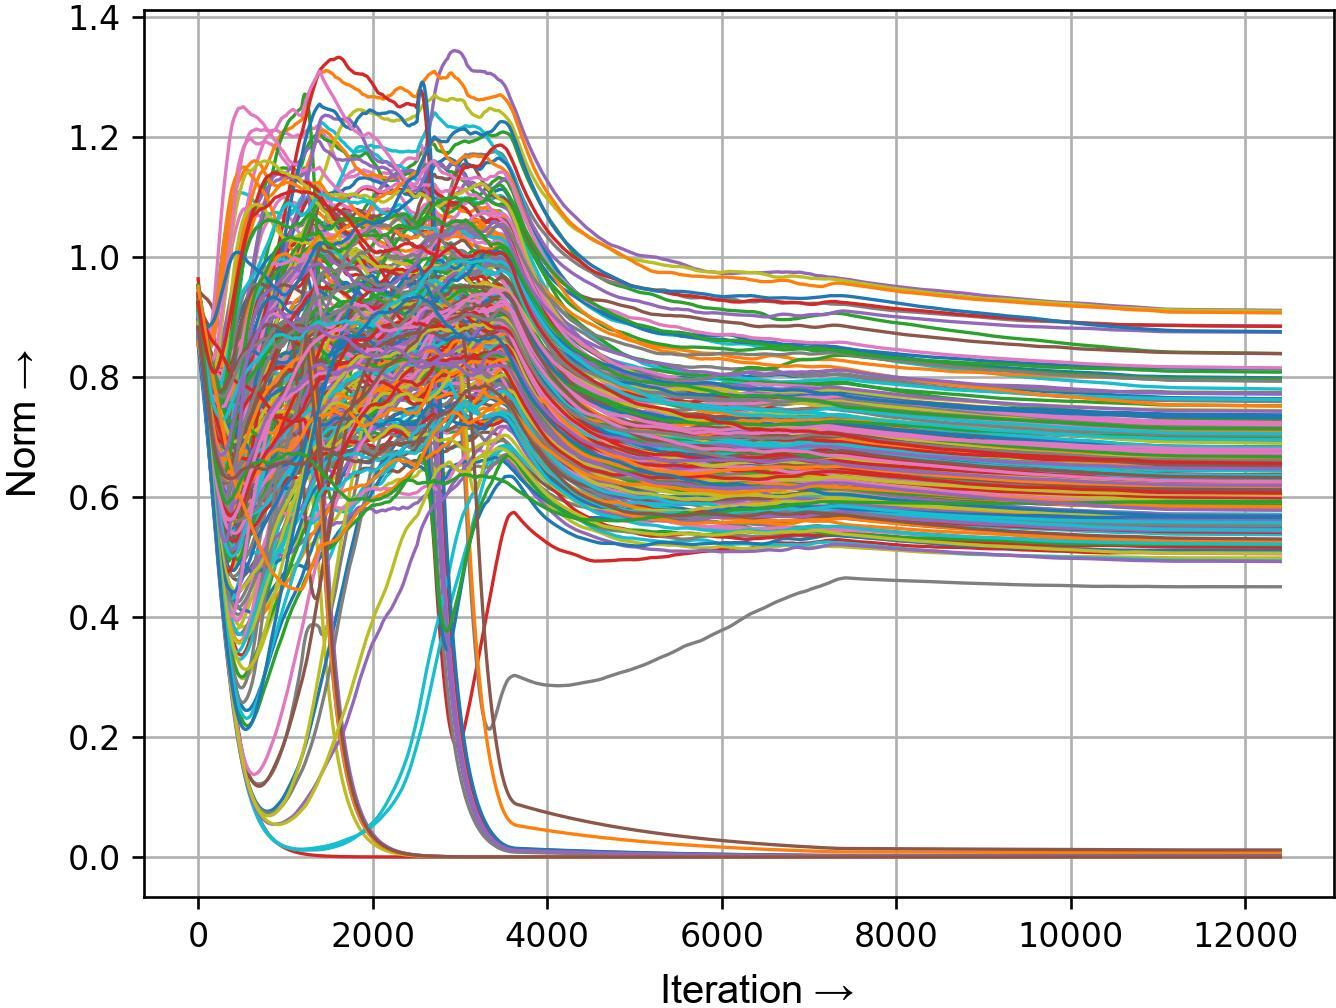
\includegraphics[width=\textwidth]{trimmed/baseline-w-layer-4-2}
\caption{Layer 11\\ \forceindentb\textbf{baseline}}
\end{subfigure}
\begin{subfigure}[t]{0.16\textwidth}
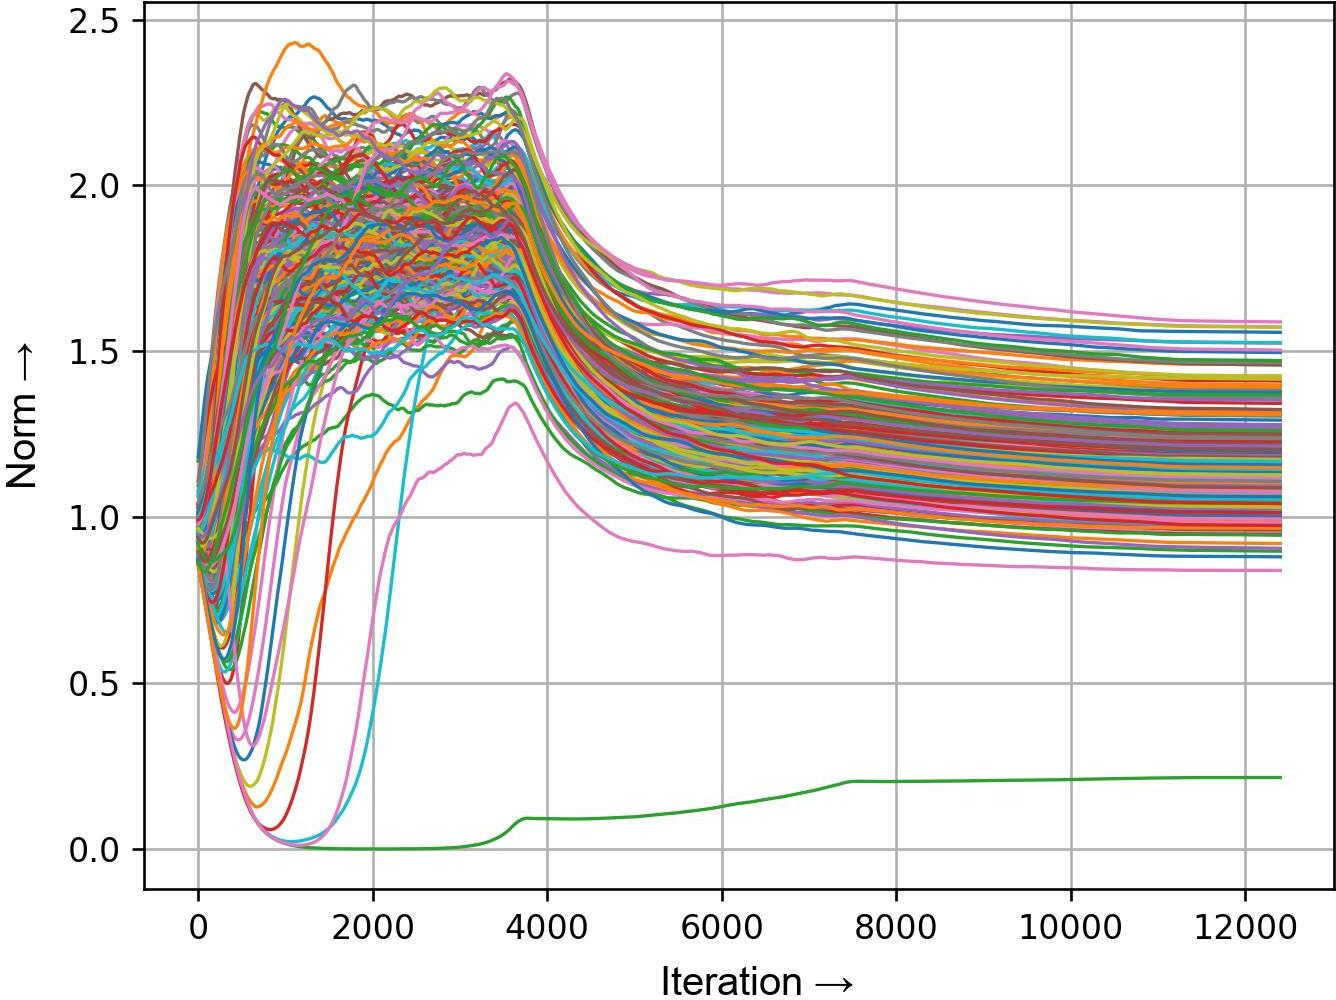
\includegraphics[width=\textwidth]{trimmed/pgt-w-layer-4-2}
\caption{Layer 11\\ \forceindentb\textbf{PGT}}
\end{subfigure}
\begin{subfigure}[t]{0.16\textwidth}
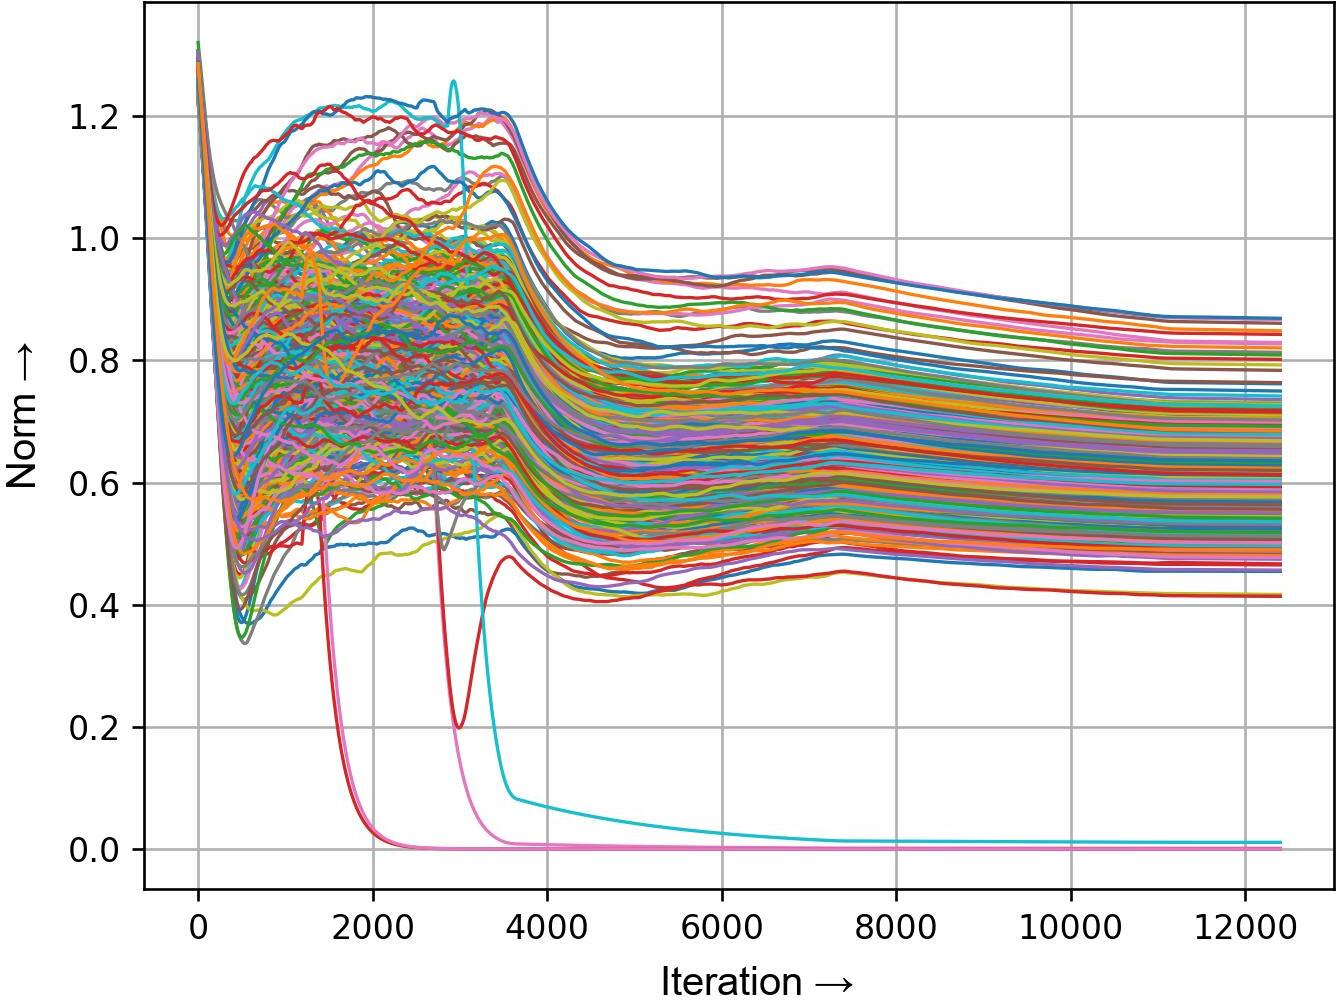
\includegraphics[width=\textwidth]{trimmed/baseline-w-layer-7-2}
\caption{Layer 19\\ \forceindentb\textbf{baseline}}
\end{subfigure}
\begin{subfigure}[t]{0.16\textwidth}
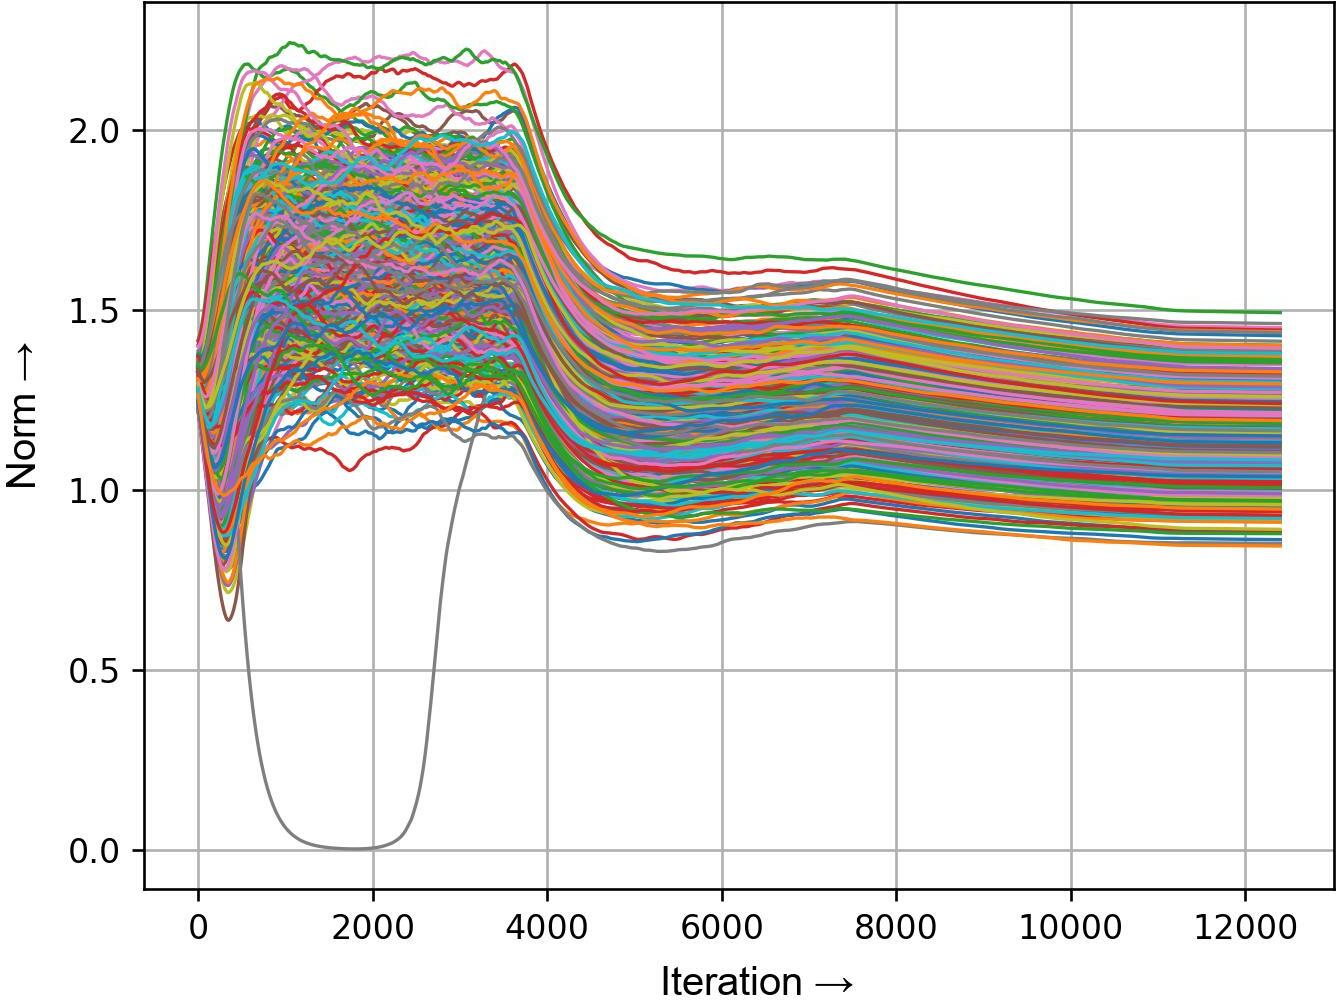
\includegraphics[width=\textwidth]{trimmed/pgt-w-layer-7-2}
\caption{Layer 19\\ \forceindentb\textbf{PGT}}
\end{subfigure}
\begin{subfigure}[t]{0.16\textwidth}
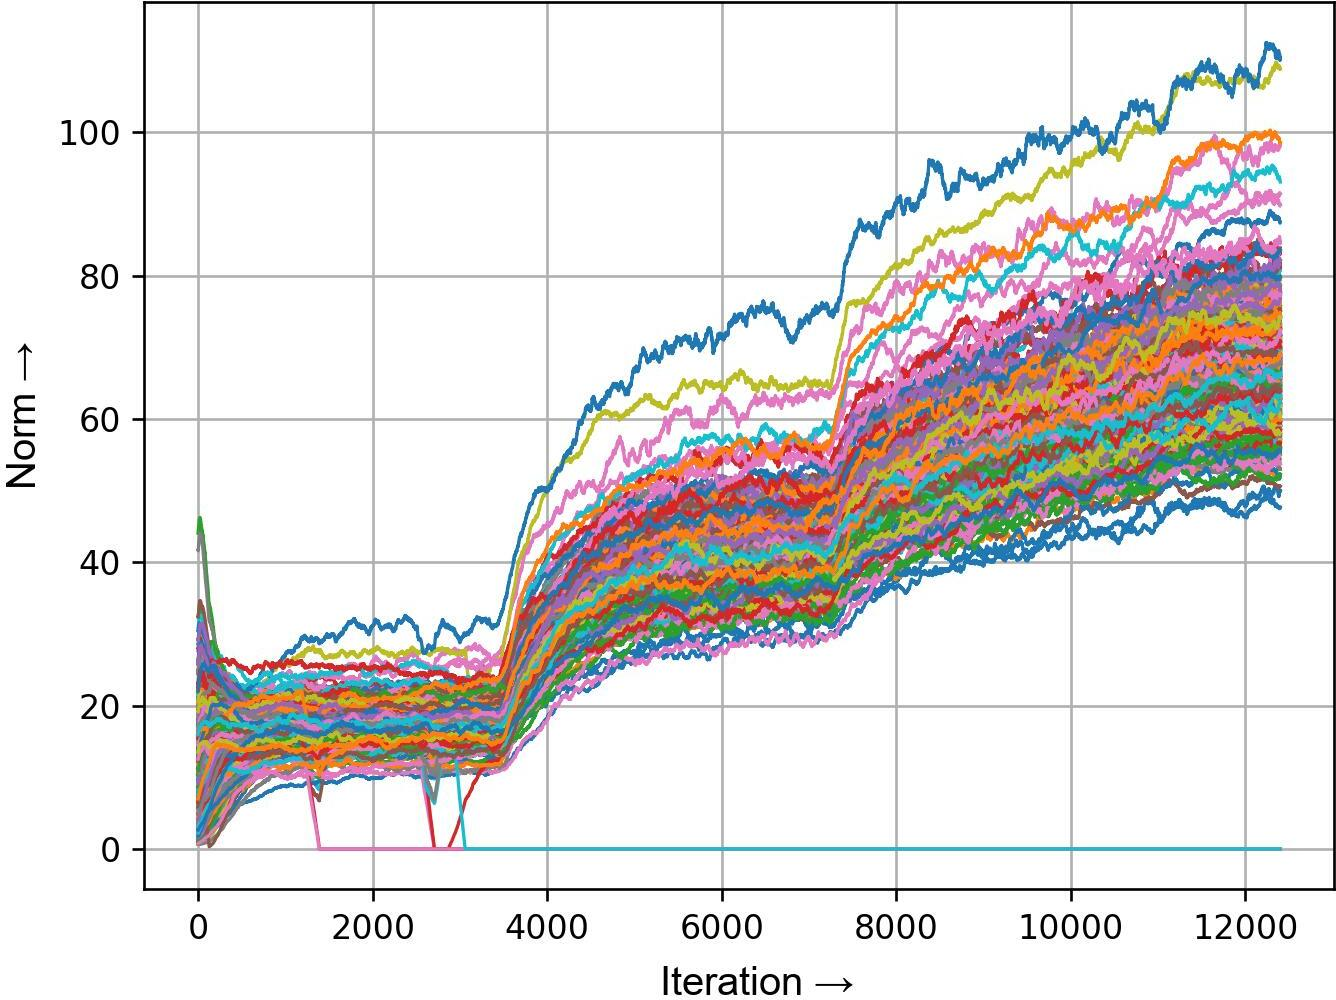
\includegraphics[width=\textwidth]{trimmed/baseline-f-layer-22-1}
\caption{\scriptsize{GAP\\\forceindentb features}\\ \forceindentb\textbf{baseline}}
\end{subfigure}
\begin{subfigure}[t]{0.16\textwidth}
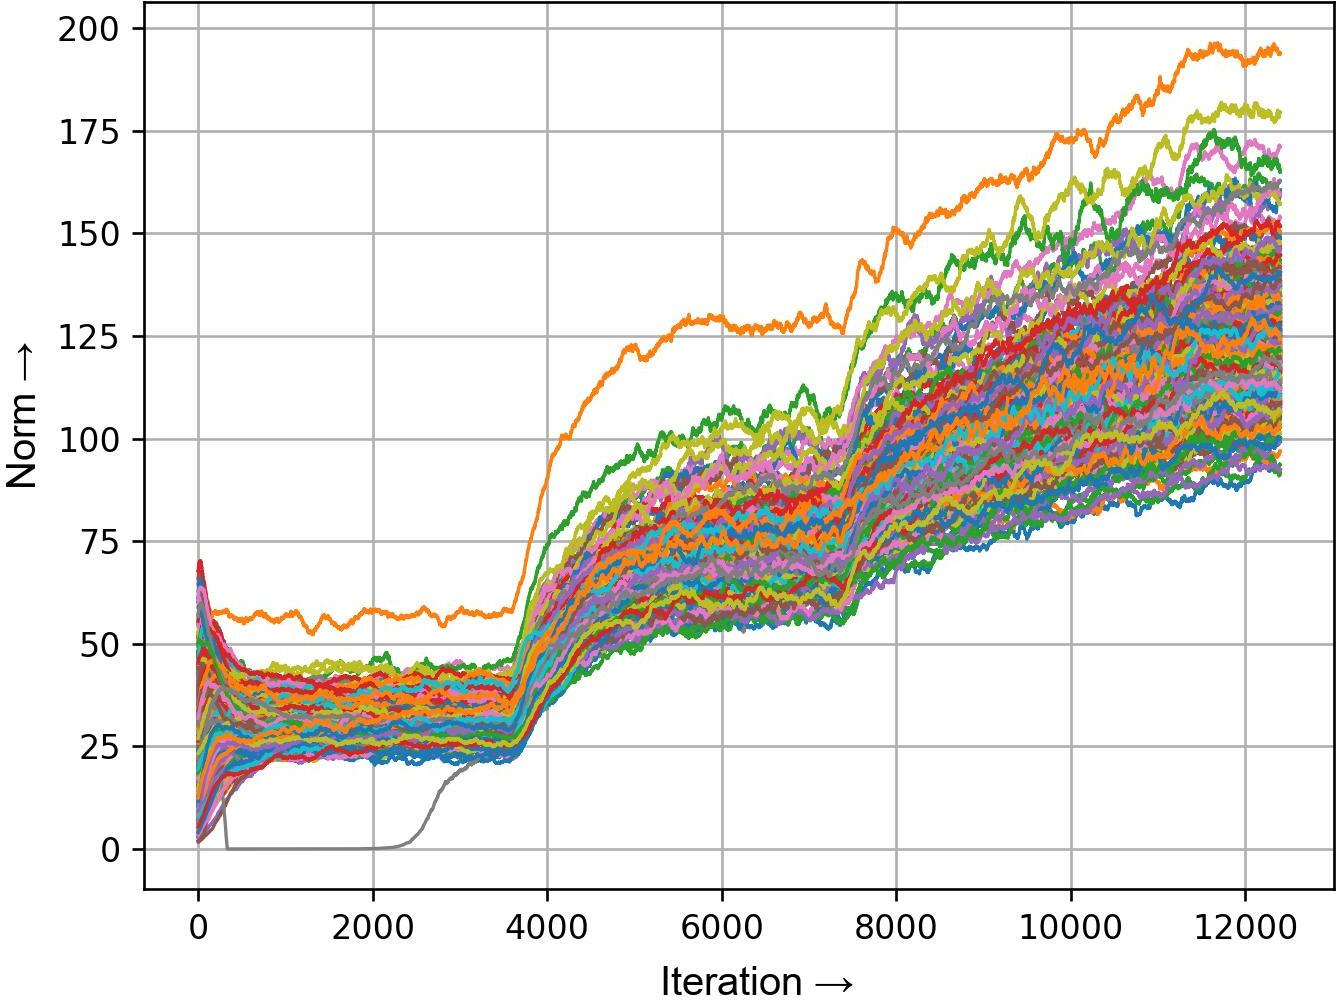
\includegraphics[width=\textwidth]{trimmed/pgt-f-layer-22-1}
\caption{\scriptsize{GAP\\\forceindentb features}\\ \forceindentb\textbf{PGT}}
\end{subfigure}

\vspace{6pt}

\begin{subfigure}[t]{0.16\textwidth}
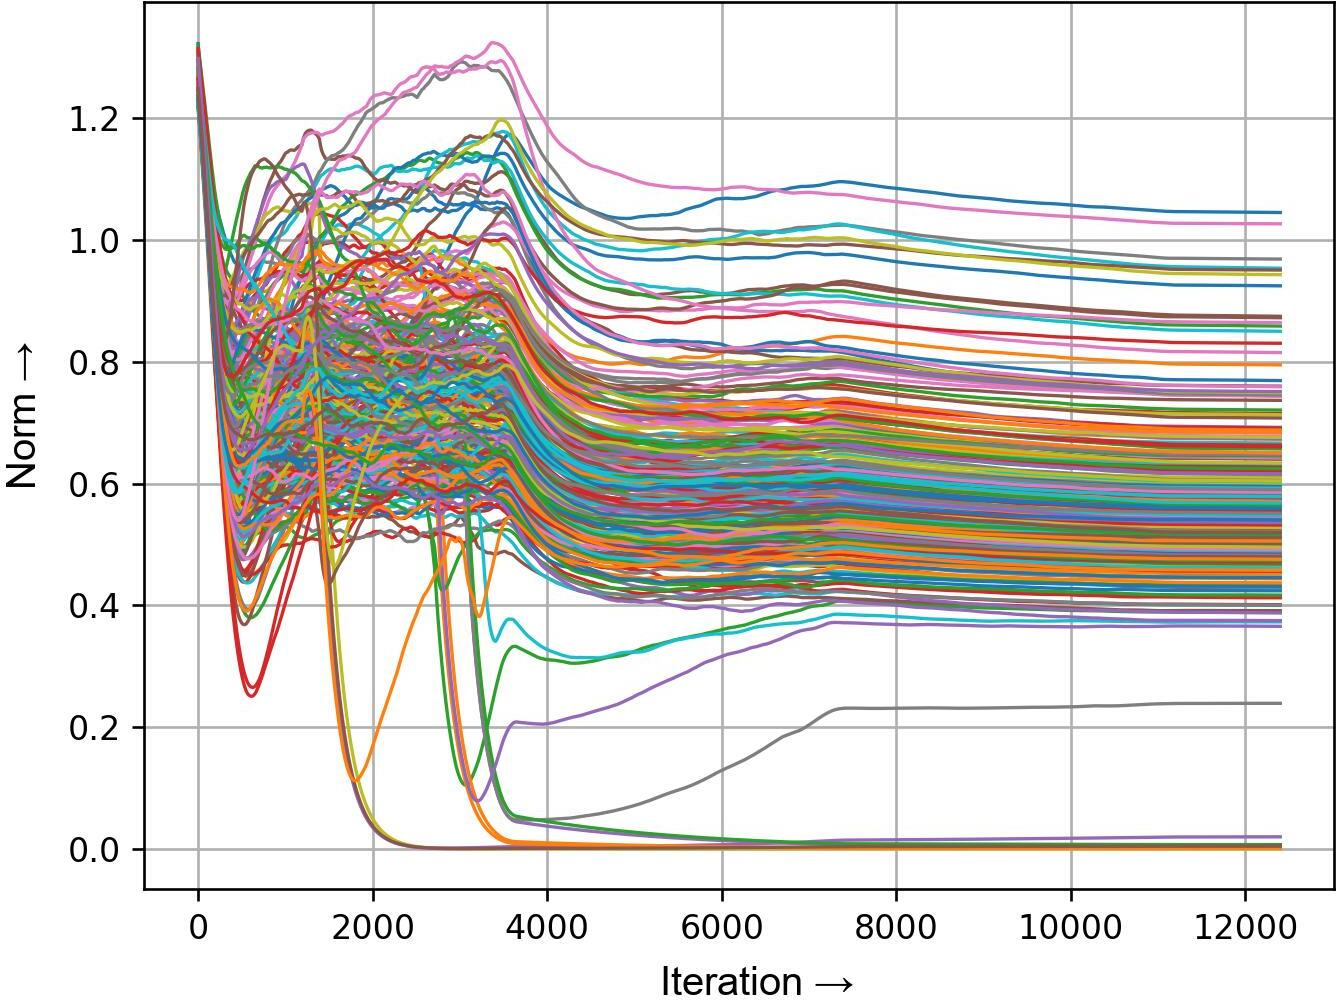
\includegraphics[width=\textwidth]{trimmed/baseline-w-layer-5-3}
\caption{Layer 15\\ \forceindentb\textbf{baseline}}
\end{subfigure}
\begin{subfigure}[t]{0.16\textwidth}
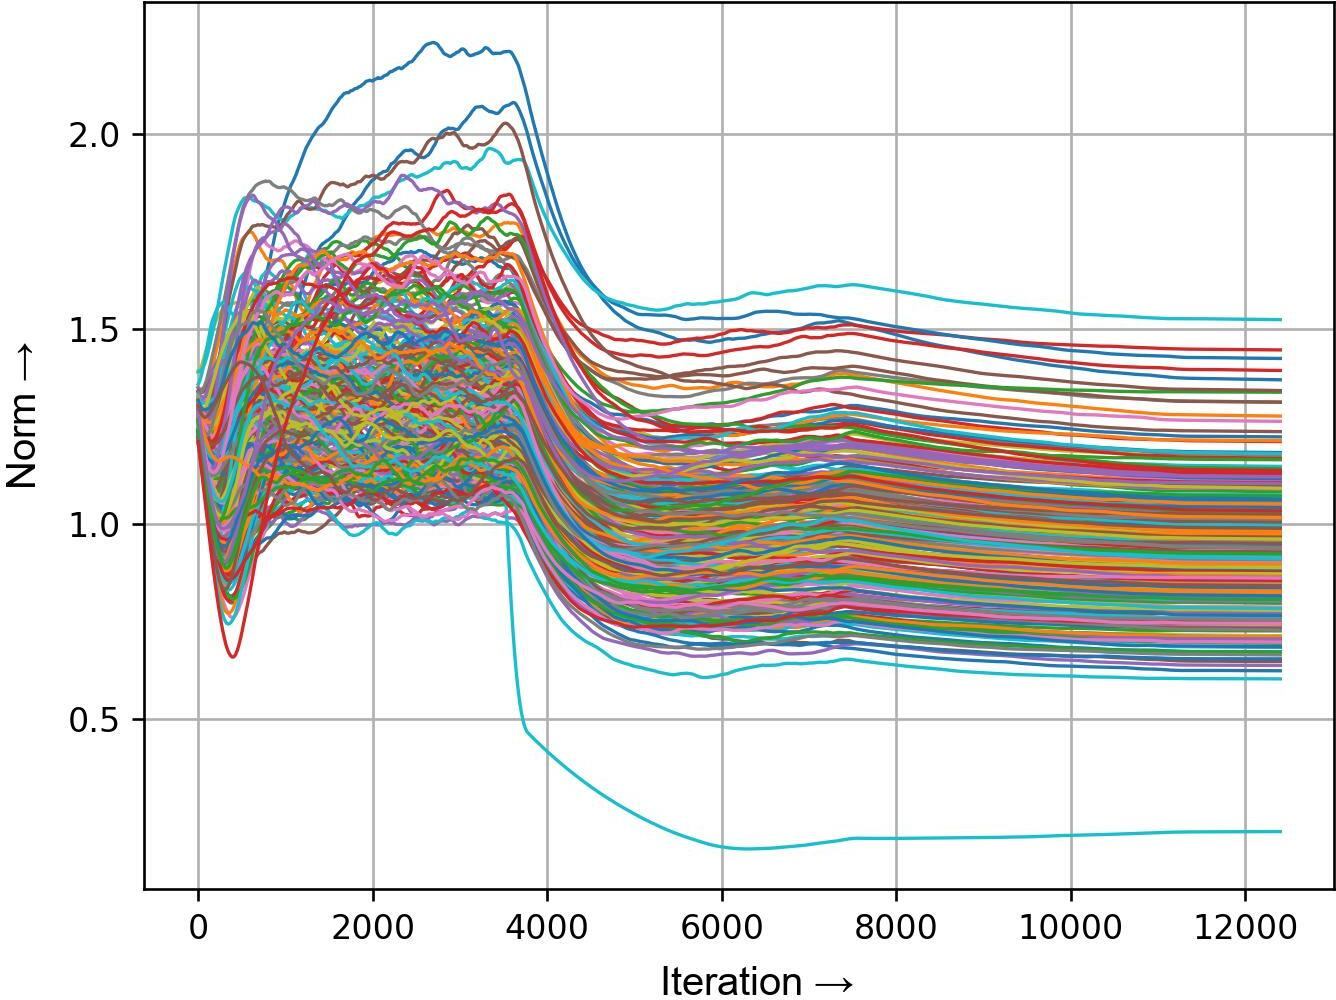
\includegraphics[width=\textwidth]{trimmed/pgt-w-layer-5-3}
\caption{Layer 15\\ \forceindentb\textbf{PGT}}
\end{subfigure}
\begin{subfigure}[t]{0.16\textwidth}
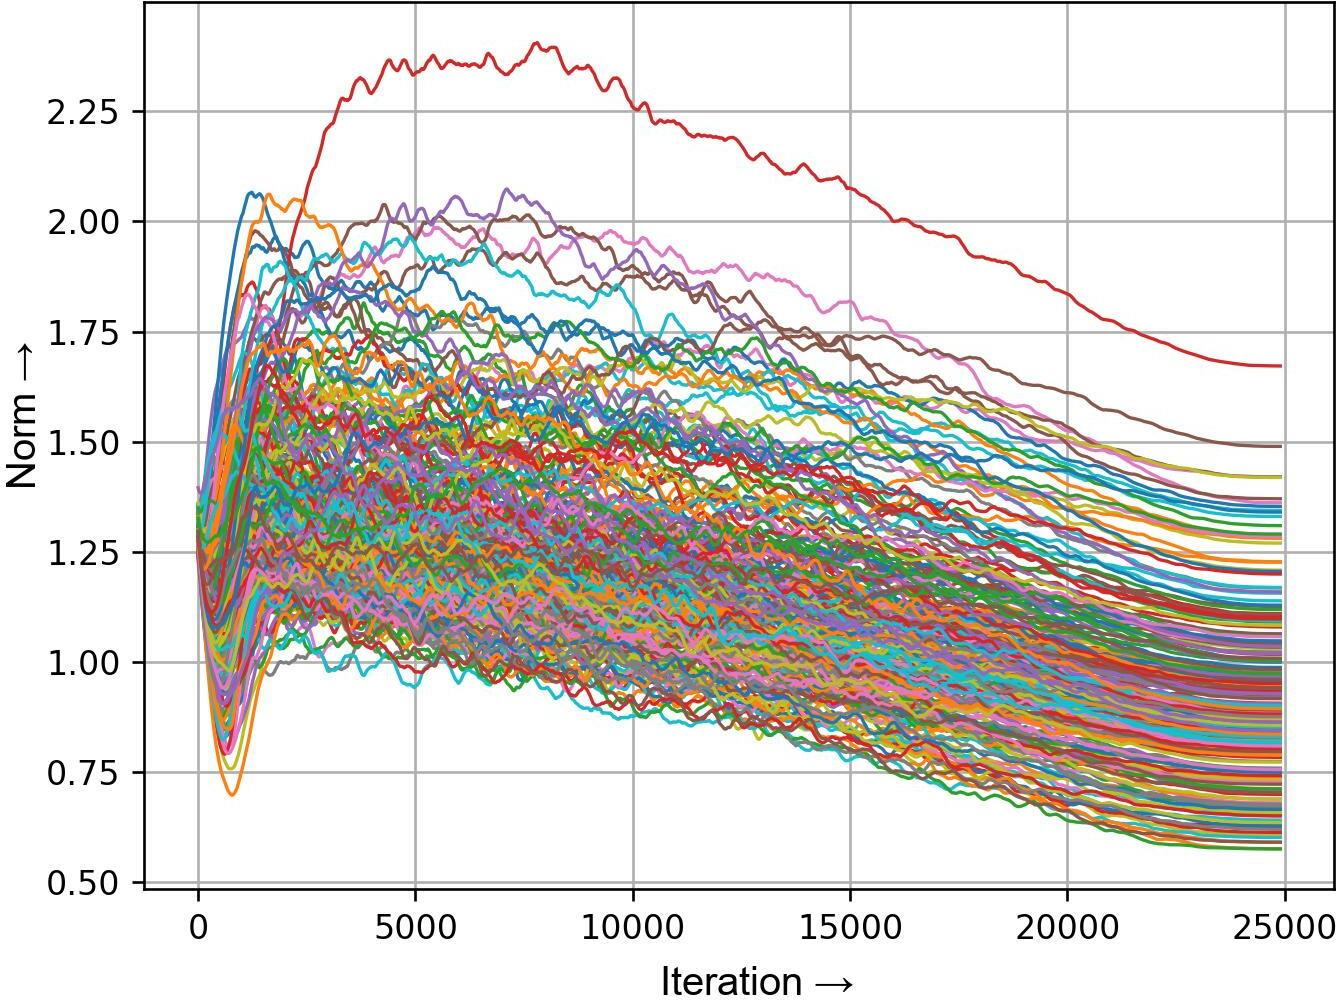
\includegraphics[width=\textwidth]{trimmed/agc_pgt-w-layer-5-3}
\caption{Layer 15\\ \forceindenta\textbf{AGC+PGT}}
\end{subfigure}
\begin{subfigure}[t]{0.16\textwidth}
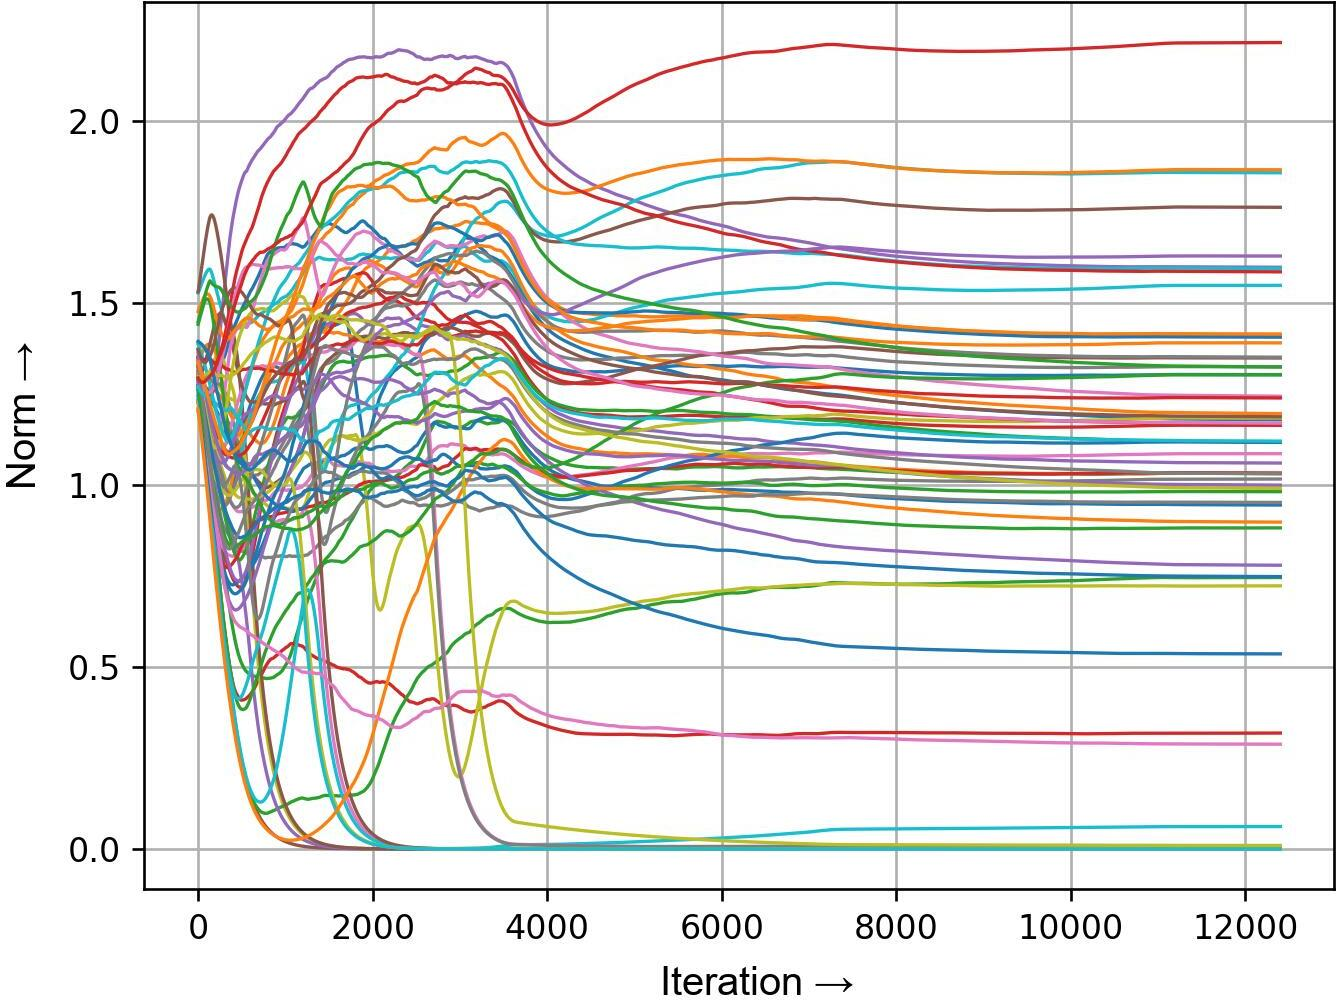
\includegraphics[width=\textwidth]{trimmed/baseline-w-layer-1-2}
\caption{Layer 2\\ \forceindentb\textbf{baseline}}
\end{subfigure}
\begin{subfigure}[t]{0.16\textwidth}
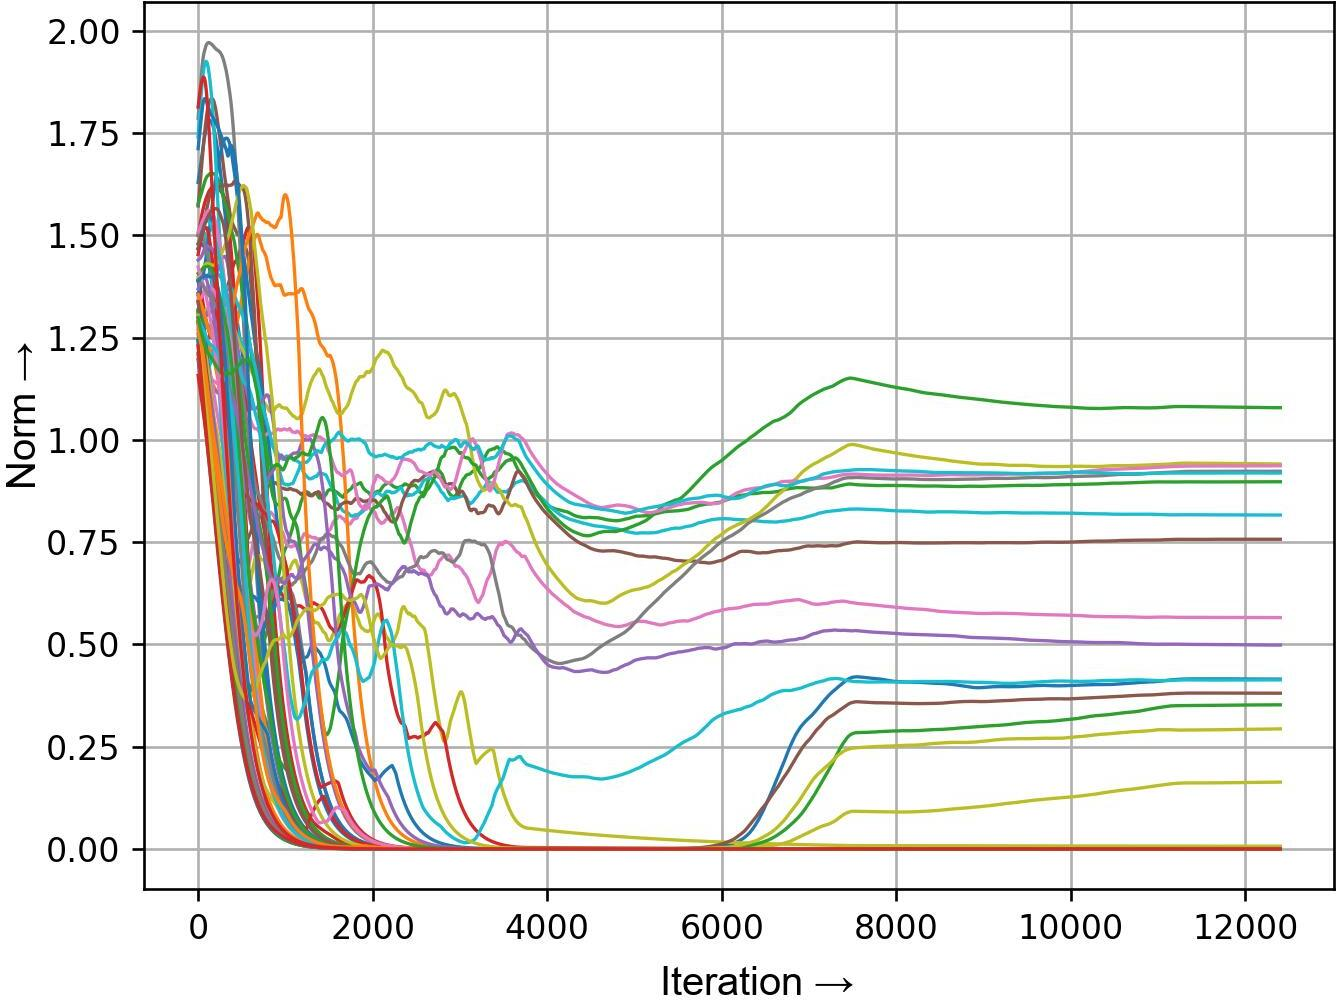
\includegraphics[width=\textwidth]{trimmed/pgt-w-layer-1-2}
\caption{Layer 2\\ \forceindentb\textbf{PGT}}
\end{subfigure}
\begin{subfigure}[t]{0.16\textwidth}
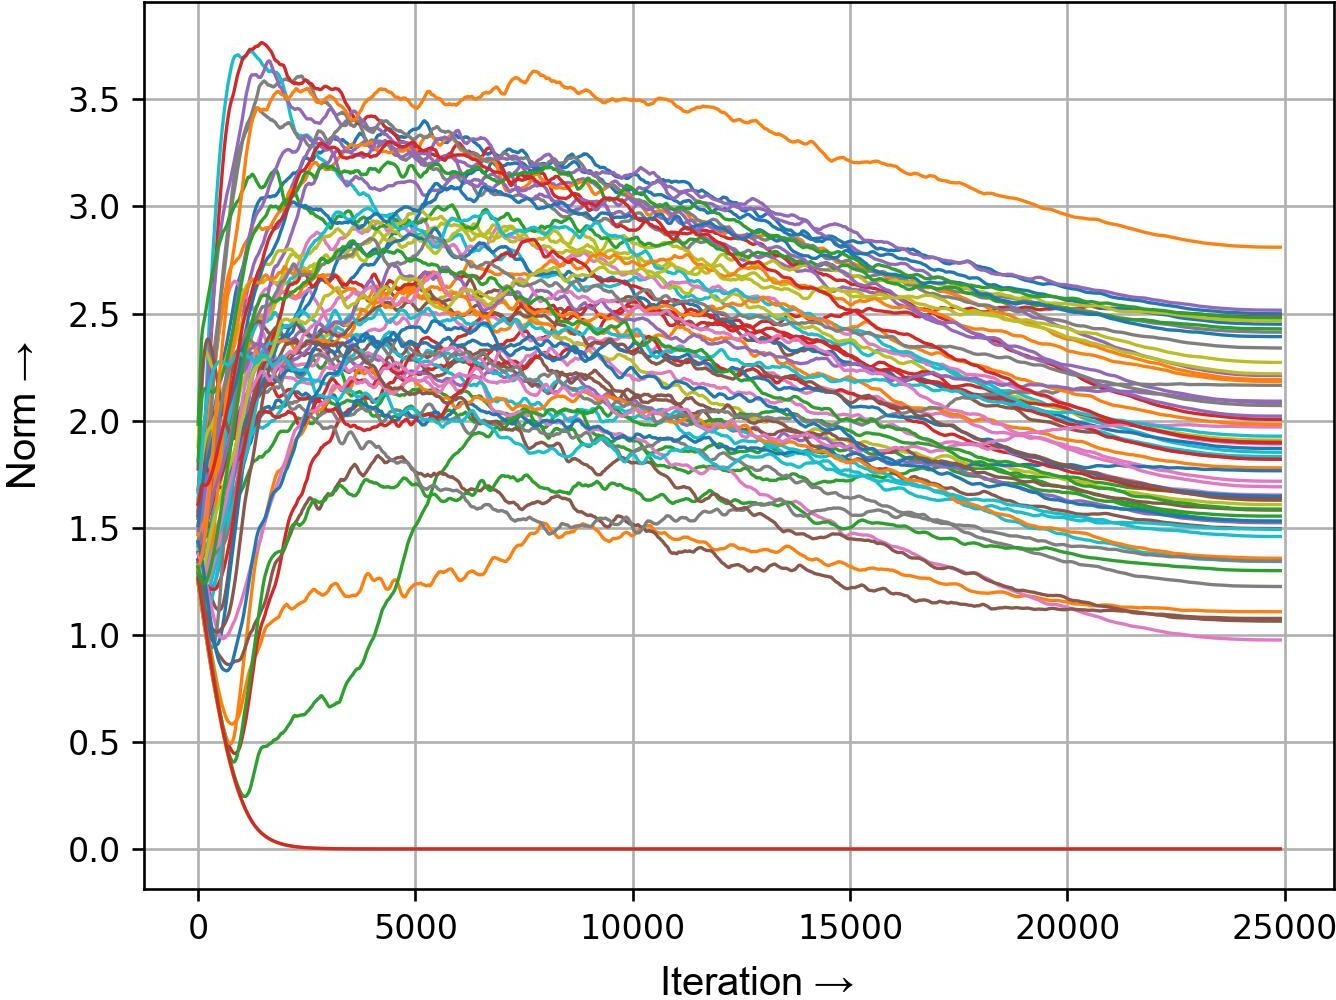
\includegraphics[width=\textwidth]{trimmed/agc_pgt-w-layer-1-2}
\caption{Layer 2\\ \forceindenta\textbf{AGC+PGT}}
\end{subfigure}
\captionsetup{font=normalsize}
\caption{ Norm vs iter. plots demonstrating layer characteristics (the zero out
phenomena) and the efficacy of PGT and AGC+PGT over baseline. Each colour represents a
different filter or feature vector of a particular layer of a non-BN variant of
ResNet-18. Readers are requested to zoom in or refer to section \ref{sec:big_plots} for
a zoomed-in view. }
\label{fig:norm_plots}
\vspace{-0.5cm}
\end{figure}








Fig. \ref{fig:norm_plots}(c) and \ref{fig:norm_plots}(e) are plots of the final conv
layer's filters (layer $19$) and the features output of final global average pooling
(GAP) layer respectively. We observe a number of filters and features in the final layer
completely zeroing out. The feature vector after the GAP layer directly interfaces with
the fully connected layer. Therefore any zeroed out features leads to permanent
information loss, as it does not contribute to the learning of decision boundaries in
the fully connected layer. Also, zeroed out weights tensors lead to zeroed out gradients
hence stopping training for all subsequent iterations leading to a collapse in training
for the affected layers. With large batch sizes, it is possible that an entire layer
zeroes out as shown in the figure below. Gradient modification methods such as PGT or
AGC can alleviate the zeroing out phenomena as we observe that the number of zeroed out
filters has considerably reduced [Fig. \ref{fig:norm_plots}(b, d)]. The final feature
tensor [Fig. \ref{fig:norm_plots}(f)] with PGT enabled, does not contain any zeroed out
regions indicating that information loss is mitigated as the features pass on from the
feature extracting layers to the fully connected layer. When PGT and AGC are combined,
we get the most benefit as we demonstrate for layers $15$ and layer $2$ (Fig
\ref{fig:norm_plots}(g-i)] and Fig \ref{fig:norm_plots}(j-l) respectively).





\begin{table}[!t]
\centering
\caption{ Results for non-normalized ResNets on ImageNet-1K. Best training and test
accuracies are highlighted in red and blue respectively. Top differences in training and
test accuracies are marked in yellow. }
\label{tab:wobn_table}
\begin{tabular}{cccccccc}
\multirow{2}{*}{\textbf{Model}} & \multirow{2}{*}{\textbf{Batch Size}} &
\multirow{2}{*}{\textbf{Method}} & \textbf{PGT} & \textbf{Train}
& \textbf{Train} & \textbf{Test} & \textbf{Test} \\
& & & \textbf{($\alpha$)} & \textbf{Acc.(\%)} & \textbf{Diff(\%)} &
\textbf{Acc.(\%)} & \textbf{Diff(\%)} \\
\midrule
ResNet-18 & 1024 & Baseline & - & 66.27 & - & 64.816 & - \\
(non-BN) & 1024 & PGT & 0.92 & \textcolor{red}{\textbf{66.62}} &
\textcolor{olive}{\textbf{+0.35}} & \textcolor{blue}{\textbf{65.498}} &
\textcolor{olive}{\textbf{+0.682}} \\
\cmidrule{2-8}
& 512 & Baseline & - & 68.02 & - & 66.552 & - \\
& 512 & PGT & 0.25 & \textcolor{red}{\textbf{69.5}} & \textcolor{olive}{\textbf{+1.48}}
& \textcolor{blue}{\textbf{67.236}} & \textcolor{olive}{\textbf{+0.684}} \\
\cmidrule{2-8}
& 256 & Baseline & - & 68.86 & - & 66.796 & - \\
& 256 & GC & - & 69.04 & +0.18 & 67.064 & +0.268 \\
& 256 & AGC & - & 69.06 & +0.2 & 67.298 & +0.502 \\
& 256 & PGT & 0.25 & \textcolor{red}{\textbf{69.97}} & \textcolor{olive}{\textbf{+1.11}}
& \textcolor{blue}{\textbf{67.814}} & \textcolor{olive}{\textbf{+1.018}} \\
\cmidrule{2-8}
& 256 & Baseline & - & 68.86 & - & 66.796 & - \\
& 256 & GC+PGT & 0.25 & 68.67 & -0.19 & 67.088 & +0.292 \\
& 256 & AGC+PGT & 0.25 & \textcolor{red}{\textbf{70.92}} &
\textcolor{olive}{\textbf{+2.06}} & \textcolor{blue}{\textbf{68.856}} &
\textcolor{olive}{\textbf{+2.06}} \\
\end{tabular}
\vspace{-0.5cm}
\end{table}




In Table \ref{tab:wobn_table} we find that the baseline performance for high batch sizes
($1024$) is drastically inferior to baselines for other batch sizes. PGT helps regain
some of the lost performance by $0.682\%$ ($65.498\%$ vs. $64.816\%$). At a batch size
of 512, invoking PGT improves the training accuracy baseline by $1.48\%$ and the test
accuracy baseline by $0.684\%$, while at a batch size of 256, the improvement in
training and test accuracies are $1.11\%$ and $1.018\%$ respectively. In comparison, the
test accuracy improvements obtained by GC and AGC at batch size of 256


\begin{wrapfigure}{l}{0.4\textwidth}
\vspace{-1cm}
\centering
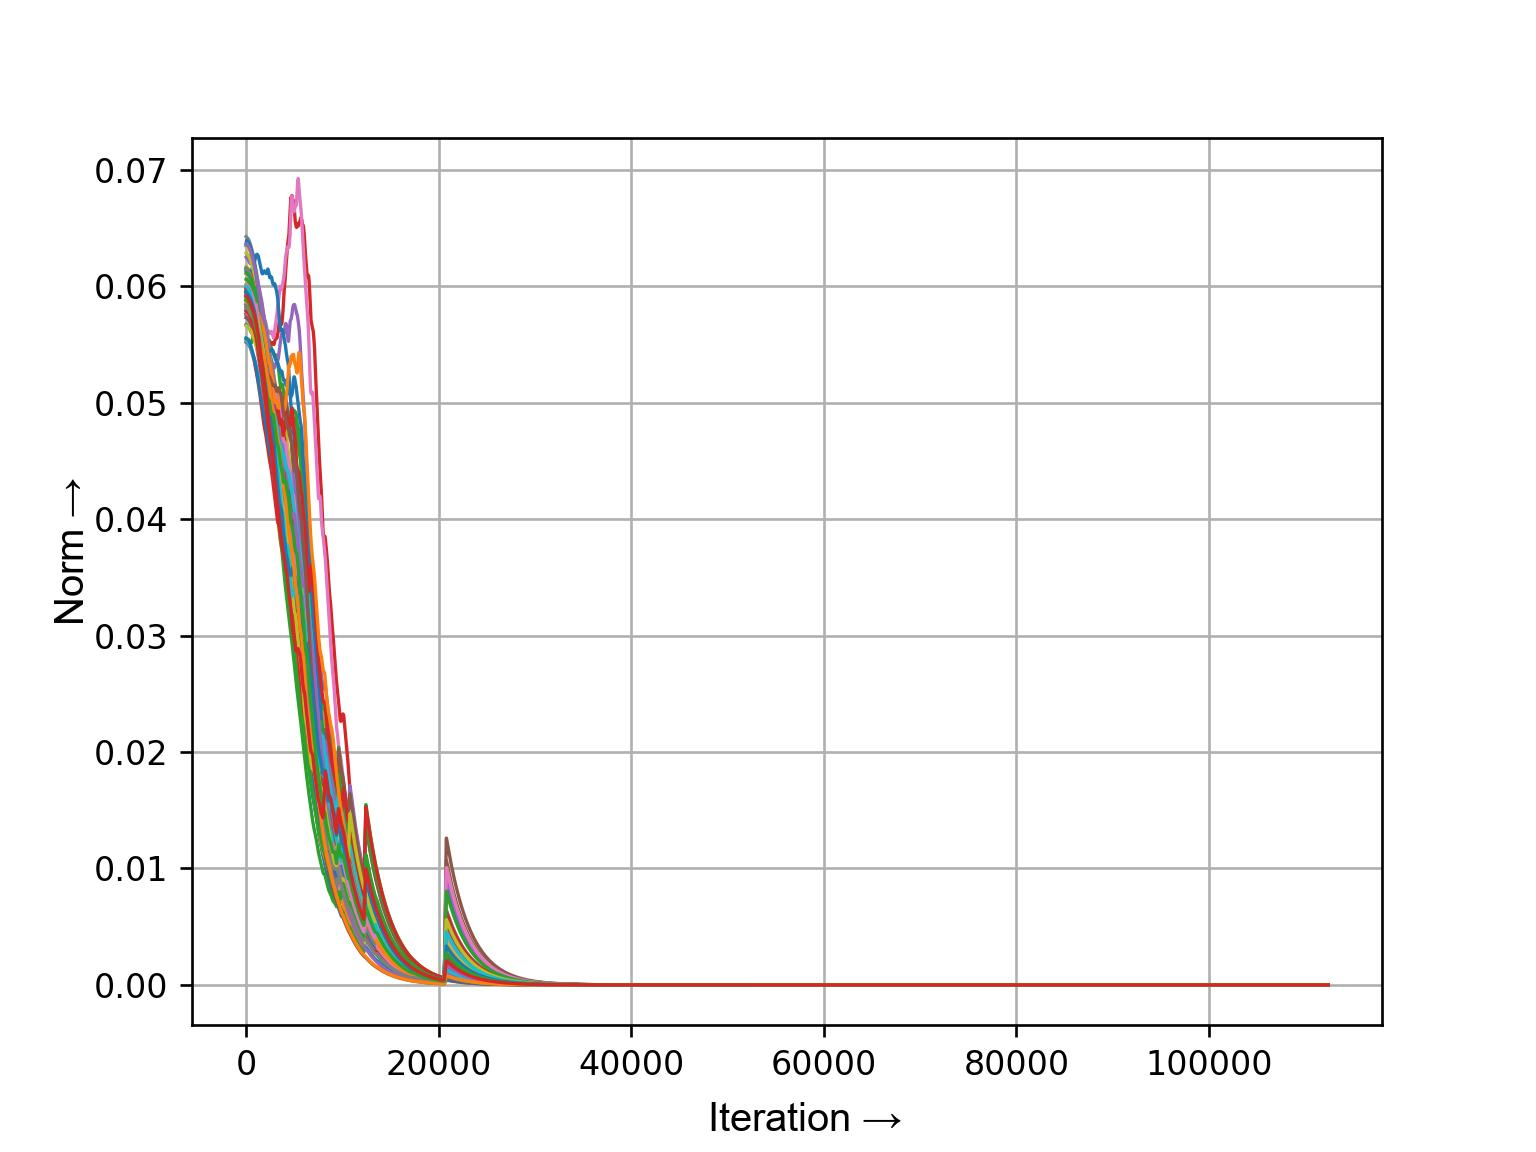
\includegraphics[width=0.45\textwidth]{baseline_high_bs-w-layer2-2}
\vspace{-1.5cm}
\end{wrapfigure}

\noindent
is much less at $0.27\%$ and $0.5\%$, respectively. On the training accuracy front,
since we get a significant boost ($1.48\%$ at batch size of 512 and $1.11\%$ at batch
size of 256), it leads us to infer that when PowerGrad Transform is used, the network
fits the training dataset more tightly and the convergence optima is significantly
superior. Combining GC with PGT is not very significant. When AGC and PGT are combined,
we see a tremendous increase in test accuracy of over $2.06\%$ over the baseline.
Additionally, we provide comprehensive graphs of the norm profiles of the AGC + PGT
method for all layers in the supplementary section \ref{sec:plots1}\ -\
\ref{sec:plots4}.










\subsection{Effect on Loss, Logits and other metrics}
\label{sec:Effe}



\begin{figure}[!t]
\centering
\begin{subfigure}{0.33\textwidth}
\centering
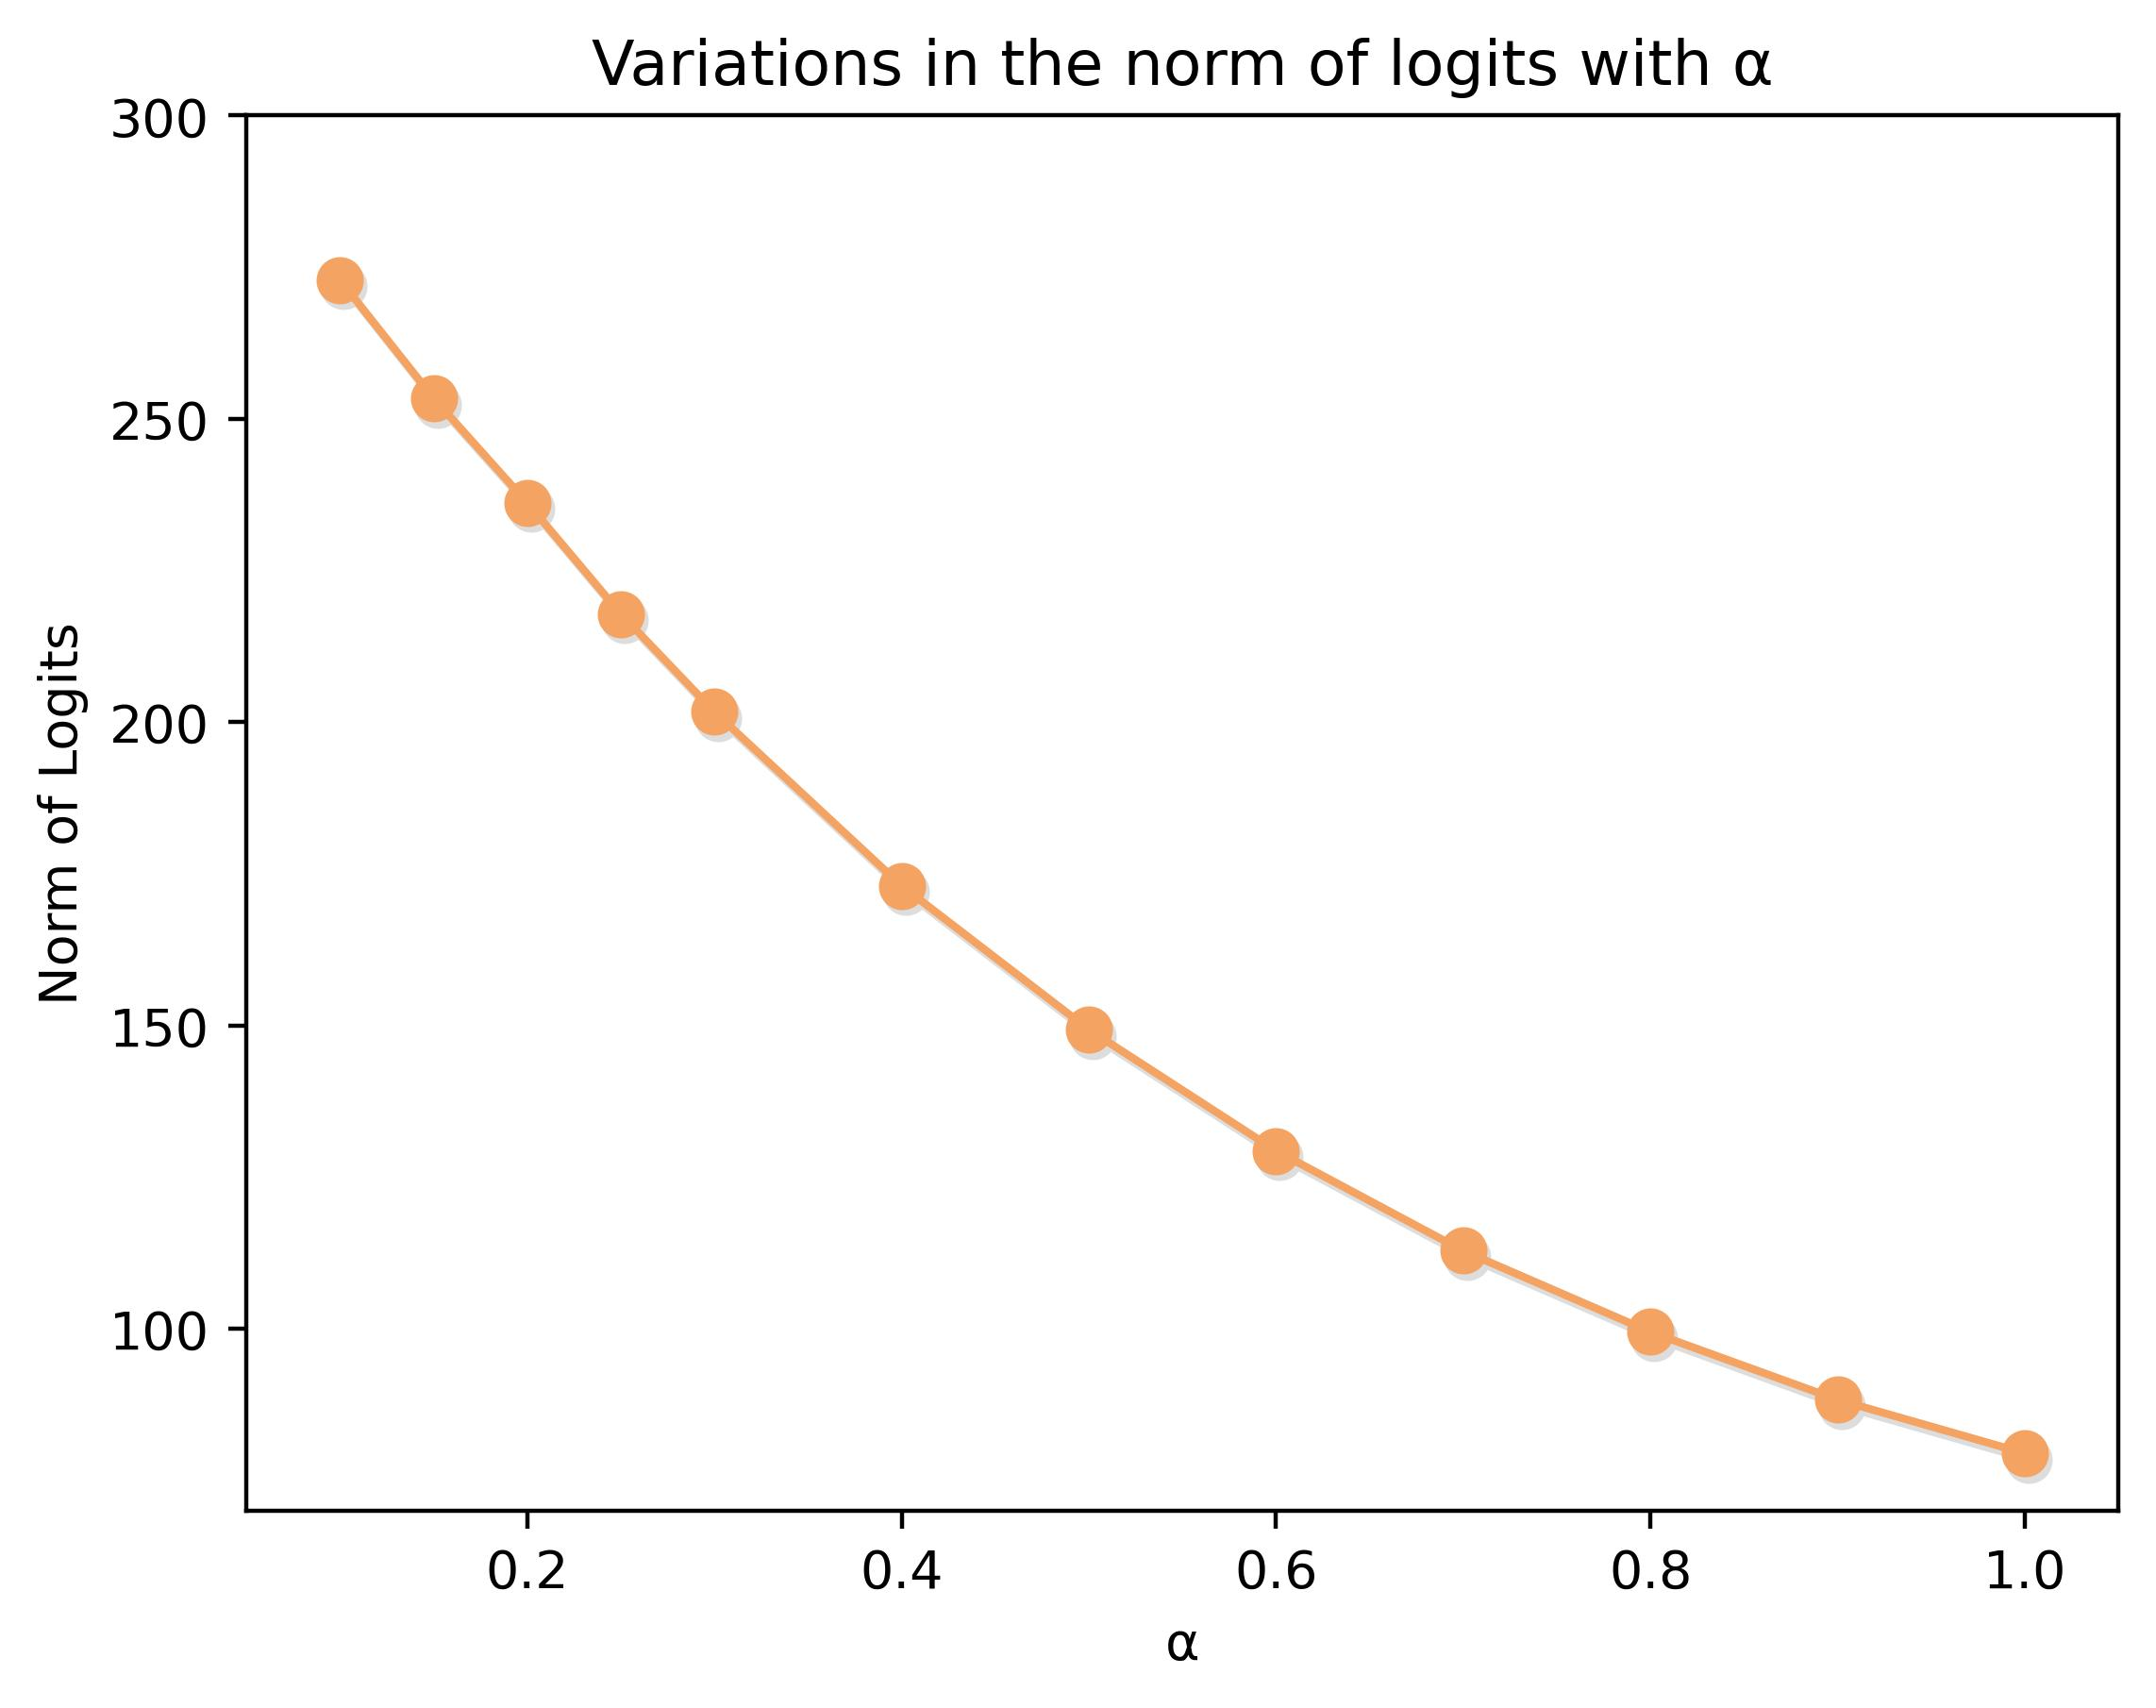
\includegraphics[width=0.98\textwidth]{logit_vs_alpha}
\caption{\\Logit vs. $\alpha$}
\end{subfigure}%
\begin{subfigure}{0.33\textwidth}
\centering
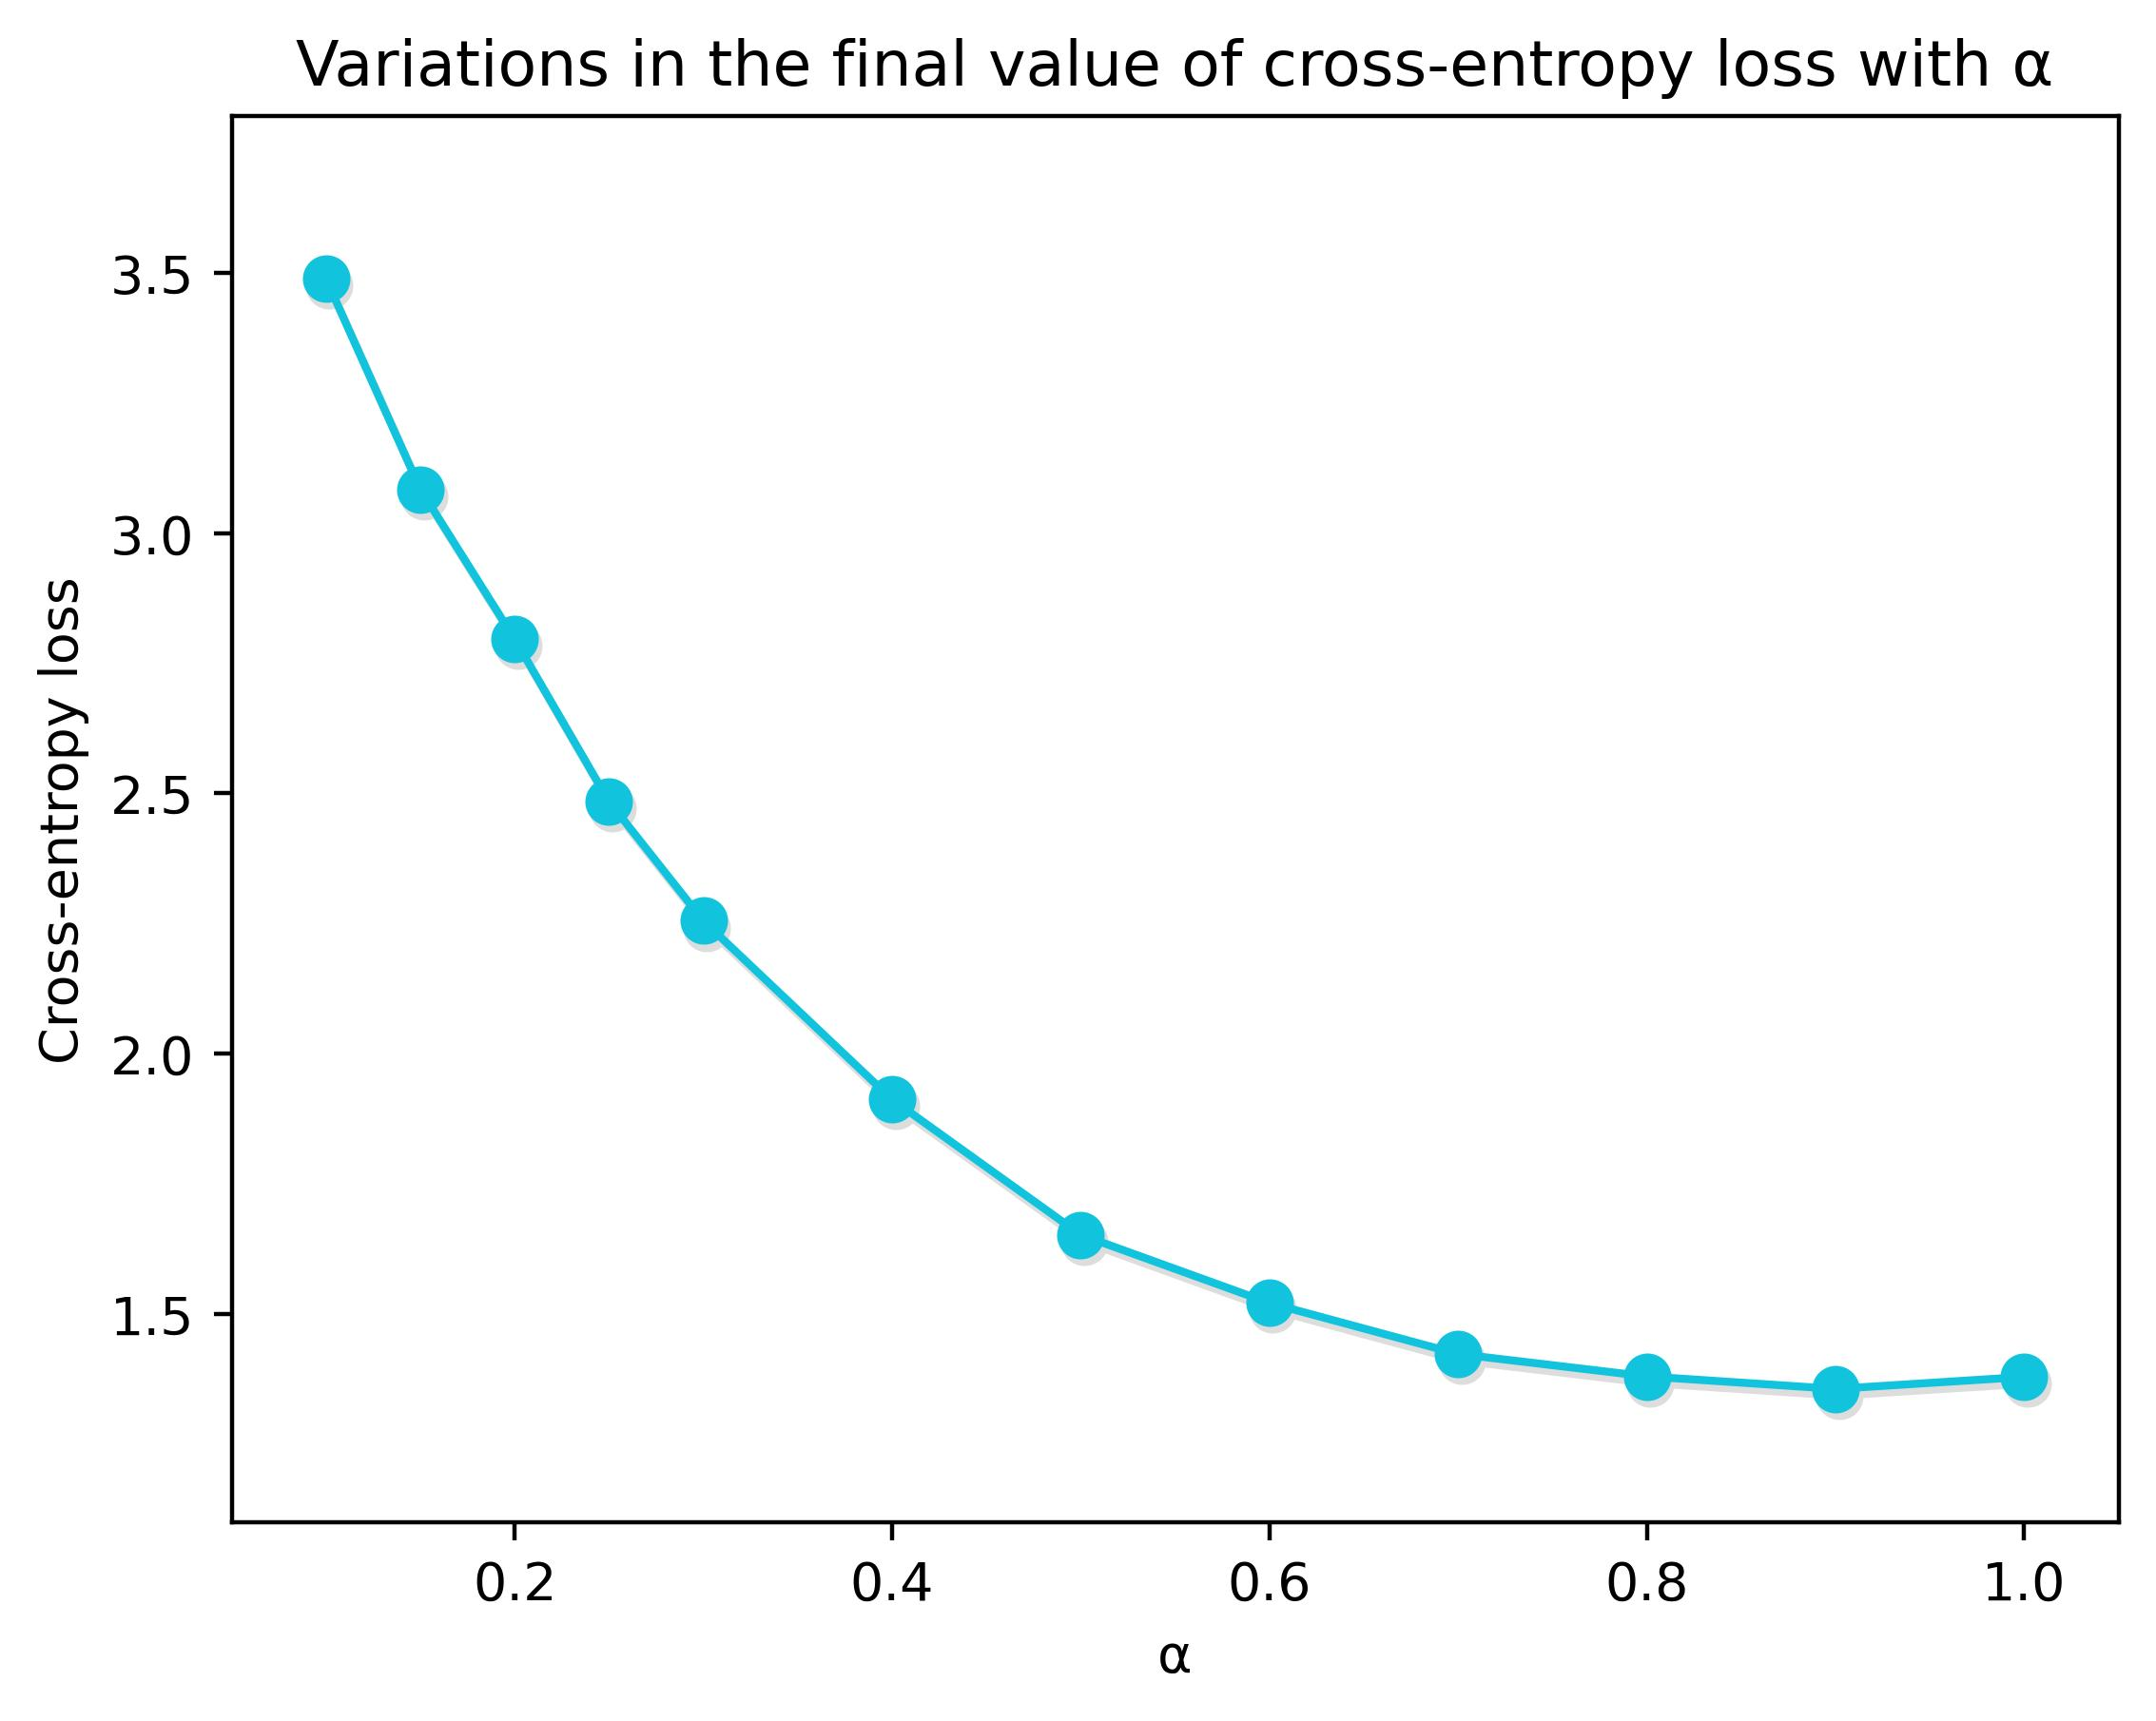
\includegraphics[width=0.98\textwidth]{loss_vs_alpha}
\caption{\\Cross-entropy loss vs. $\alpha$}
\end{subfigure}%
\begin{subfigure}{0.33\textwidth}
\centering
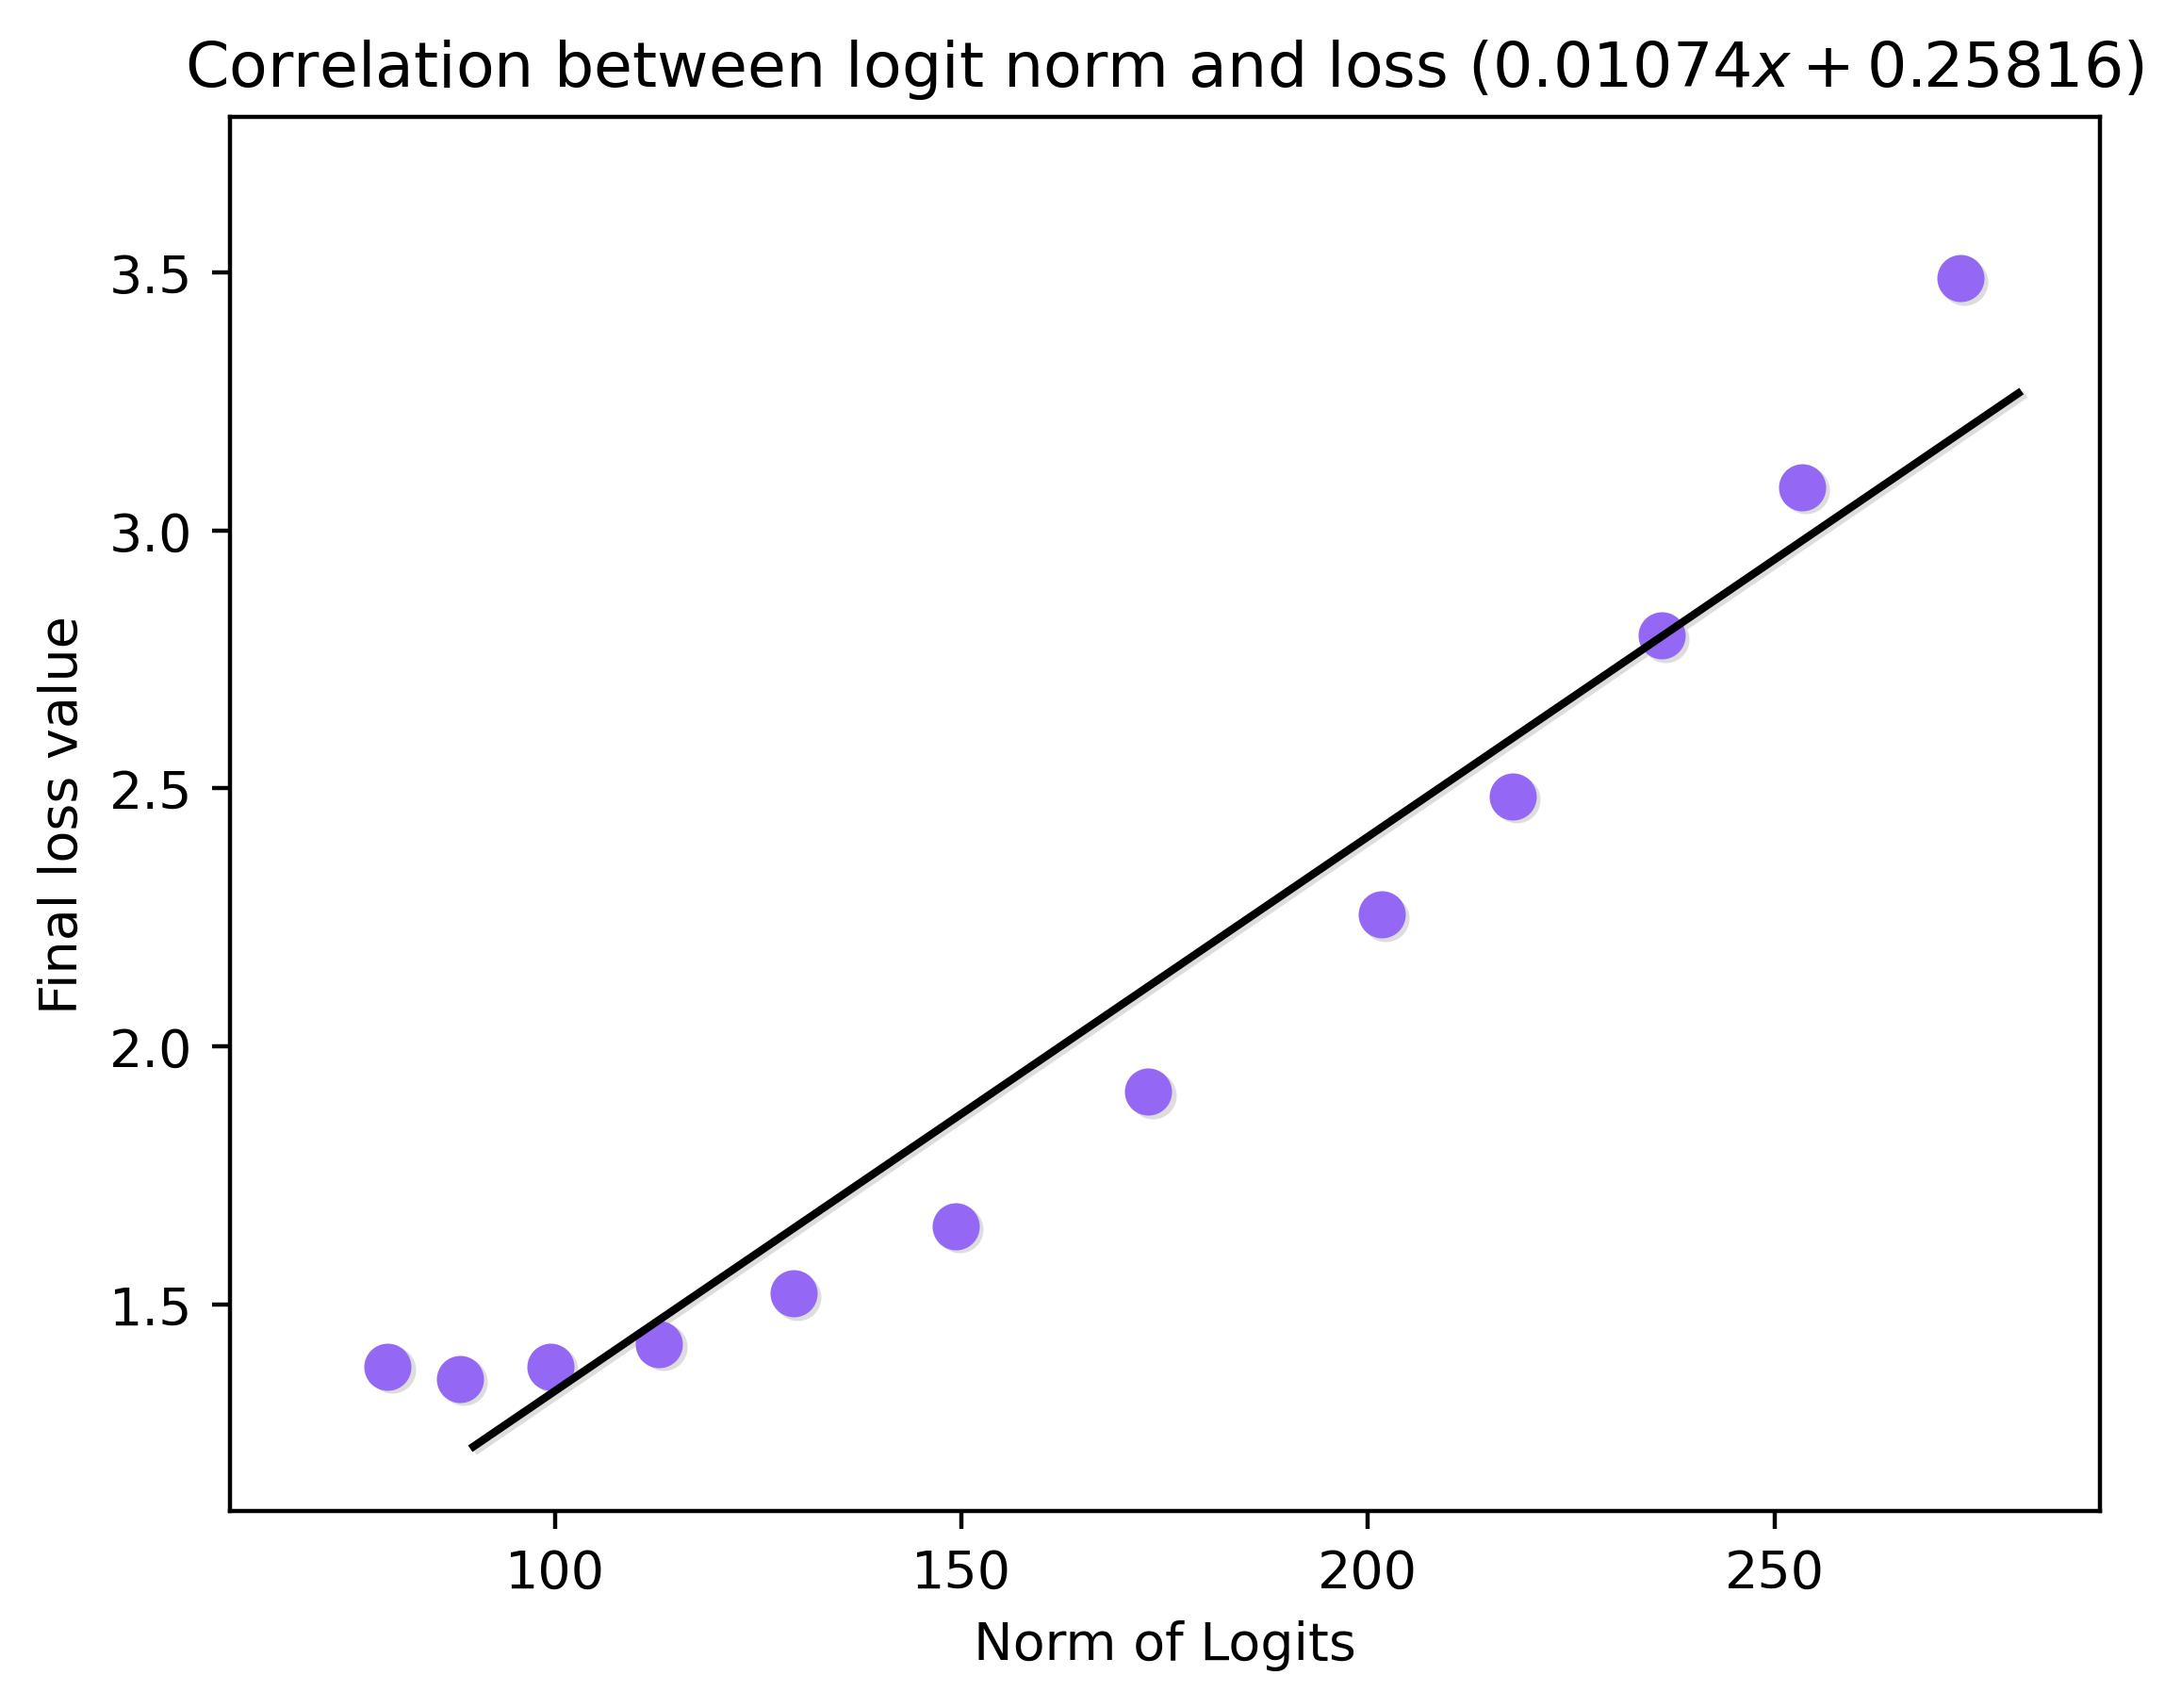
\includegraphics[width=0.98\textwidth]{logit_vs_loss}
\caption{\\Logit-Loss correlation}
\end{subfigure}
\caption{ Plots of various statistical measures: \textbf{(a)} Variations in the logit
norm vs. $\alpha$. The logit norm is calculated per image over the test set of
ImageNet-1K (at the linear layer of the ResNet-18 architecture) and then averaged.
\textbf{(b)} Variations in the final loss values obtained for different $\alpha$
settings. \textbf{(c)} Correlation between loss and logits. Regression line equation:
$(0.01074 x + 0.25816)$. }
\label{fig:stats}
\vspace{-0.5cm}
\end{figure}





As seen in Fig. \ref{fig:stats}(a), the logit norm increases as $\alpha$ falls from $1$
to $0$. We also see that the final value of the loss rises as $\alpha$ drops, and that
the logit norm and the final value of the loss are linearly correlated Fig.
\ref{fig:stats}(c). What is surprising is that: \textit{it is possible to achieve higher
accuracies even though the loss values are larger during convergence}. In our studies
with ResNet-50, for instance, if PGT is not invoked, the corresponding test accuracy is
$76.56\%$ [Table \ref{tab:imagenet_table}] with a cross-entropy loss value of $0.852$.
However, if PGT is activated with $\alpha=0.05$, the corresponding test accuracy is
$77.216\%$ [Table \ref{tab:imagenet_table}] with a loss value of $2.360$. This is
markedly different from the coupled gradient descent based training procedures. PGT
enables the network to arrive at such optima where the loss values are high, but both
training and test perfomance is better. From these plots of logits and losses we find
that with the inclusion of PGT in the training process, the model can have access to
such regions of the loss landscape that is otherwise inaccessible to traditional
gradient based training procedures.

\section{Ablation Study}
\label{sec:Abla}


\begin{table}[!t]
\centering
\caption{ Ablation study for ResNet-50 on ImageNet-1K. }
\label{tab:ablation_table}
\begin{tabular}{cccccccc}
\multirow{2}{*}{\textbf{\#Row}} & \multirow{2}{*}{\textbf{Model}} &
\multirow{2}{*}{\textbf{Scheduler}} & \textbf{Label} & \textbf{PGT} &
\textbf{Train} & \textbf{Test} & \multirow{2}{*}{\textbf{Gap(\%)}} \\
& & & \textbf{Smoothing} & \textbf{($\alpha$)} & \textbf{Acc.(\%)} &
\textbf{Acc.(\%)} & \\
\midrule
1. & ResNet-50 & Step & \xmark & \xmark & 78.99 & 75.97 & 3.02 \\
2. & ResNet-50 & Step & \xmark & 0.3 & 79.56 & 76.494 & 3.066 \\
\cmidrule{2-8}
3. & ResNet-50 & Cosine & \xmark & \xmark & 79.18 & 76.56 & 2.62 \\
4. & ResNet-50 & Cosine & 0.1 & \xmark & 78.81 & 76.698 & 2.112 \\
\cmidrule{2-8}
5. & ResNet-50 & Cosine & \xmark & 0.3 & 79.43 & 76.886 & 2.544 \\
6. & ResNet-50 & Cosine & 0.1 & 0.3 & 78.47 & 76.968 & 1.502 \\
\cmidrule{2-8}
7. & ResNet-50 & Cosine & \xmark & 0.05 & 79.68 & 77.216 & 2.464 \\
8. & ResNet-50 & Cosine & 0.1 & 0.05 & 77.69 & 76.39 & 1.3 \\
\end{tabular}
\vspace{-0.5cm}
\end{table}




We conduct ablation studies to investigate the effects of PowerGrad Transform for
different values of the hyperparameter ($\alpha$), where we use the ResNet-50
architecture and combine our proposed method with different schedulers, regularization
techniques and different values of $\alpha$. We report our findings in Table
\ref{tab:ablation_table}. First we examine the effect of PGT on the step scheduler
baseline in order to later compare it to the cosine scheduler baseline. \textbf{Row-1)}
We begin with the step scheduler baseline ($75.97\%$). \textbf{Row-2)} PGT improves upon
the step scheduler baseline (test set) by a substantial margin with $0.524\%$
($76.494\%$ as opposed to $75.97\%$). \textbf{Row-3)} Introducing the cosine scheduler
yields a $0.59\%$ improvement ($76.56\%$ vs. $75.97\%$) over the step scheduler.
\textbf{Row-4)} After introducing label smoothing, the test accuracy relative to the
cosine scheduler baseline increases by only $0.138\%$ (from $76.56\%$ to $76.698\%$).
\textbf{Row-5)} However, introducing PGT with $\alpha=0.3$ alone (without label
smoothing) improves the cosine scheduler baseline by $0.326\%$ ($76.886\%$ vs.
$76.56\%$). \textbf{Row-6)} Combining PGT ($\alpha=0.3$) with label smoothing improves
the performance on the test set further by $0.408\%$ (from $76.56\%$ to $76.968\%$) and
reduces the generalization gap (from $2.54\%$ to $1.5\%$). However, the impact of
combining PGT with label smoothing can vary depending on the value of the hyperparameter
($\alpha$). \textbf{Row-7)} With a PGT hyperparameter value of $\alpha=0.05$, we notice
the greatest performance improvement, $1.246\%$ over the step scheduler test baseline
and $0.656\%$ over the cosine scheduler test baseline. \textbf{Row-8)} Adding label
smoothing to PGT ($\alpha=0.05$) hurts performance even though it reduces the
generalization gap.

\section{Conclusion}
\label{sec:Conc}


PowerGrad Transform enables a significantly better fit to the dataset as measured by
training and test accuracy metrics. With PGT, gradient behavior is enhanced and weights
attain better values in normalized networks and degenerate states are avoided in non-BN
networks. We provide theoretical analyses of the transformation. With different network
topologies and datasets, we are able to show the potential of PGT and explore its
impacts from an empirical standpoint. PGT helps the network to improve its learning
capabilities by locating a more optimum convergence point and simultaneously speeds up
training.


\bibliographystyle{splncs04}
\bibliography{references}

\clearpage

\section{Supplementary section}
\label{sec:Supp}

\subsection{Proofs}
\label{sec:proofs}

\textbf{Lemma 1.} For any arbitrary probability distribution $P$ with probability values
given by $p_i$ for $i=1,\dots,C$, the corresponding transformed probability values
$p_i'$ given by [Eq. \ref{transformed_probabilities}] has a threshold $\Big(\sum
_{j=1}^C p_j^{\alpha}\Big)^{\frac{1}{\alpha-1}}$ and

\begin{equation} \begin{split} p_i' \geq p_i & \text{,\ \ if } p_i \leq
\Big(\sum _{j=1}^C p_j^{\alpha }\Big)^{\frac{1}{\alpha-1}} \\ \hspace*{1cm}
p_i' < p_i & \text{,\ \ if } p_i > \Big(\sum _{j=1}^C
p_j^{\alpha}\Big)^{\frac{1}{\alpha-1}} \end{split} \label{eqn:threshold}
\end{equation}


\textbf{Proposition 1.} At $\alpha=0$, the stationary threshold equals $1/C$ and all
values of the transformed distribution $p_i'$ reduces reduces to the uniform
distribution for $i=1,\dots,C$,.

\textit{Proof.} From Eq. (\ref{eqn:threshold}), we see that the stationary threshold at
$\alpha=0$ is $1/C$. Also, following from the definition of the transformed
probabilities (Eq. \ref{transformed_probabilities}) we conclude that if $\alpha=0$, then
all values of $p_i'$ are $1/C$. Therefore the transformed distribution at $\alpha=0$ is
a uniform distribution.



\textbf{Theorem 1.} For any arbitrary probability distribution $P$ with probability
values $p_i$ for $i=1,\dots,C$, the stationary threshold of the transformed distribution
$P'$ with probability values $p_i'=\frac{p_i^{\alpha}}{\sum _{j=1}^C p_j^\alpha}, 0 \leq
\alpha \leq 1$ is a monotonically non-decreasing function with respect to $\alpha$.

\textit{Proof.} To prove monotonicity, we first compute the gradient of the stationary
threshold with respect to the variable in concern, $\alpha$.

\begin{alignat}{2} & \frac{\partial }{\partial \alpha} \left(\sum _{j=1}^c
p_j^{\alpha}\right){}^{\frac{1}{\alpha -1}}\ \ = \left(\sum _{j=1}^c
p_j^{\alpha}\right){}^{\frac{1}{\alpha -1}} \left(\frac{\sum _{j=1}^c p_j^{\alpha } \log
\left(p_j\right)}{(\alpha -1) \sum _{j=1}^c p_j^{\alpha}}-\frac{\log \left(\sum _{j=1}^c
p_j^{\alpha}\right)}{(\alpha -1)^2}\right) \\
& = \frac{1}{\alpha  (\alpha -1)^2} \left(\sum _{j=1}^c p_j^{\alpha
}\right){}^{\frac{1}{\alpha -1}} \left(\frac{(\alpha -1) \sum _{j=1}^C p_j^{\alpha }
\log \left(p_j^{\alpha}\right)}{\sum _{j=1}^c p_j^{\alpha }}-\alpha \log \left(\sum
_{j=1}^c p_j^{\alpha }\right)\right) \label{derivative} \end{alignat}

If $a_1,\dots ,a_n$ and $b_1,\dots ,b_n$ are non-negative numbers, then using the log
sum inequality, \\ we get $\sum _{j=1}^n a_j \log \left(\frac{a_j}{b_j}\right)\geq
\left(\sum _{j=1}^n a_j\right) \log \left(\frac{\sum _{j=1}^n a_j}{\sum _{j=1}^n
b_j}\right)$.

Setting $a_j=p_j^\alpha$ and $b_j=1$, we get the following lower bound
\begin{equation} \sum _{j=1}^C p_j^{\alpha } \log
\left(p_j^{\alpha }\right)\geq \left(\sum _{j=1}^C
p_j^{\alpha}\right) \log \left(\frac{1}{C} \sum _{j=1}^C
p_j^{\alpha}\right) \label{lower_bound1} \end{equation}

Substituting (\ref{lower_bound1}) in (\ref{derivative}), we get:

\begin{equation} \frac{\partial }{\partial \alpha} \left(\sum
_{j=1}^c p_j^{\alpha}\right){}^{\frac{1}{\alpha -1}}\ \ \geq
\frac{1}{\alpha  (\alpha -1)^2} \left(\sum _{j=1}^c
p_j^{\alpha}\right){}^{\frac{1}{\alpha -1}} \left((1-\alpha )
\log (C)-\log \left(\sum _{j=1}^C p_j^{\alpha }\right)\right)
\label{lb_subs} \end{equation}

$p^{\alpha}$ is concave, and so by Jensen's inequality we get the following upper bound
for the second term:

\begin{equation} \left(\frac{1}{C}{\sum _{j=1}^C
p_j}{}\right){}^{\alpha }\ \ \geq\ \ \frac{1}{C}{\sum _{j=1}^C
p_j^{\alpha }}{} \end{equation}

\begin{equation}\Rightarrow\ \ \log \left(\sum _{j=1}^C p_j^{\alpha}\right)\leq
(1-\alpha ) \log (C) \label{upper_bound} \end{equation}

Substituting (\ref{upper_bound}) in (\ref{lb_subs}),

\begin{equation} \frac{\partial}{\partial \alpha
}\left(\sum _{j=1}^c p_j^{\alpha}\right){}^{\frac{1}{\alpha -1}}\ \ \geq \ \ 0
\end{equation}

\subsection{PGT restricts the partial derivative of the loss w.r.t. each logit from becoming too small or too high}
\label{sec:pgt_logit_derivative}

We know that neural networks uses the softmax function to generate prediction
probabilities from logits in multi-class classification tasks. If we use cross-entropy
loss to train the network then the partial derivative of the loss w.r.t. $i^{th}$ logit
is dependent on the value of the predicted probability and the value of the class label
(either 0 or 1) of the $i^{th}$ logit. 

\begin{equation}
\label{actual_logit_derivative}
\frac{\partial L}{\partial z_i} = p_i -q_i
\end{equation}
In general, the range of the $|\frac{\partial L}{\partial z_i}|$ is [$\delta$,
$\epsilon$] where, $\delta\rightarrow 0$ and $\epsilon\rightarrow 1$ in traditional
training (Eq. \ref{actual_logit_derivative} procedures of neural networks. Here, we
propose a new method of neural network training which alters the gradients at the time
of backward pass by modifying the predicted probability vector using PGT (Eq.
\ref{PGT_logit_derivative}) such that the directional derivative for each logit does not
become too small or too large,


With inclusion of PGT in the last layer, the range of the $\widehat{|\frac{\partial
L}{\partial z_i}|}$ becomes [$\delta^+$, $\epsilon^-$] where, $\delta^+>\delta$ and
$\epsilon^-<\epsilon$


Now we demonstrate how PGT restricts the magnitude of the directional derivative for
each logit. For a training example, a neural network can assign the highest probability
to either (i) a wrong class or to the (ii) correct class. 

\textbf{(i) Wrong Class Predicted:}
If the network assigns the highest probability for any class except the the true class,
then wrong class assignment happens. We analyze the effect on gradient due to PGT for
this case. There are three possibilities

(a) Let, $i^{th}$ class be the class for which the network assigns low probability, but
it is the true class, then

$p_i < p_{th} \Rightarrow p'_i > p_i \Rightarrow \widehat{\frac{\partial L}{\partial
z_i}} = p'_i -1 >  p_i -1 $ ; where $p_i\rightarrow 0$ \& $q_i = 1$

So; $|\widehat{\frac{\partial L}{\partial z_i}}| = |p'_i -1| <  |p_i -1| \Rightarrow
|\widehat{\frac{\partial L}{\partial z_i}}| <\epsilon $ where; $\epsilon\rightarrow 1$

(b) Let, $j^{th}$ class be the class (not true class) for which the network assigns the
highest probability, then

$p_j > p_{th} \Rightarrow p'_j < p_j \Rightarrow \widehat{\frac{\partial L}{\partial
z_j}} = p'_j <  p_j$ ; where $p_j\rightarrow 1$ \& $q_j = 0$

So, $|\widehat{\frac{\partial L}{\partial z_j}}| <\epsilon$ where; $\epsilon\rightarrow
1$



(c) Let $k$ denote the index for all those classes for which the predicted probability
is low and also the ground truth class label is $0$, then

$p_k < p_{th} \Rightarrow p'_k > p_k \Rightarrow \widehat{\frac{\partial L}{\partial
z_k}} = p'_k >  p_k$ ; where $p_k\rightarrow 0$ \& $q_k = 0$

So, $|\widehat{\frac{\partial L}{\partial z_k}}| >\delta$ where; $\delta\rightarrow$ 0

\textbf{(ii) Correct Class Predicted:}
For a given training example, if the network assigns the highest probability to the true
class then it assigns correct class to the training example. Now we observe the effect
on gradient due to PGT for this case. There are two possibilities,

(a) Let, $i^{th}$ class be the class for which the network assigns the highest
probability and it is also the true class, then

$p_i > p_{th} \Rightarrow p'_i < p_i \Rightarrow \widehat{\frac{\partial L}{\partial
z_i}} = p'_i -1 <  p_i -1 $ ; where $p_i\rightarrow 1$ \& $q_j = 1$

So; $|\widehat{\frac{\partial L}{\partial z_i}}| = |p'_i -1| >  |p_i -1|  \Rightarrow
|\widehat{\frac{\partial L}{\partial z_i}}| >\delta $ where; $\delta\rightarrow 0$

(b) Let, $k^{th}$ index is used for all those classes for which the predicted
probability is low and also the actual label value $0$, then

$p_k < p_{th} \Rightarrow p'_k > p_k \Rightarrow \widehat{\frac{\partial L}{\partial
z_k}} = p'_k >  p_k$ ; where $p_k\rightarrow 0$ \& $q_k = 0$

So, $|\widehat{\frac{\partial L}{\partial z_k}}| >\delta$ where; $\delta\rightarrow 0$

After analyzing all these cases ((i)a,b,c \& (ii)a,b), we are able to deduce that PGT
helps to restrict the directional derivative to be within limit such that for every
logit/direction the directional derivative is not very small or very large. 

\subsection{Effect of PGT on weight gradients}
\label{sec:pgt_weight_gradients}

\begin{figure}[t]
\centering
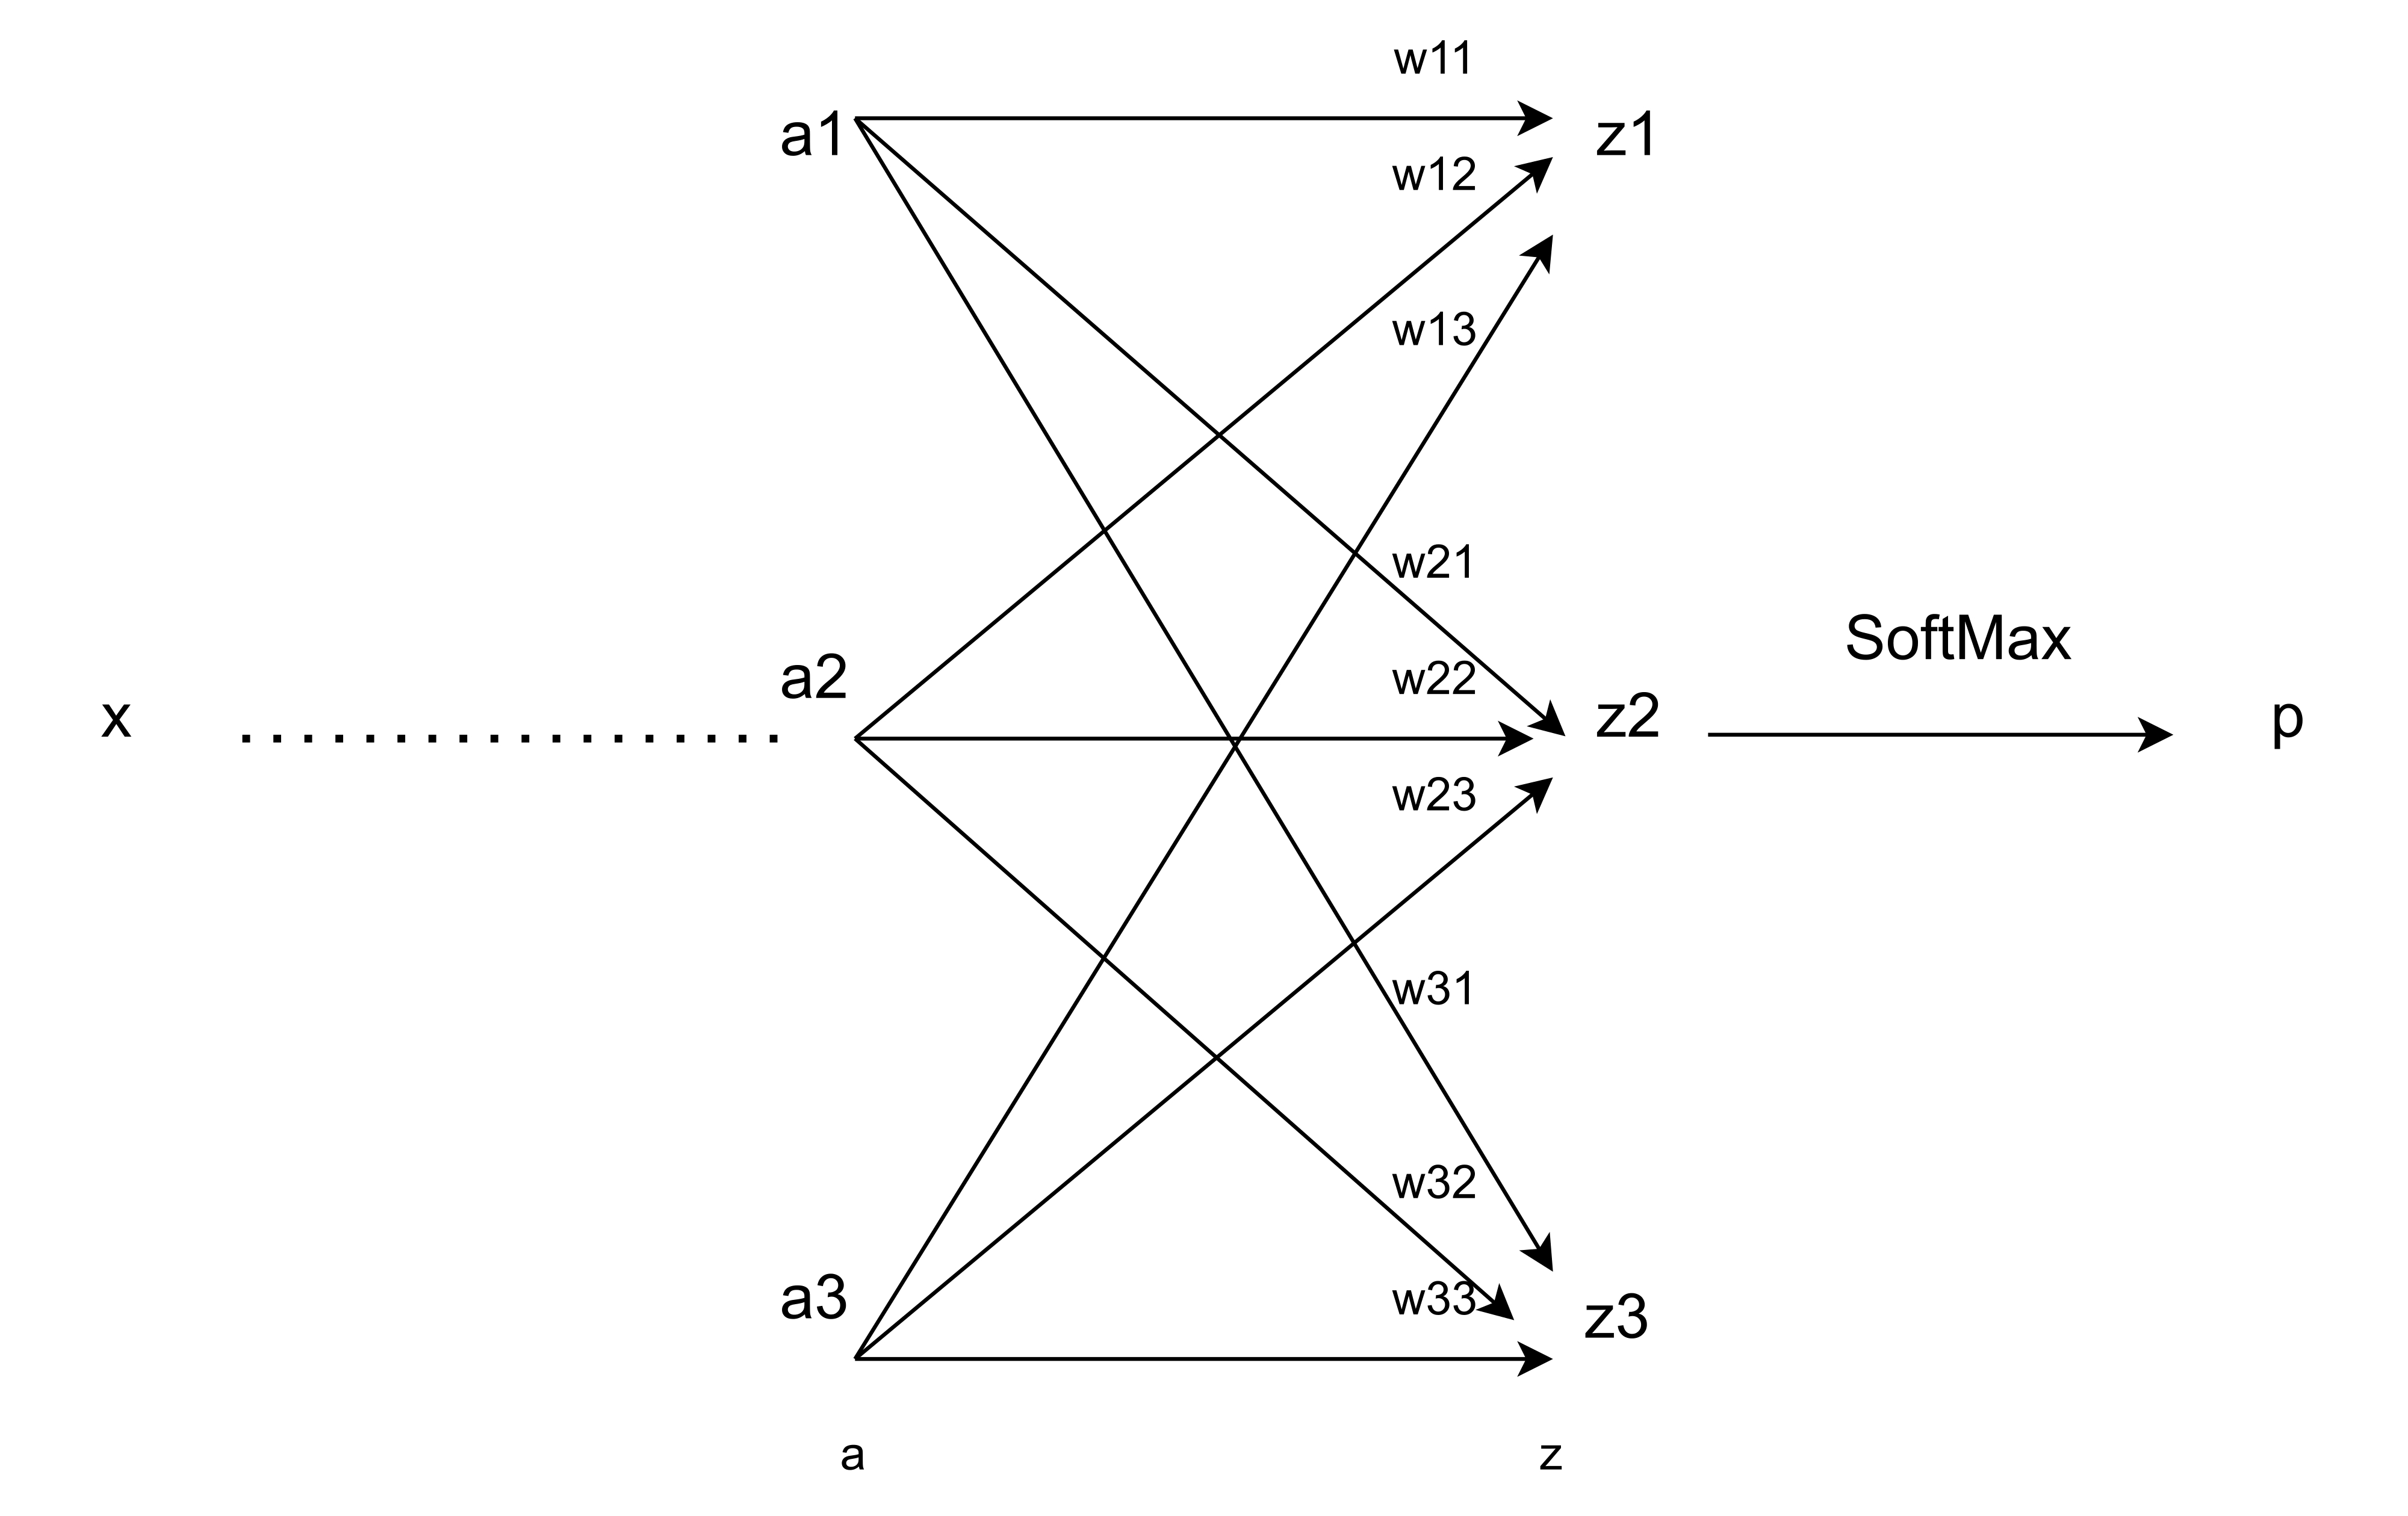
\includegraphics[scale=1.0,width=0.5\columnwidth]{simplenn.jpg}
\caption{Fully connected layer of a convolutional neural network} 
\label{fig:simplenn}
\end{figure} 




In this section, we discuss the impact of PGT on weight gradients. Let the input and
output of the last convolutional layer of a convolutional neural network be \textbf{x}
and \textbf{a} respectively (Fig. \ref{fig:simplenn}). The last layer which is a fully
connected layer, produces logits \textbf{z} by combining \textbf{a} with weights and
thereafter the network generates the predicted probability vector \textbf{p} from the
logits using softmax activation function. We note that a$_i \geq 0$ $ \forall i$  as,
\textbf{a} is the output of ReLU activation functions.


Here, $z_i = \sum_{j=1}^{C}w_{ij}a_j$, so $\frac{\partial L}{\partial w_{ij}} =
a_j\frac{\partial L}{\partial z_{i}} $. However, if we apply PGT while training the
neural network, then $\widehat{\frac{\partial L}{\partial w_{ij}}}
=a_j\widehat{\frac{\partial L}{\partial z_i}}$

If the activation of the $j^{th}$ neuron is zero, i.e. $a_j = 0$ then there is zero
gradient for all weights which acts on $a_j$ both for normal training and training with
PGT, as $a_j$ has no contribution in the computation of logits. However, the interesting
thing is to observe the effect of PGT when $a_j > 0$. As, the activation values $(a_j)$
are positive, so $ \widehat{\frac{\partial L}{\partial z_i}}  > \frac{\partial
L}{\partial z_{i}} \Rightarrow$ $\widehat{\frac{\partial L}{\partial w_{ij}}} >
\frac{\partial L}{\partial w_{ij}} \forall j \in (1,2,\ldots C)$ and similar
relationship for $a_j < 0$. With PGT, the weight updating rule for $(t+1)^{th}$
iteration then becomes,
\begin{equation}
\label{weight_update_PGT}
w_{ij}^{t+1} = w_{ij}^{t} - \eta \widehat{\frac{\partial L}{\partial w_{ij}^{t}}}
\end{equation}
The weight update equation using PGT, can also be viewed in terms of the following
equation,
\begin{equation}
\label{weight_update_final_PGT}
w_{ij}^{t+1} = w_{ij}^{t} - \frac{\eta}{C_{PGT}} \frac{\partial L}{\partial w_{ij}^{t}}
\end{equation}

For neural networks, the exponential nature of the softmax function produces sharp
distribution for predicted probability vector. For example, if \textbf{z} is $[20, 30,
10]$ then \textbf{p} is equal to $[4\times 10^{-5},  0.99995, 2\times10^{-9}]$. When the
network is at the initial phase of training, most of the training examples are
misclassified. Under this scenario, PGT helps to update the weights in a better manner
than traditional gradients. Suppose the label vector \textbf{q} is $[1, 0, 0]$ then it
indicates that $z_1$ is the logit corresponding to ground truth class and $z_2$ is the
logit where the network has assigned the highest probability. Similarly, $z_3$ is the
logit where the network has assigned a low probability as well as the label vector is
also $0$ for this logit. Here $\frac{\partial L}{\partial w_{1j}^{t}} = \epsilon a_j > 0
\Rightarrow$ $ \widehat{\frac{\partial L}{\partial w_{1j}^{t}}} < \frac{\partial
L}{\partial w_{1j}^{t}} \Rightarrow C_{PGT} > 1$ $\forall j \in (1, 2,\ldots C)$.
Advanced gradient updation algorithms like AdaGrad \cite{duchi2011adaptive} reduces the
gradient in the direction where the directional derivative for a weight is high. It
reduces the learning rate for the weight so that the gradient in that direction is not
too large in order to make the update process less volatile. The formulation of PGT also
implicitly reduces the partial derivative in the same manner for the high derivative
directions, the only difference with the AdaGrad is that $C_{PGT}$ depends only on the
current iteration's gradient and not on previous iterations like AdaGrad. Similarly we
can observe that for this example, $\frac{\partial L}{\partial w_{3j}^{t}} = \delta a_j
\approx 0 \Rightarrow$ $  \widehat{\frac{\partial L}{\partial w_{3j}^{t}}} >
\frac{\partial L}{\partial w_{3j}^{t}} \Rightarrow C_{PGT} < 1$ $\forall j \in (1,
2,\ldots C)$. As directional derivative for the weights associated with third logit is
extremely low, PGT helps to increase the derivative in these directions so that the
training process does not become too slow.

\subsection{Effect of PGT on class separation}
\label{sec:pgt_class_separation}

During final iterations of training, we analyze the iteration-wise gradient behaviour
where the network assigns the highest probability to the correct class for a given
training example; we deduce the effects of PGT in the next immediate training iteration.
For example, if \textbf{z} is $[30, 20, 10]$ then \textbf{p} is $[0.99995, 4\times
10^{-5}, 2\times10^{-9}]$ and \textbf{q} is $[1, 0, 0]$. There is no change in the
weight update due to PGT when $a_j = 0$. However, when $i \neq 1$ and $a_j > 0$,
$|\widehat{\frac{\partial L}{\partial w_{1j}^{t}}}| > |\frac{\partial L}{\partial
w_{1j}^{t}}|$ and $\widehat{\frac{\partial L}{\partial w_{ij}^{t}}} > \frac{\partial
L}{\partial w_{ij}^{t}}$. Here in this example $\frac{\partial L}{\partial z_{1}^{t}} <
0 \Rightarrow \frac{\partial L}{\partial w_{1j}^{t}} < 0 \Rightarrow$
$\widehat{w_{1j}^{t+1}} > w_{1j}^{t+1} > w_{1j}^{t} \forall j$. We also know that
$z_i^{t+1} = \sum_{j=1}^{C}w_{ij}^{t+1}a_j$ and $\widehat{z_i^{t+1}} =
\sum_{j=1}^{C}\widehat{w_{ij}^{t+1}}a_j$. It indicates that $\widehat{z_{1}^{t+1}} >
z_{1}^{t+1} > z_{1}^{t}$ as all the weights associated with first logit is larger while
using PGT in $(t+1)^{th}$ iteration. Similarly, for the non-true classes
$\widehat{w_{ij}^{t+1}} < w_{ij}^{t+1} < w_{ij}^{t}$ when $i \neq 1$ $\forall j$ as
$\frac{\partial L}{\partial z_{i}^{t}} > 0$. So in $(t+1)^{th}$ iteration,
$\widehat{z_{i}^{t+1}} < z_{i}^{t+1} < z_{i}^{t}$ when $i \neq 1$. We observe that
$dist(\widehat{z_{1}^{t+1}}, \widehat{z_{i}^{t+1}}) > $  $dist(z_{1}^{t+1},
z_{i}^{t+1})$ where the first logit corresponds to the true class and all other logits
indexed by $i$ are non-true classes. Therefore the distance between correct and
incorrect class logits increases due to PGT and this leads to better class separation.

\clearpage

\subsection{Sample Code}

In PyTorch, the available method to modify gradients in the backward pass is using the
\codeword{register_hook} function which is called in the \codeword{forward} function.

\begin{figure}[ht] \hrule \lstinputlisting[language=Python]{code.py} \hrule
\vspace{0.25cm} \caption{Python code of PowerGrad Transform based on PyTorch. }
\label{fig:code}
\end{figure}



\clearpage

\subsection{Grid search for different values of $\alpha$}


\begin{figure}[ht]
\centering
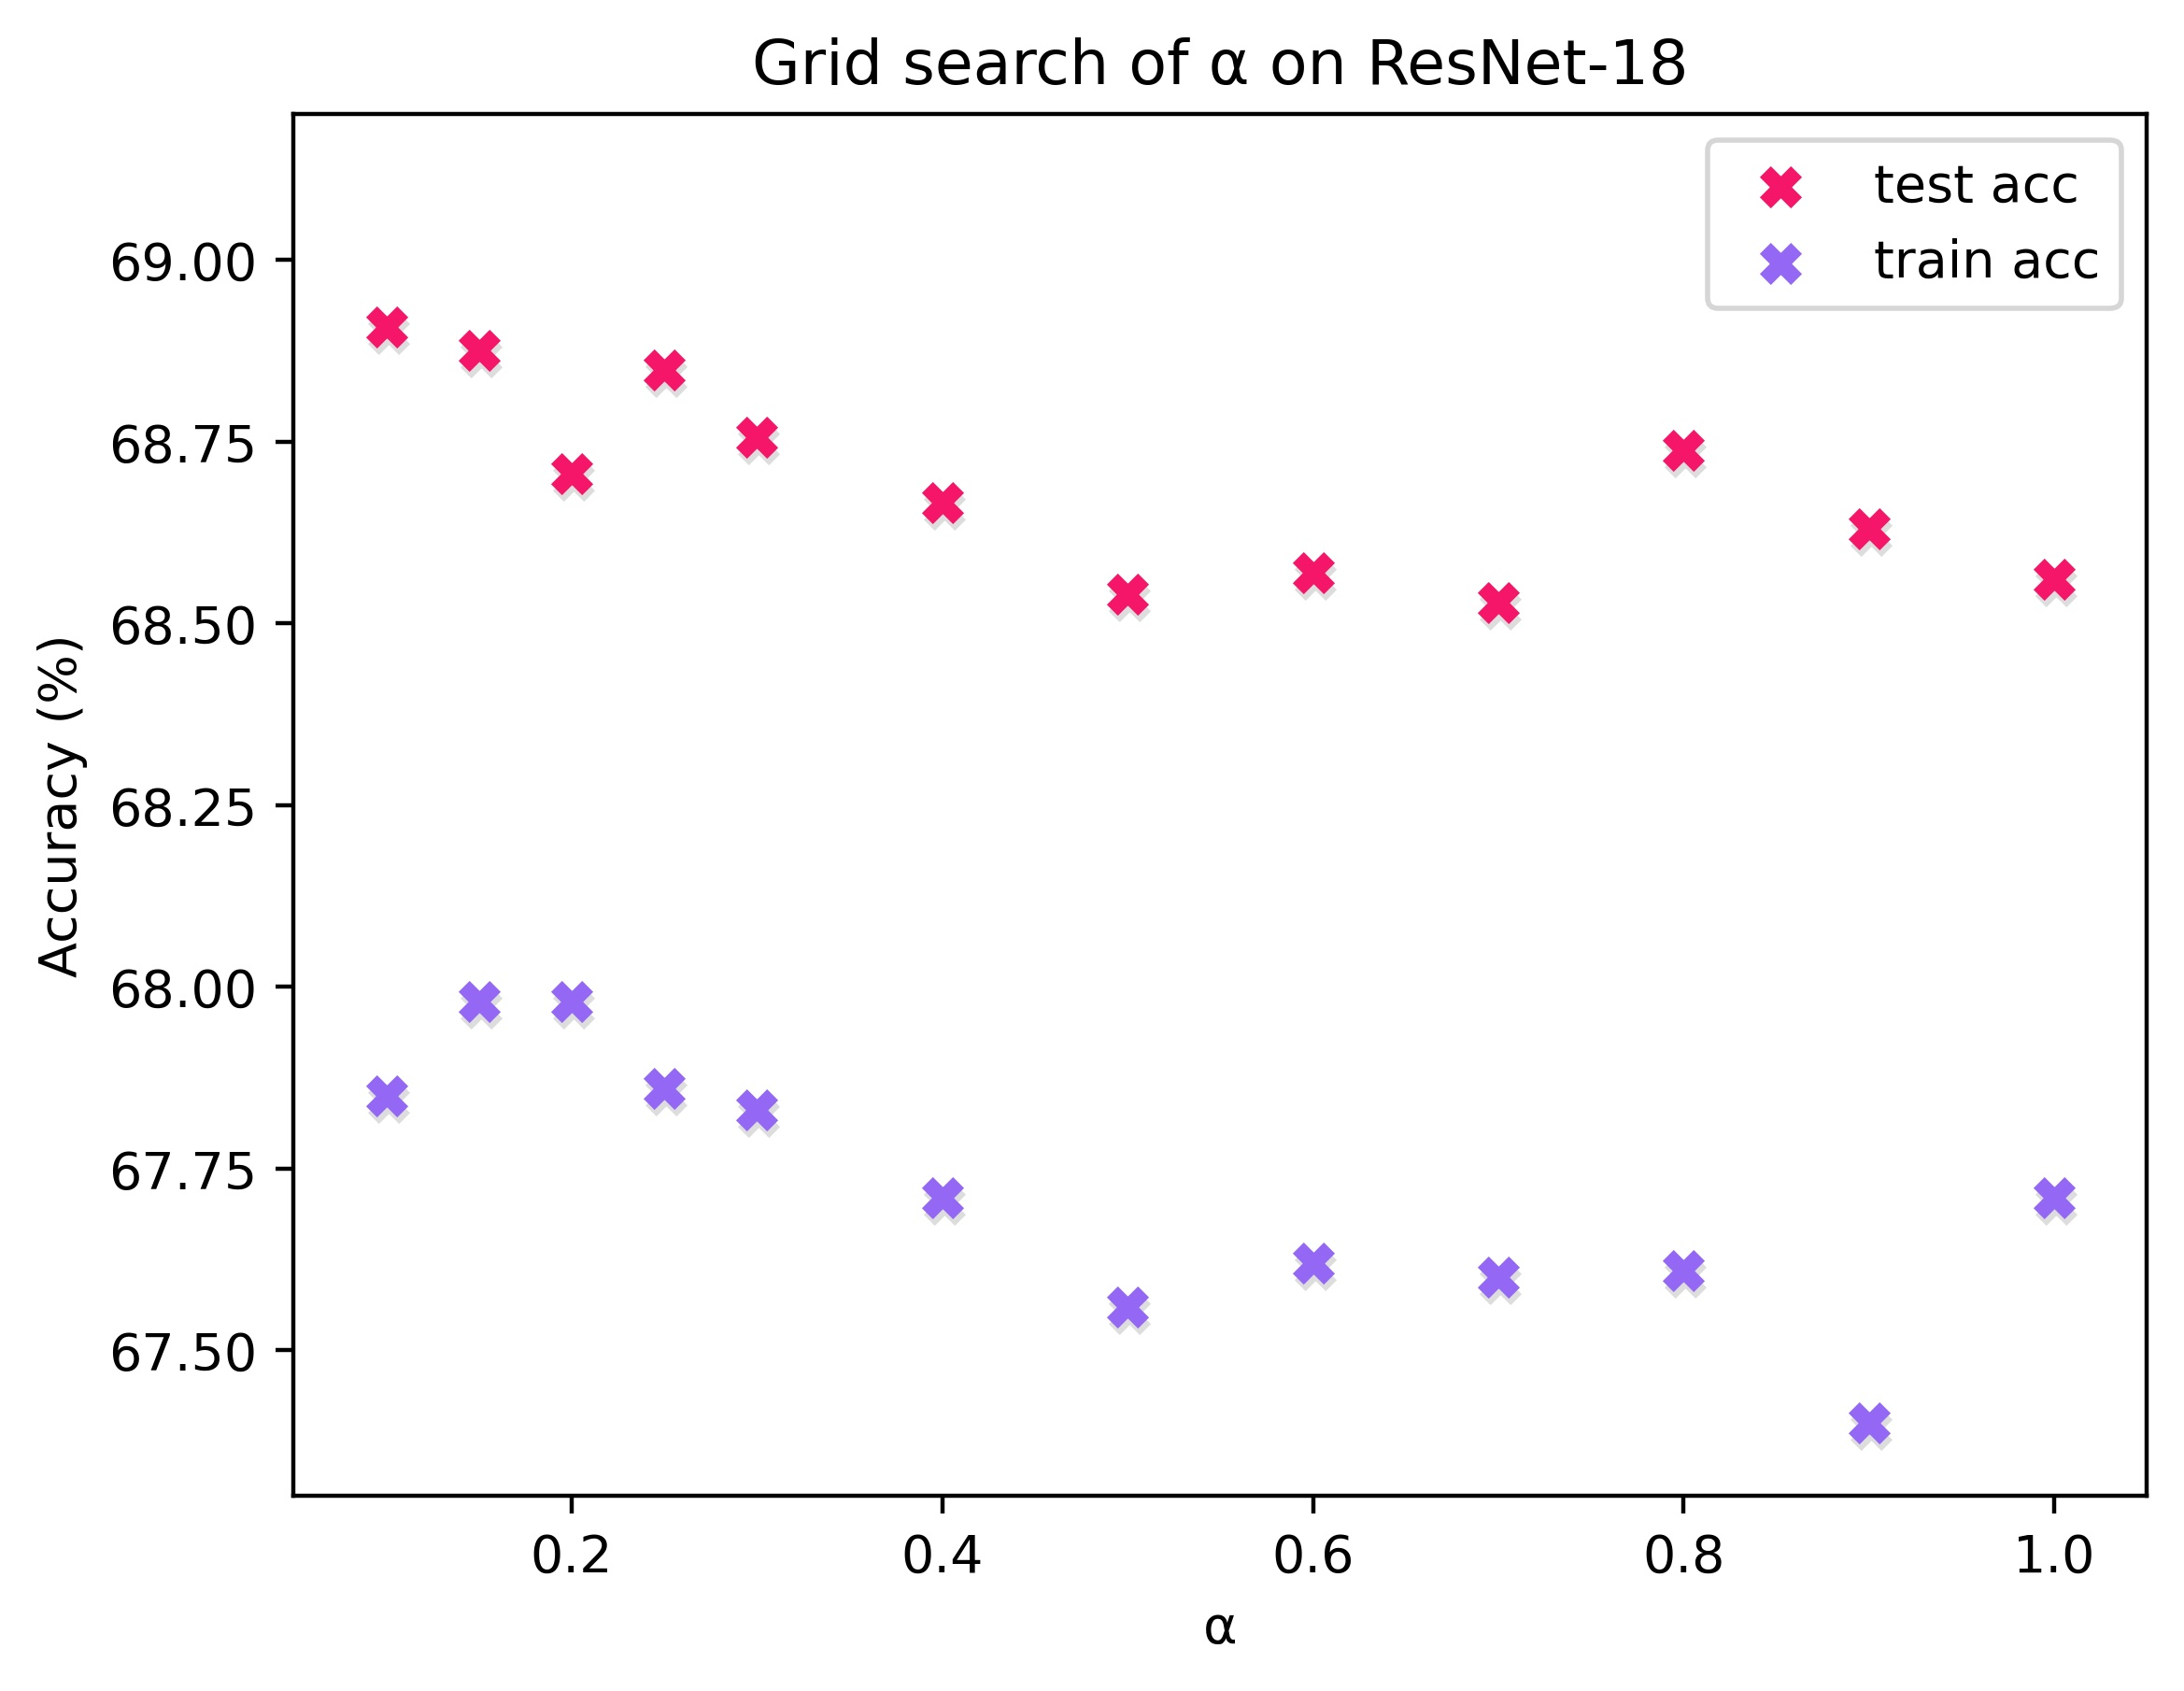
\includegraphics[width=0.5\columnwidth]{r18_grid_search}
\caption{ Grid search for various values of $\alpha$ for ResNet-18 architecture with the
ImageNet dataset. Each datapoint is collected over a 50 epoch budget, with other
hyperparameters kept the same as mentioned in section \ref{sec:Expe}. }
\label{fig:grid_searcha}
\end{figure}


\begin{figure}[ht]
\centering
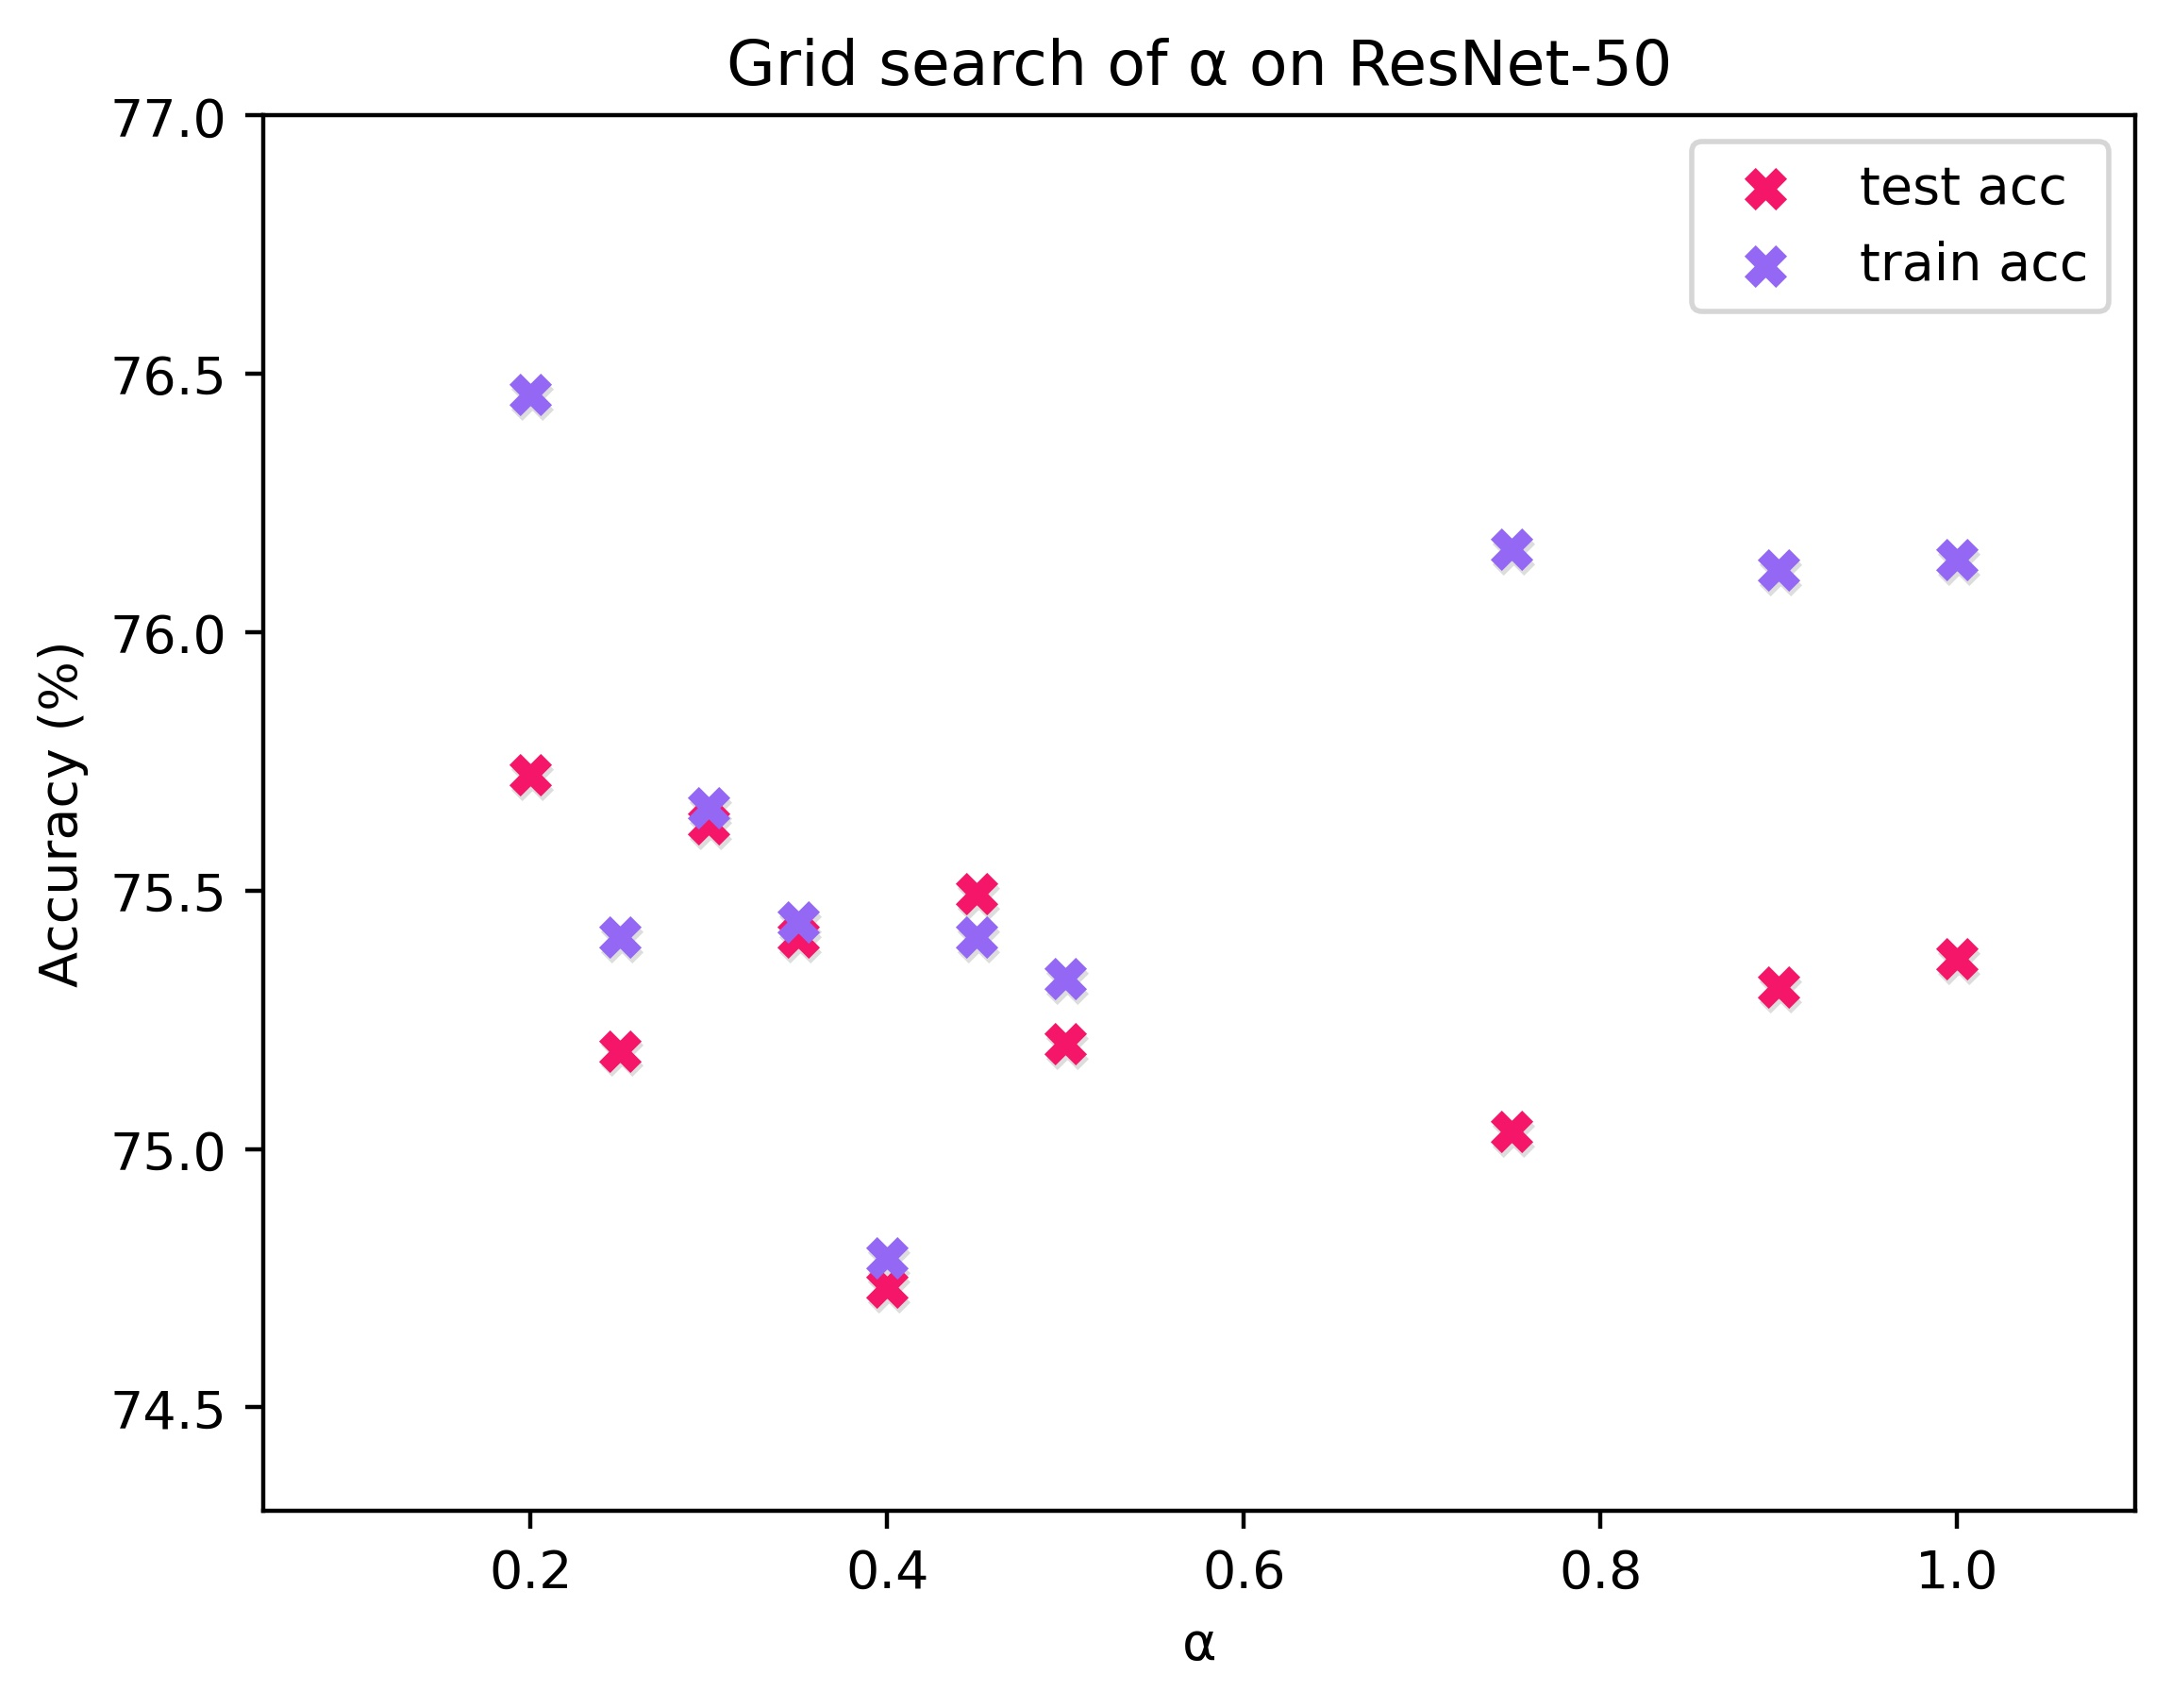
\includegraphics[width=0.5\columnwidth]{r50_grid_search}
\caption{ Grid search for various values of $\alpha$ for ResNet-50 architecture with the
ImageNet dataset. Each datapoint is collected over a 50 epoch budget, with other
hyperparameters kept the same as mentioned in section \ref{sec:Expe}. }
\label{fig:grid_searchb}
\end{figure}


\clearpage



\begin{figure}[ht]
\centering
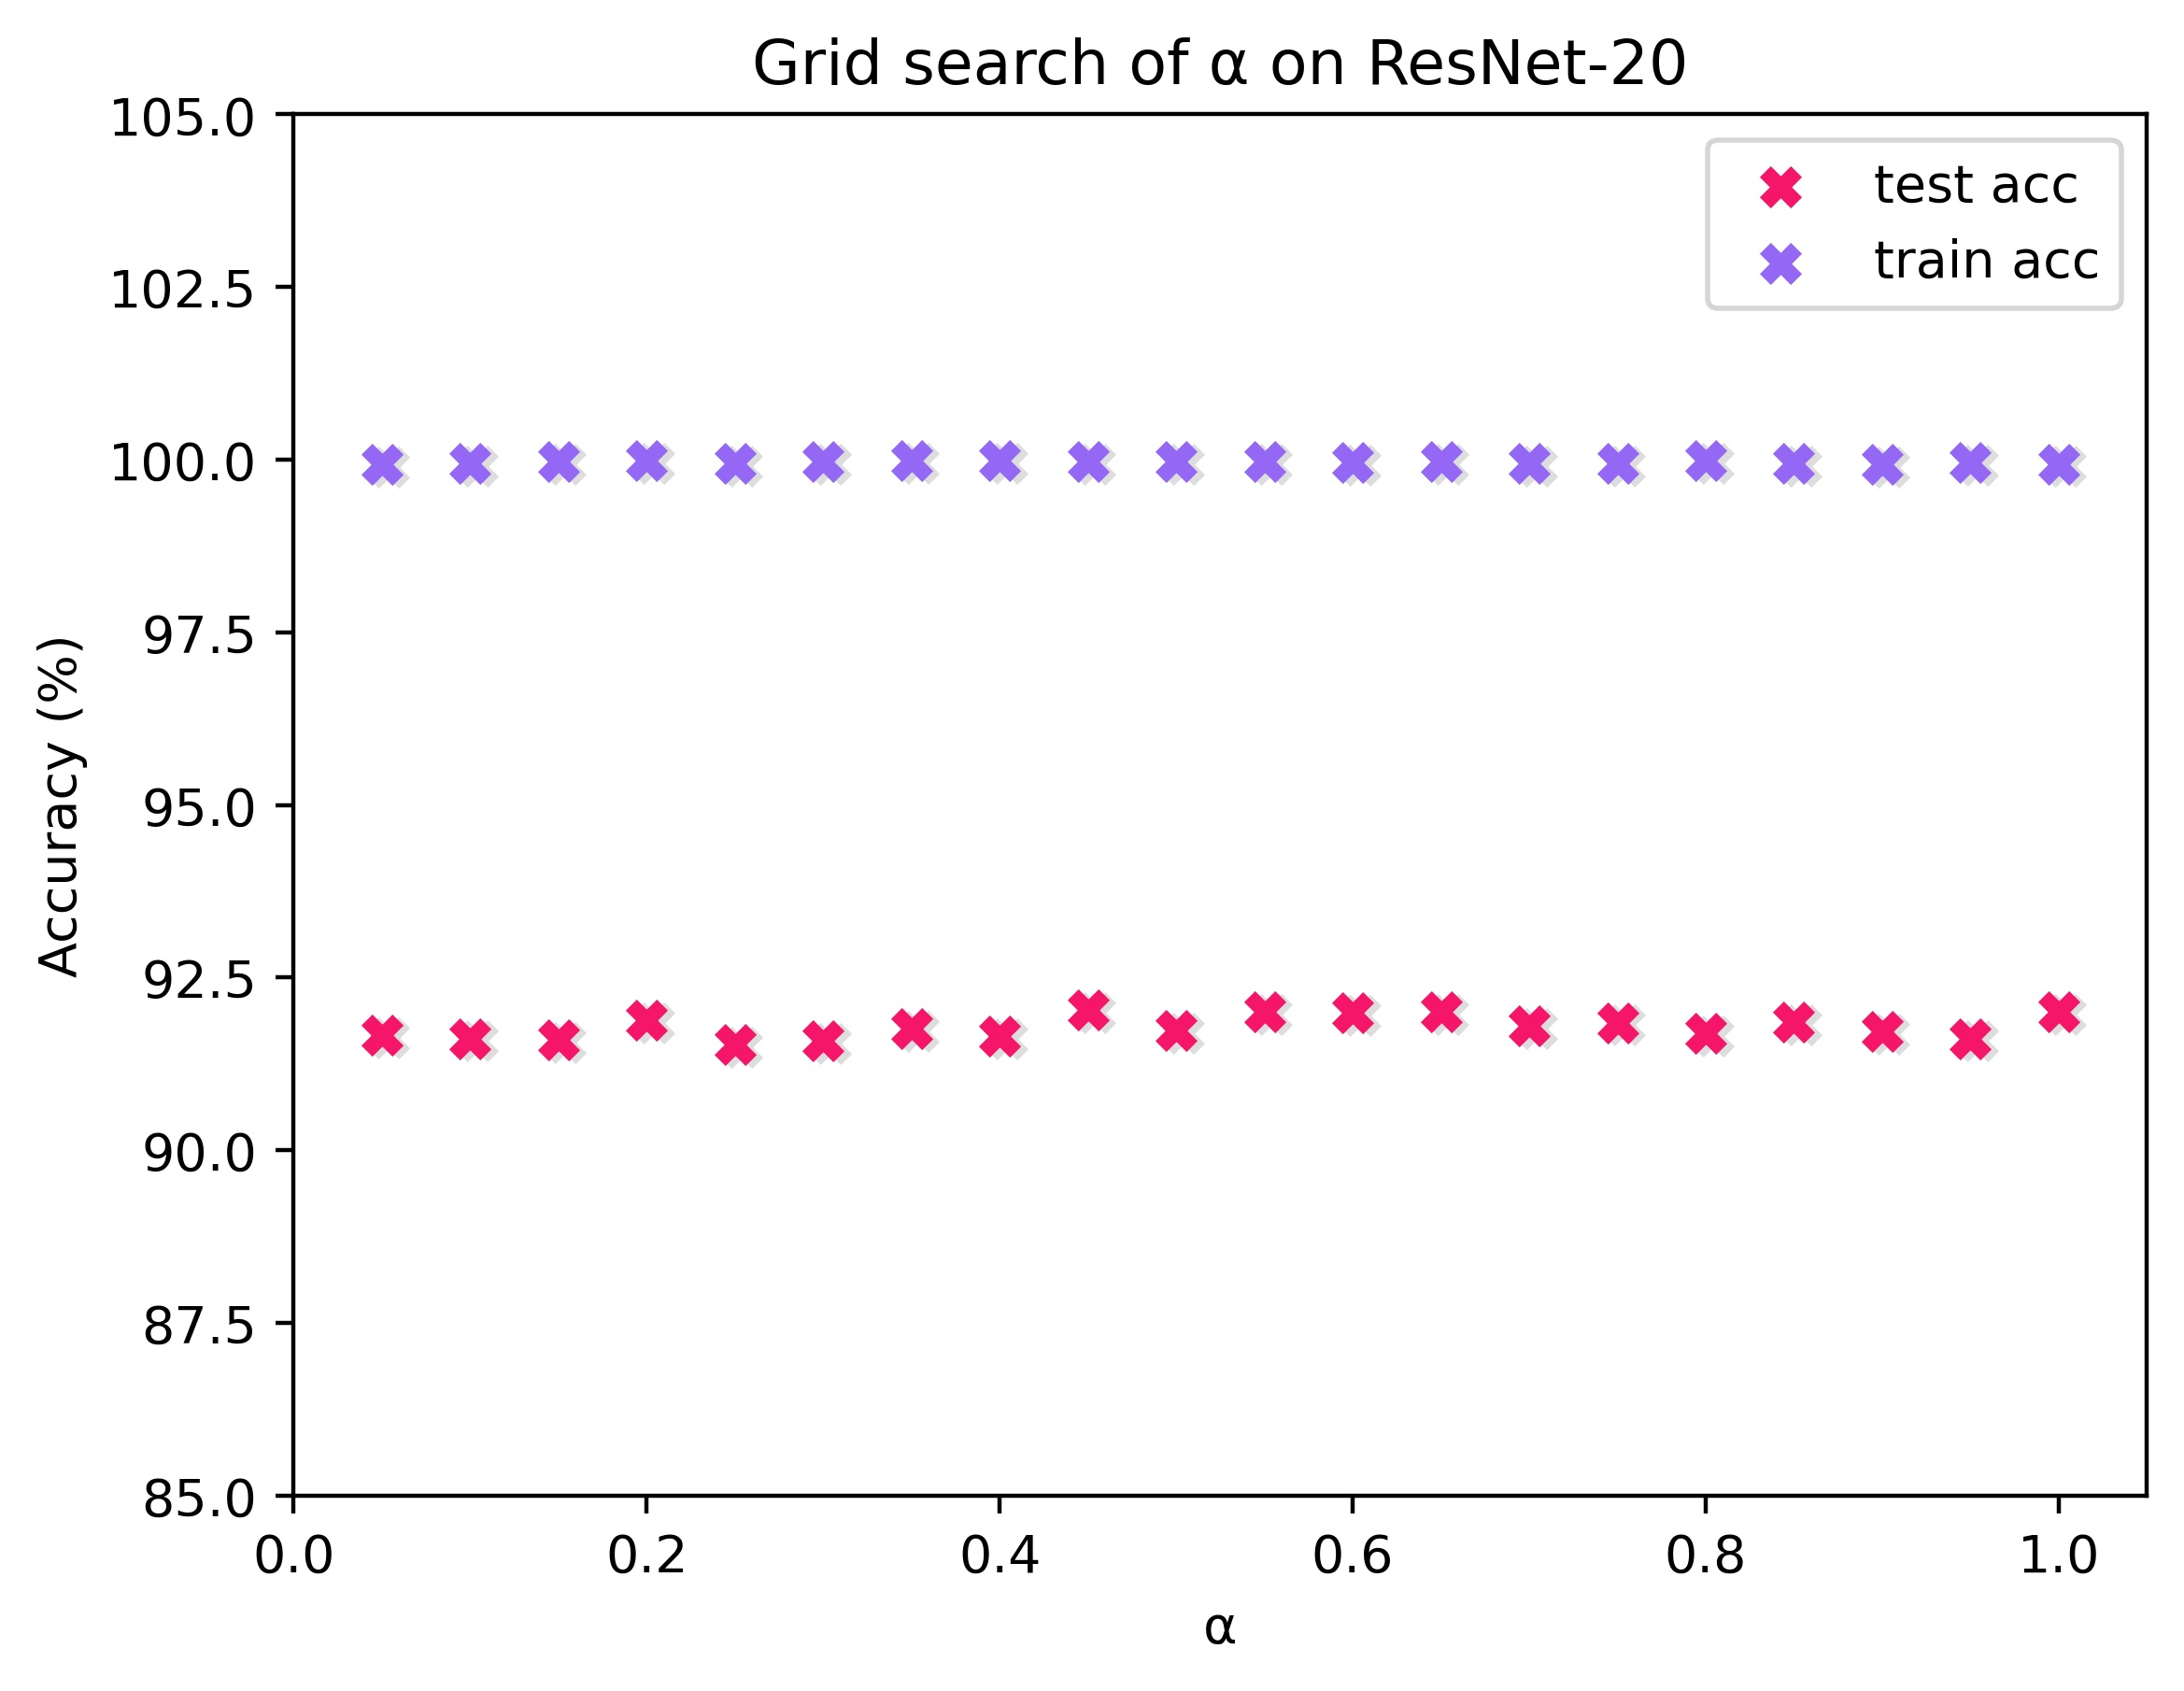
\includegraphics[width=0.5\columnwidth]{cifar10_grid_search}
\caption{\\ResNet-20 CIFAR-10}
\caption{ Grid search for various values of $\alpha$ for ResNet-20 architecture with the
CIFAR-10 dataset. Each datapoint is collected over a 360 epoch budget. }
\label{fig:grid_searchc}
\end{figure}


There is no effect of PGT on small datasets such as CIFAR-10. In these scenarios,
networks almost always achieve $100\%$ training accuracy, leaving no room for PGT to
assist.



\clearpage

\subsection{Norm plots of weights (baseline (low batch size)) of non-BN ResNet-18}
\label{sec:plots1}
\begin{figure}[ht]
\centering
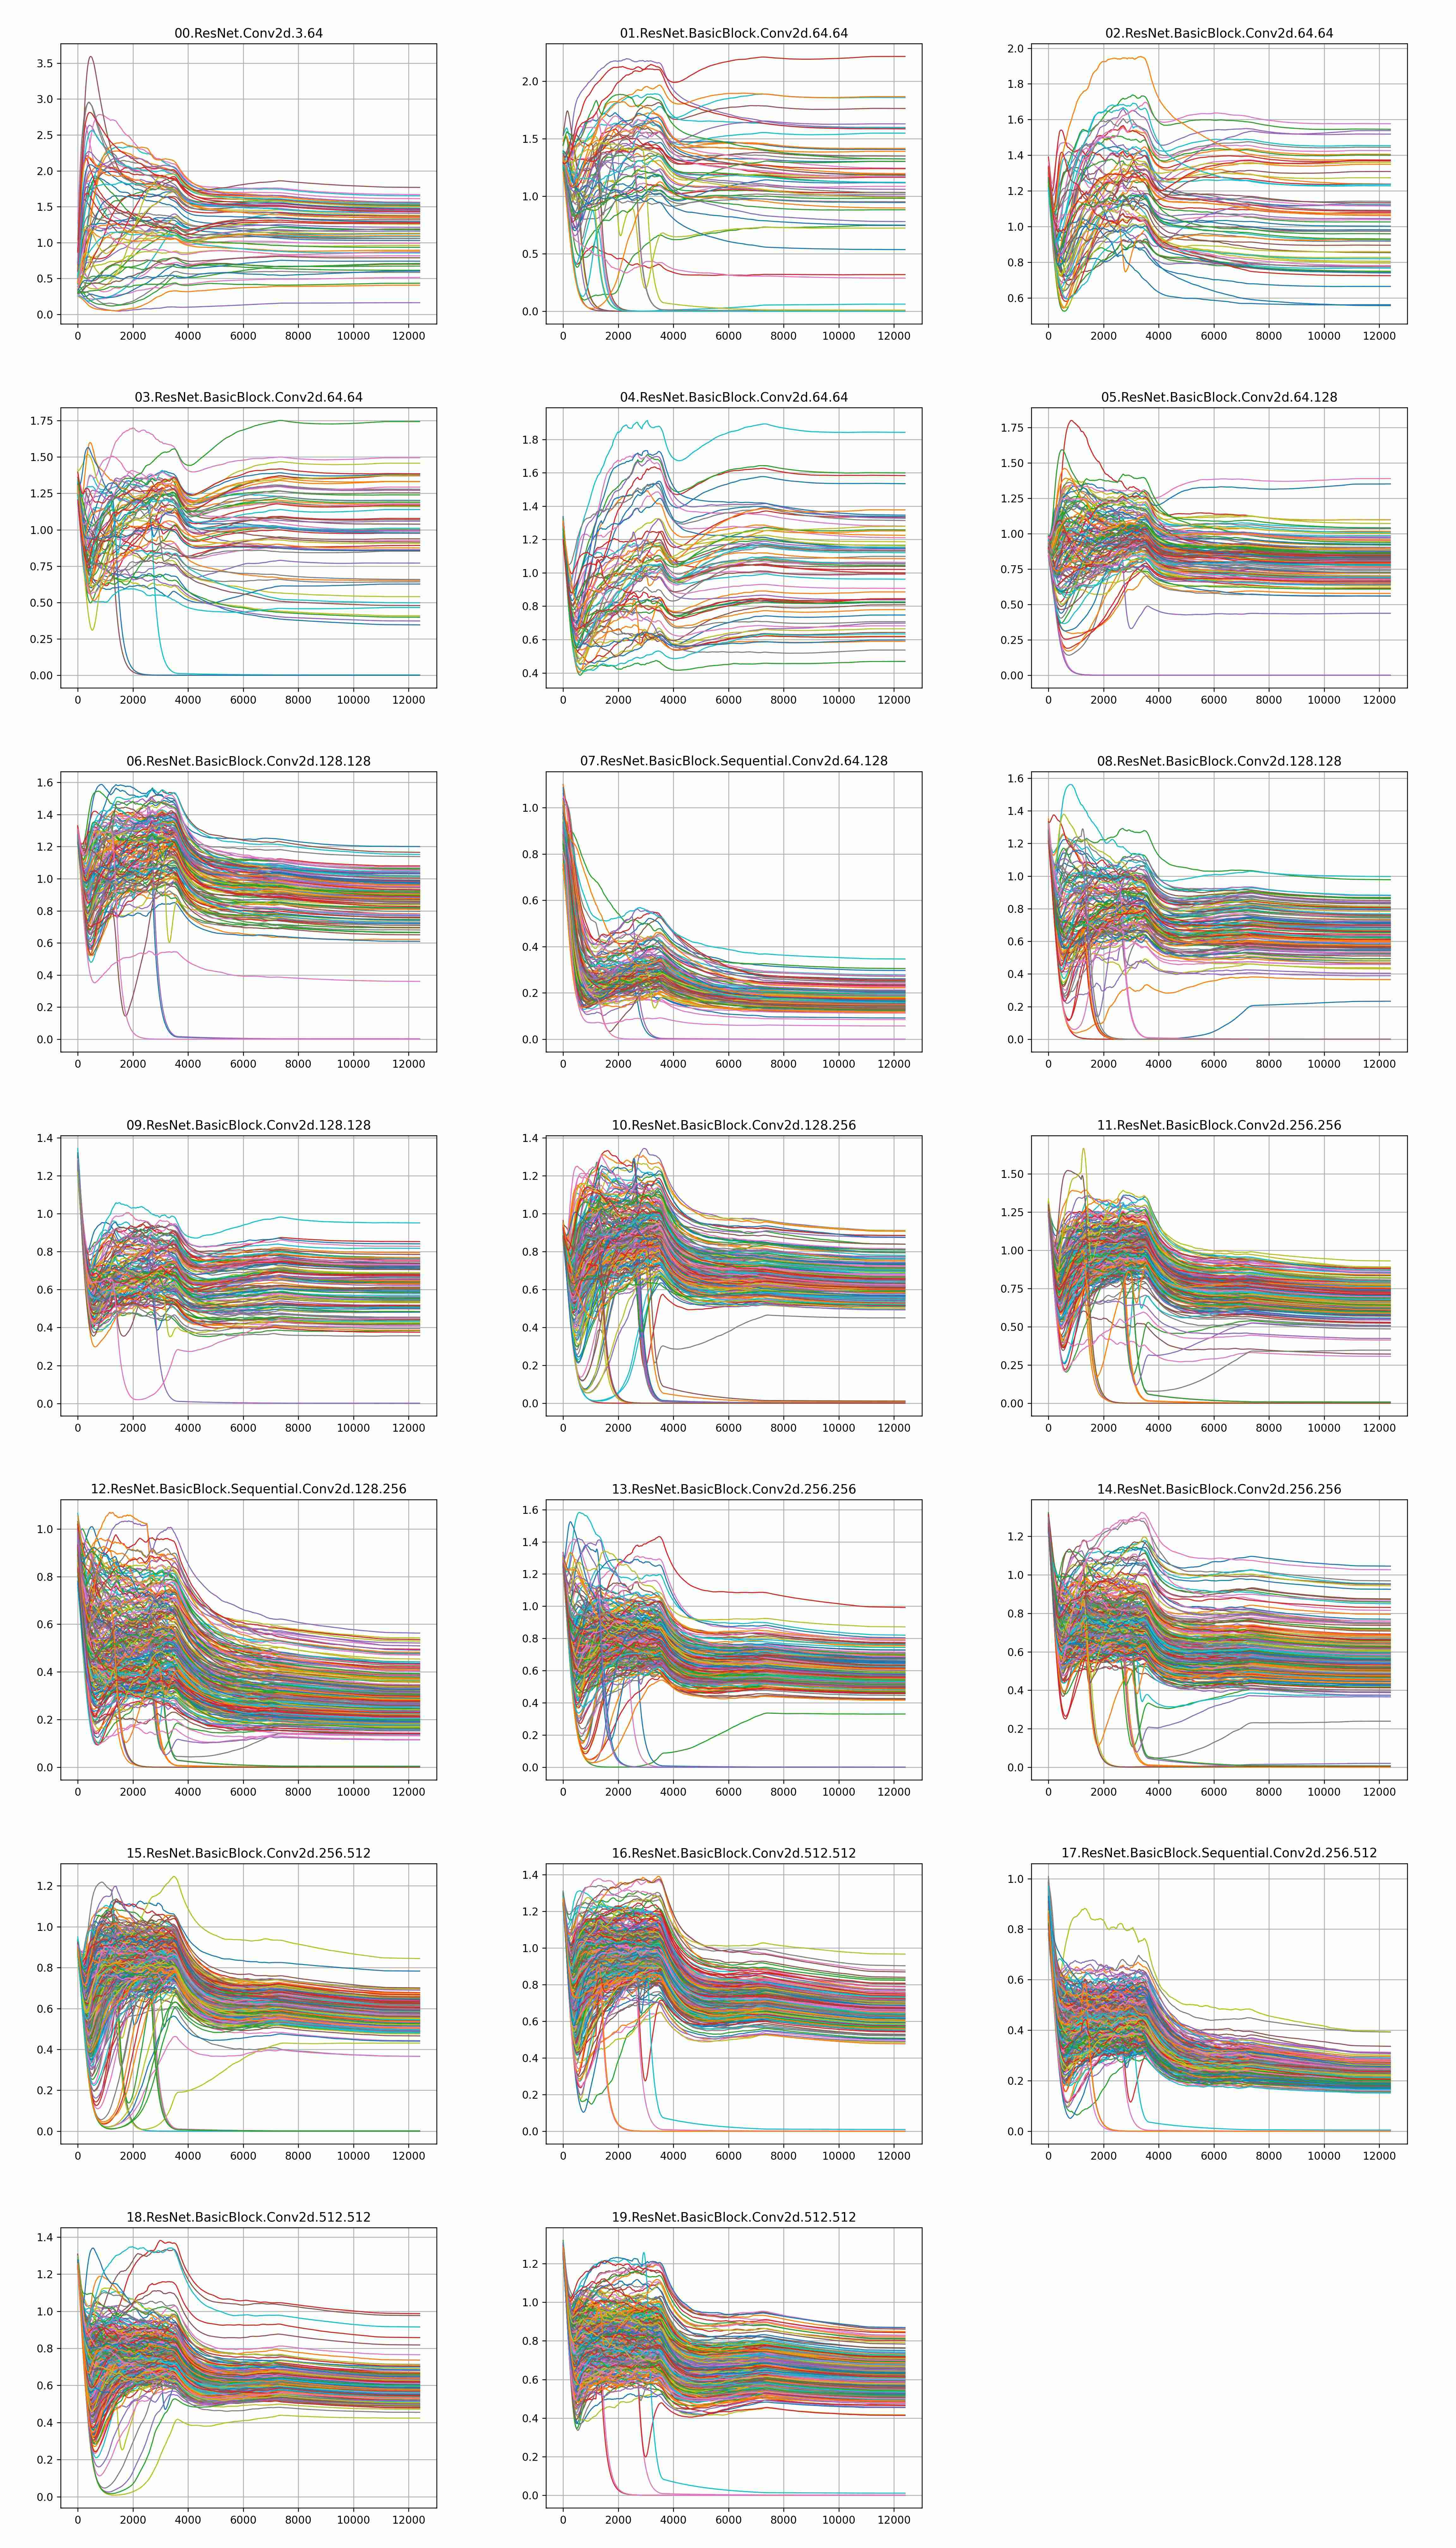
\includegraphics[width=0.57\textwidth]{compressed/baseline-w_norm}
\caption{ Method: baseline, batch size = 256. This is a plot depicting the
iteration-wise evolution of the norm of each filter in each layer. Each subplot
corresponds to a layer of the unnormalized ResNet-18. Above each subplot, the layer
indices are shown. Each filter in each subplot is shown with a separate and randomly
determined colour. Readers are requested to zoom in. } 
\end{figure}

\clearpage

\subsection{Norm plots of weights (baseline (high batch size)) of non-BN ResNet-18}
\label{sec:plots2}
\begin{figure}[ht]
\centering
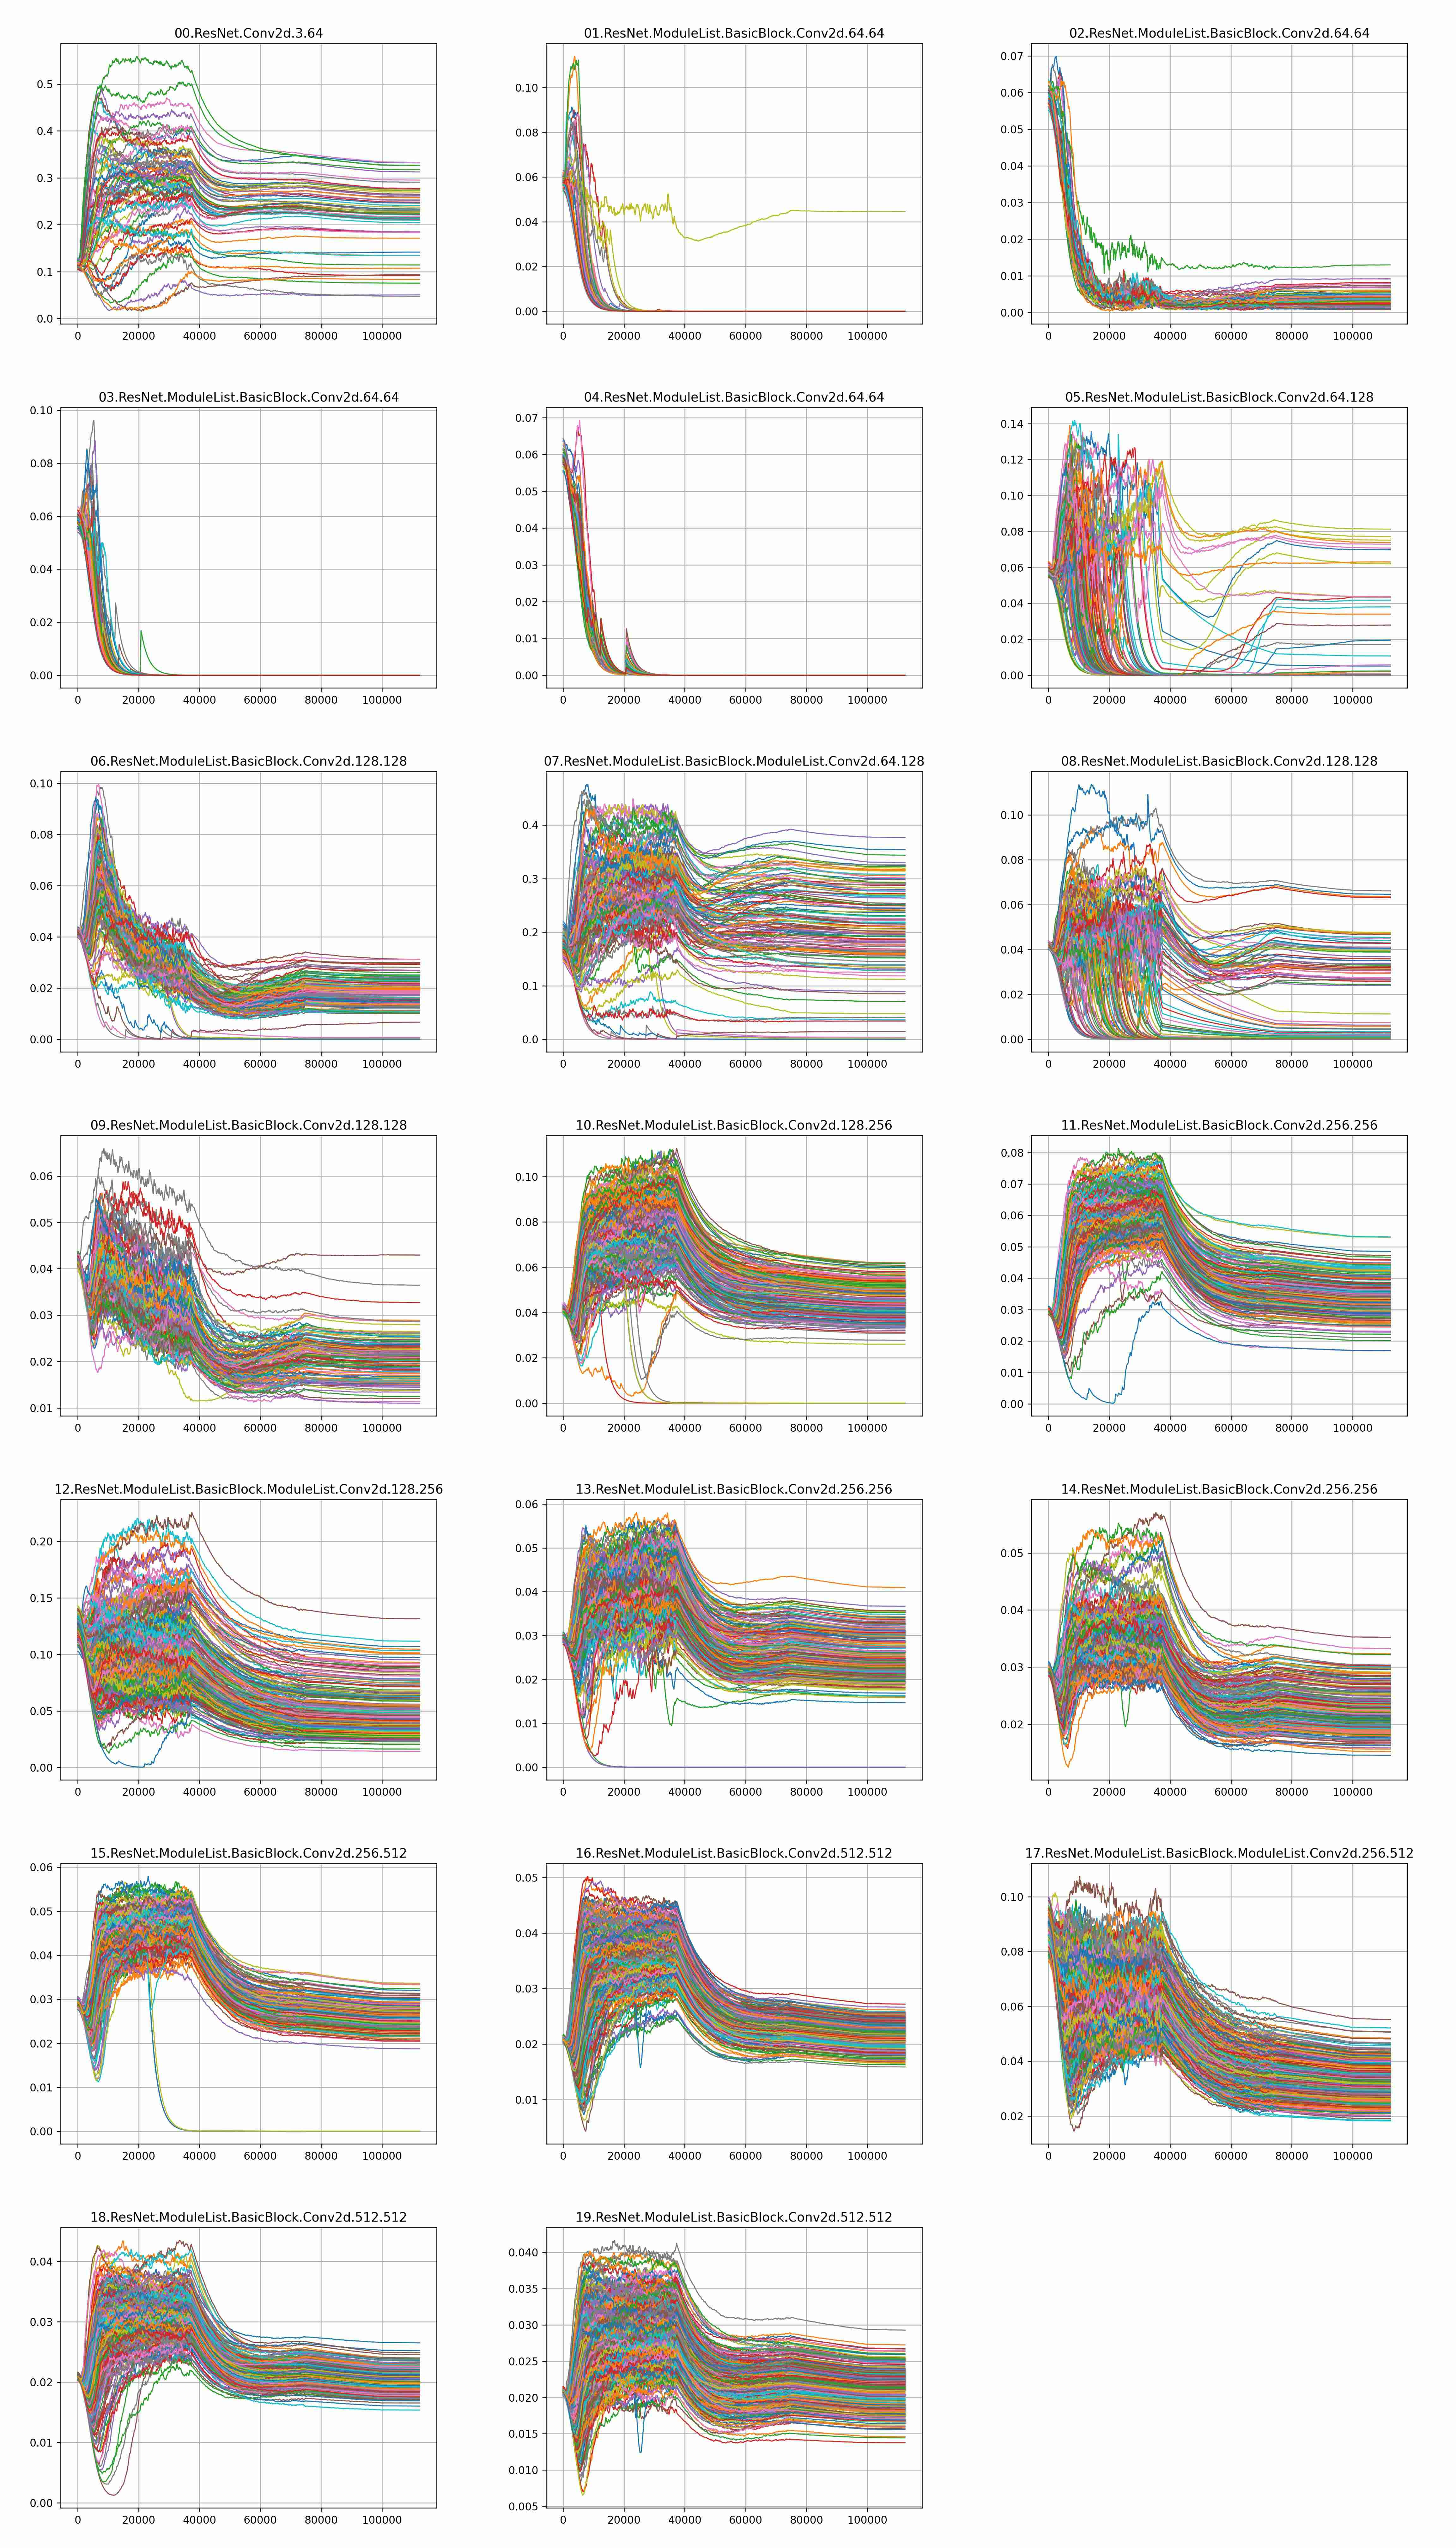
\includegraphics[width=0.57\textwidth]{compressed/baseline_high_bs-w_norm}
\caption{ Method: baseline (high batch size), batch size = 1024. This is a plot
depicting the iteration-wise evolution of the norm of each filter in each layer. Each
subplot corresponds to a layer of the unnormalized ResNet-18. Above each subplot, the
layer indices are shown. Each filter in each subplot is shown with a separate and
randomly determined colour. Readers are requested to zoom in. } \end{figure}

\clearpage

\subsection{Norm plots of weights (PGT) of non-BN ResNet-18}
\label{sec:plots3}
\begin{figure}[ht]
\centering
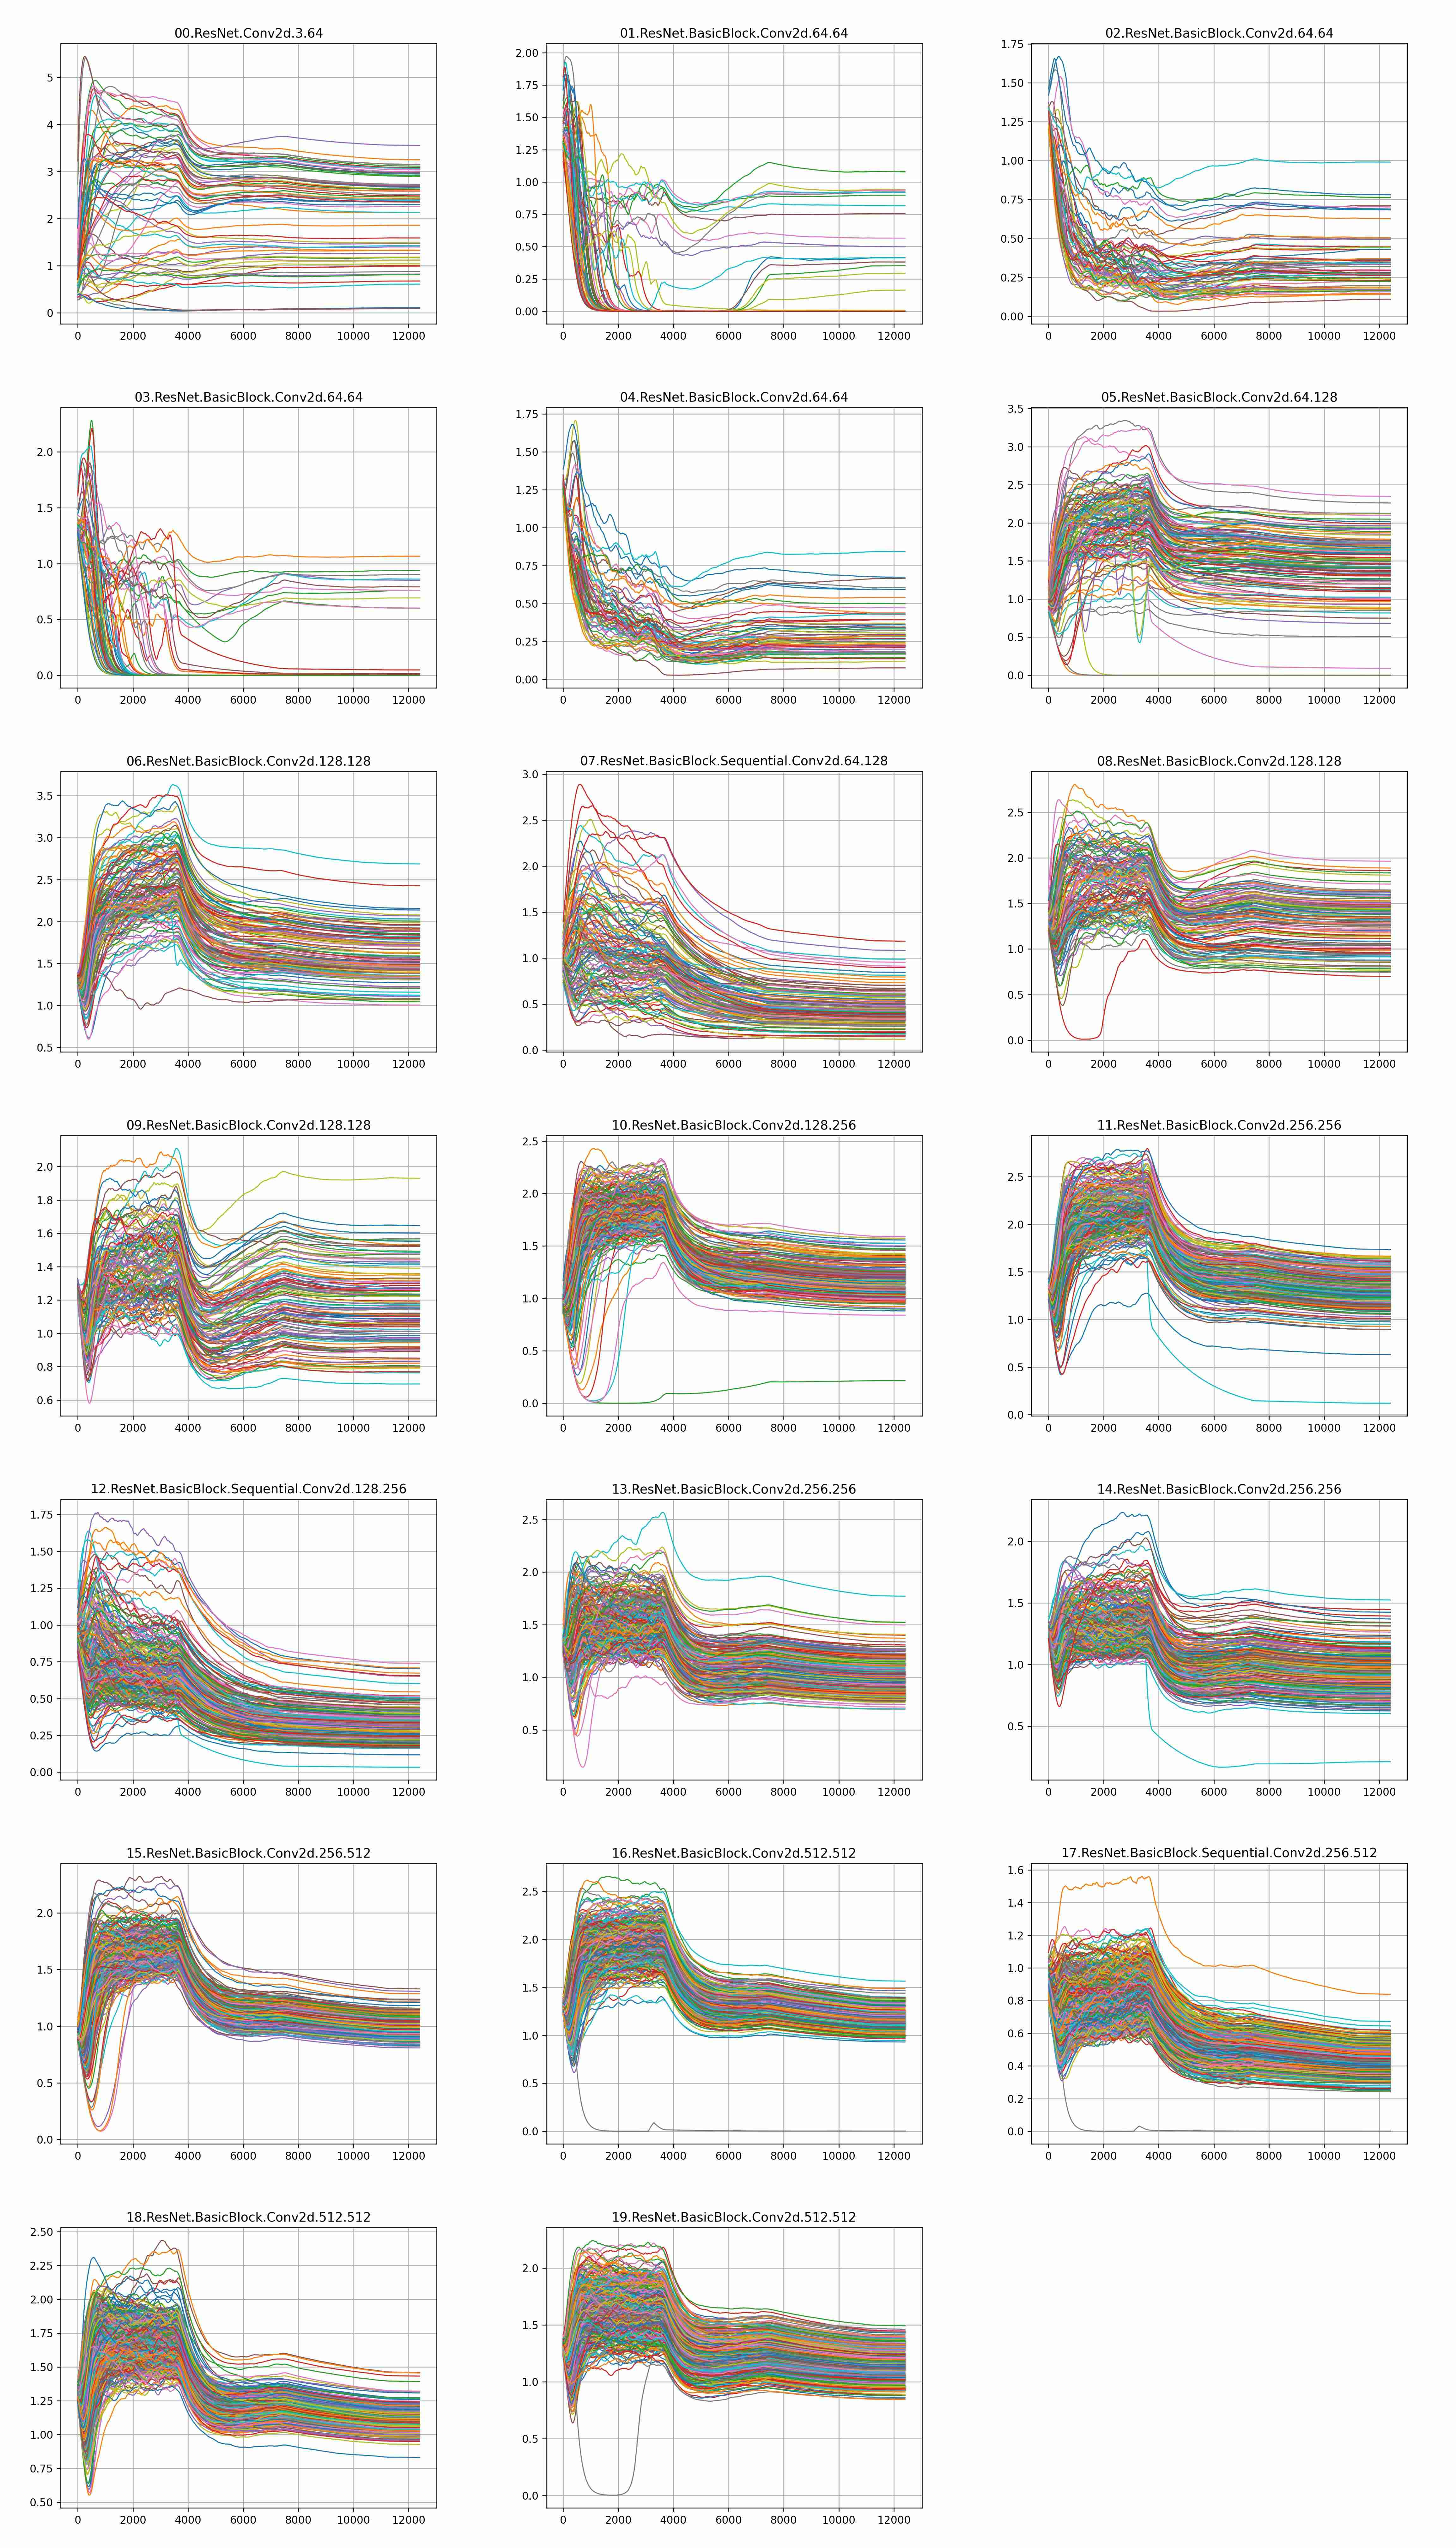
\includegraphics[width=0.57\textwidth]{compressed/pgt-w_norm}
\caption{ Method: PGT, batch size = 256. This is a plot depicting the iteration-wise
evolution of the norm of each filter in each layer. Each subplot corresponds to a layer
of the unnormalized ResNet-18. Above each subplot, the layer indices are shown. Each
filter in each subplot is shown with a separate and randomly determined colour. Readers
are requested to zoom in. }
\end{figure}

\clearpage

\subsection{Norm plots of weights (AGC + PGT) of non-BN ResNet-18}
\label{sec:plots4}
\begin{figure}[ht]
\centering
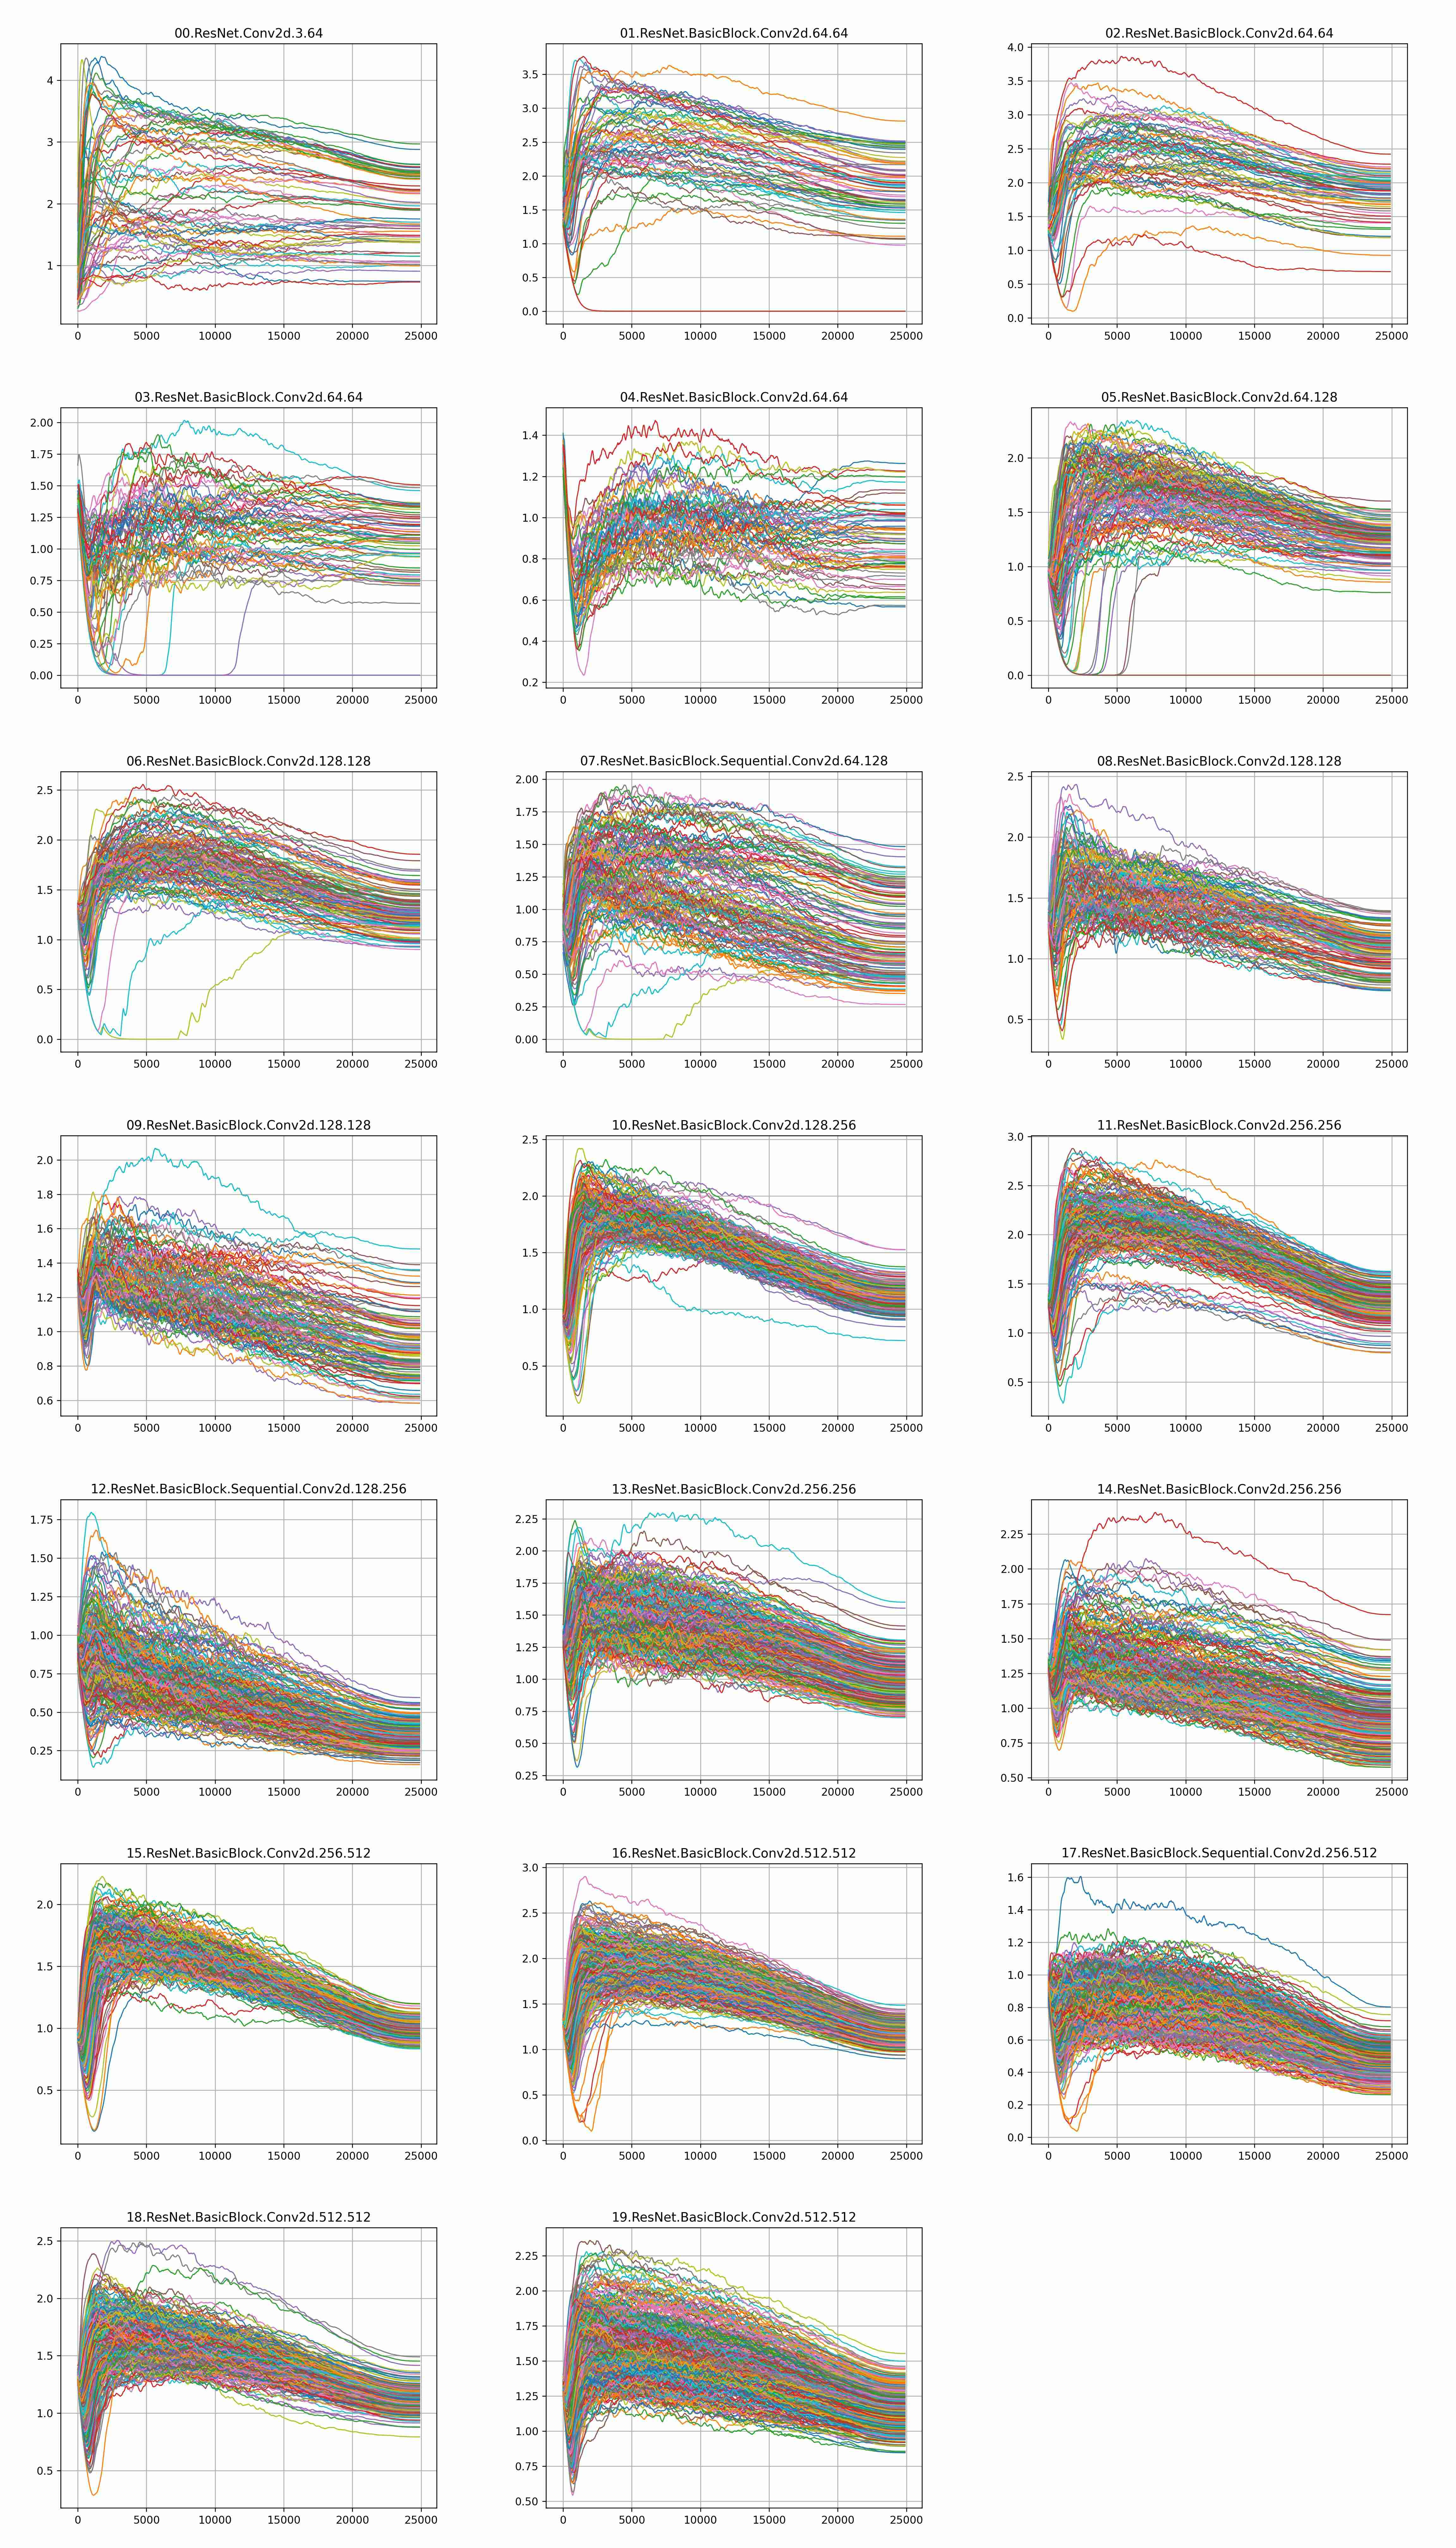
\includegraphics[width=0.57\textwidth]{compressed/agc_pgt-w_norm}
\caption{ Method: AGC + PGT, batch size = 256. This is a plot depicting the
iteration-wise evolution of the norm of each filter in each layer. Each subplot
corresponds to a layer of the unnormalized ResNet-18. Above each subplot, the layer
indices are shown. Each filter in each subplot is shown with a separate and randomly
determined colour.
Readers are requested to zoom in. }
\end{figure}



\clearpage

\subsection{ResNet-18 Layer Index Diagram}
\label{sec:r18_layers}

For the layer indices used in figures Fig. \ref{fig:norm_plots}, \ref{fig:norm_plots},
we provide a block diagram depicting the different convolutional layers of ResNet-18
with corresponding layer indices in Fig. \ref{fig:resnet18}. Each layer represents a
convolutional layer, with the layer index and the number of filters denoted alongside
it. Downsampling convolutional layers in skip connections are drawn and their layer
indices are shown on the skip connection paths.


ResNet-18 is composed of $20$ convolutional layers and one fully connected (FC) layer.
At the input, it has a single convolutional layer with filters of size $7\times 7$.
Three convolutional layers are placed in the downsampling skip connections. The
remaining convolutional layers have several $3\times 3$ filters that are grouped
together to create a block. Each basic block is connected by a skip connection. At the
end of all convolutional layers, a global average pooling layer downsamples the features
to a fixed-size feature vector and transfers it to the FC layer, which fits the features
using regression and outputs logits. The logits $z_i$ produced by the FC layer are fed
into a softmax layer, which transforms them to predicted probabilities $p_i$ using the
equation $p_i=\frac {e^{z_i}}{\sum _j e^{z_j}}$.


\begin{figure}[ht] \centering 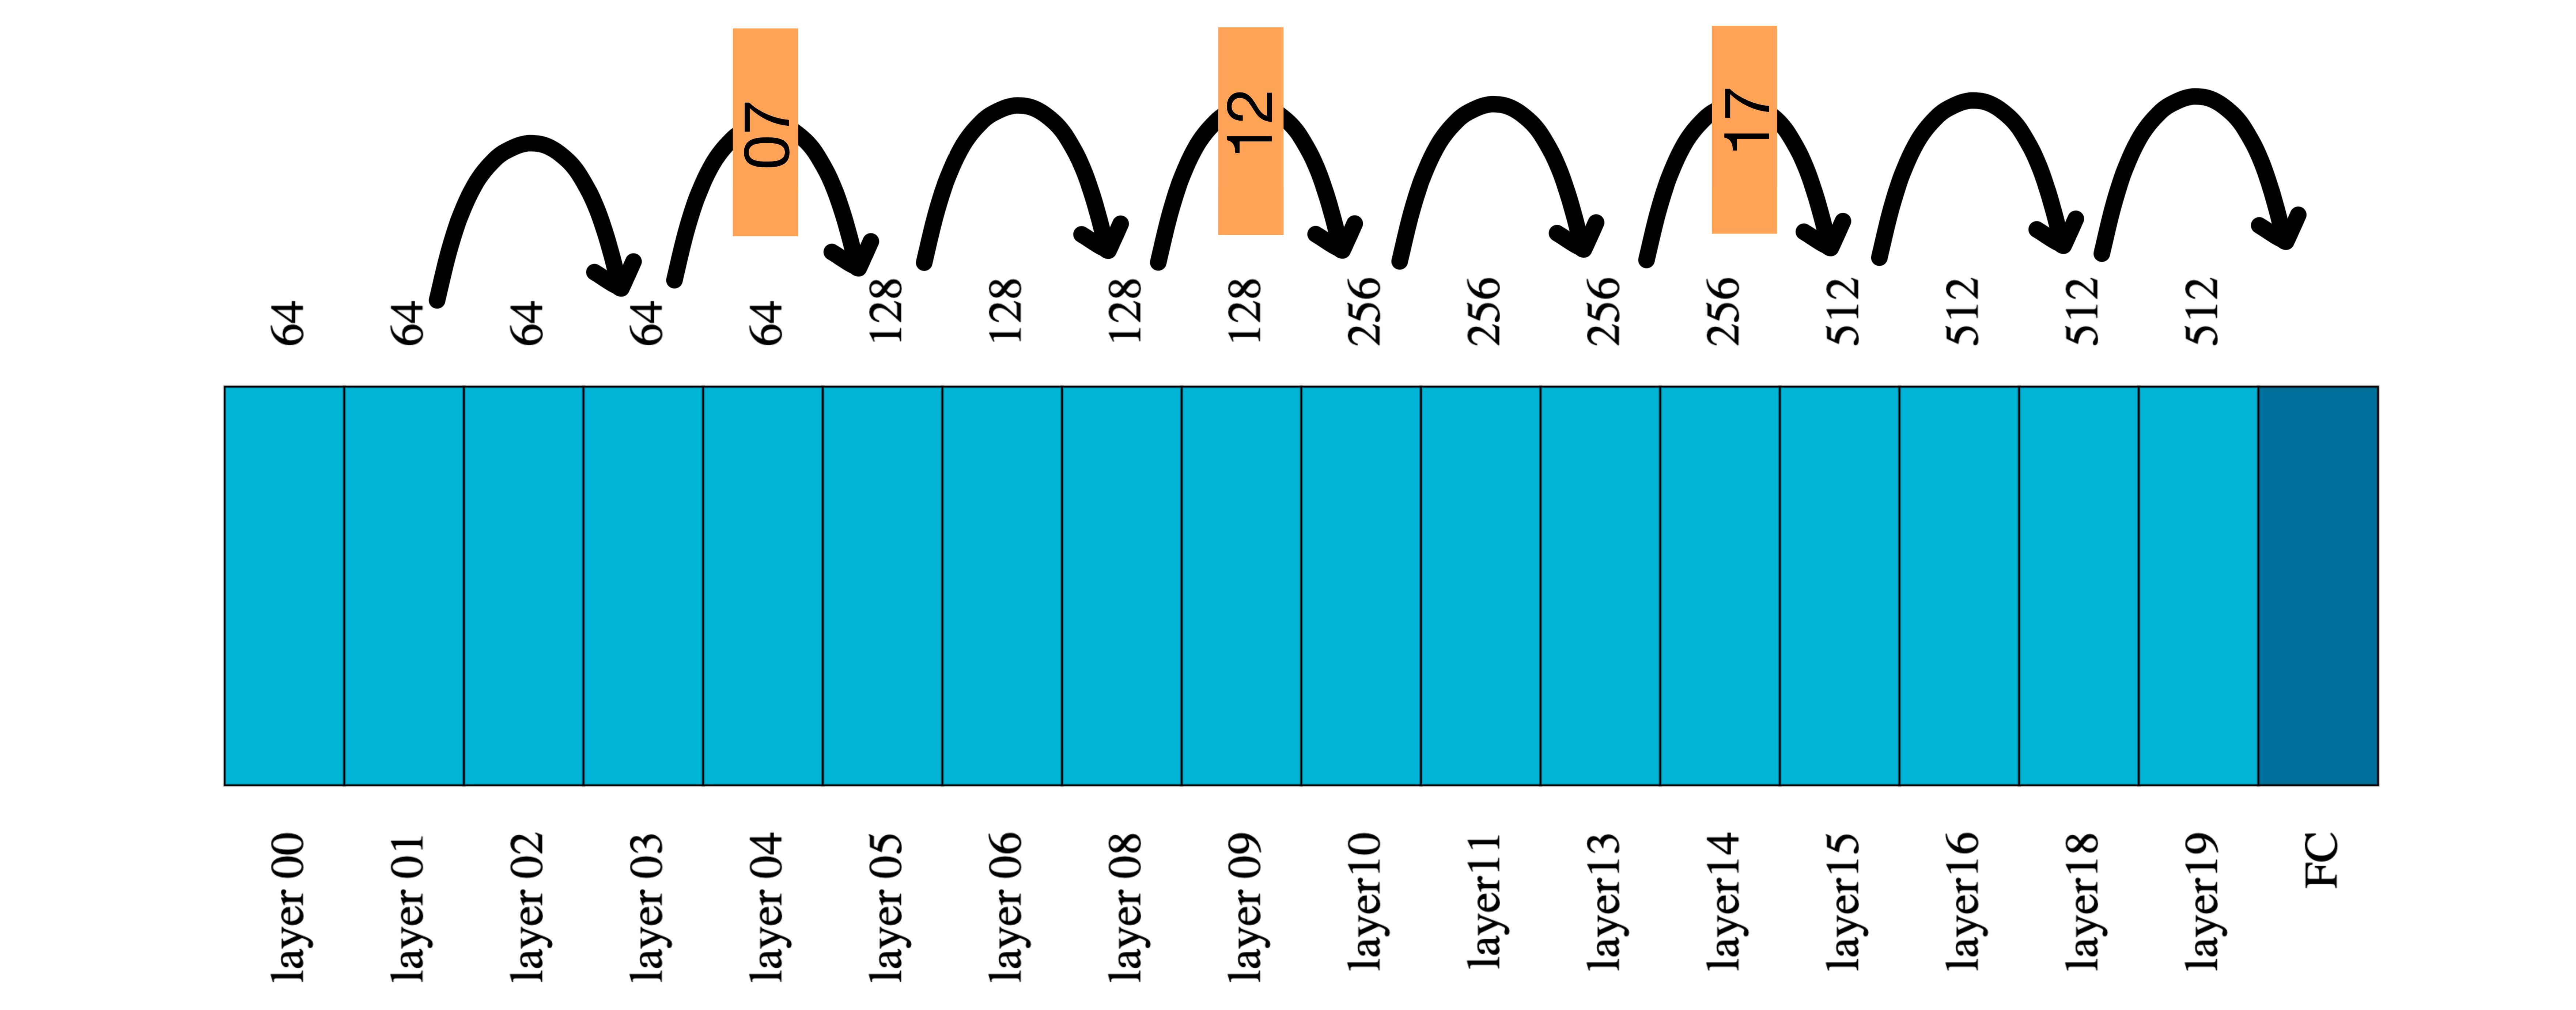
\includegraphics[width=0.96\columnwidth]{drawing}
\caption{ ResNet-18 architecture with layer indices of convolutional layers and the
number of filters in each layer. } \label{fig:resnet18} \end{figure}



\clearpage

\subsection{Plot of Figure \ref{fig:norm_plots}}
\label{sec:big_plots}


\begin{figure}[h]
\centering

\begin{subfigure}[t]{0.34\textwidth}
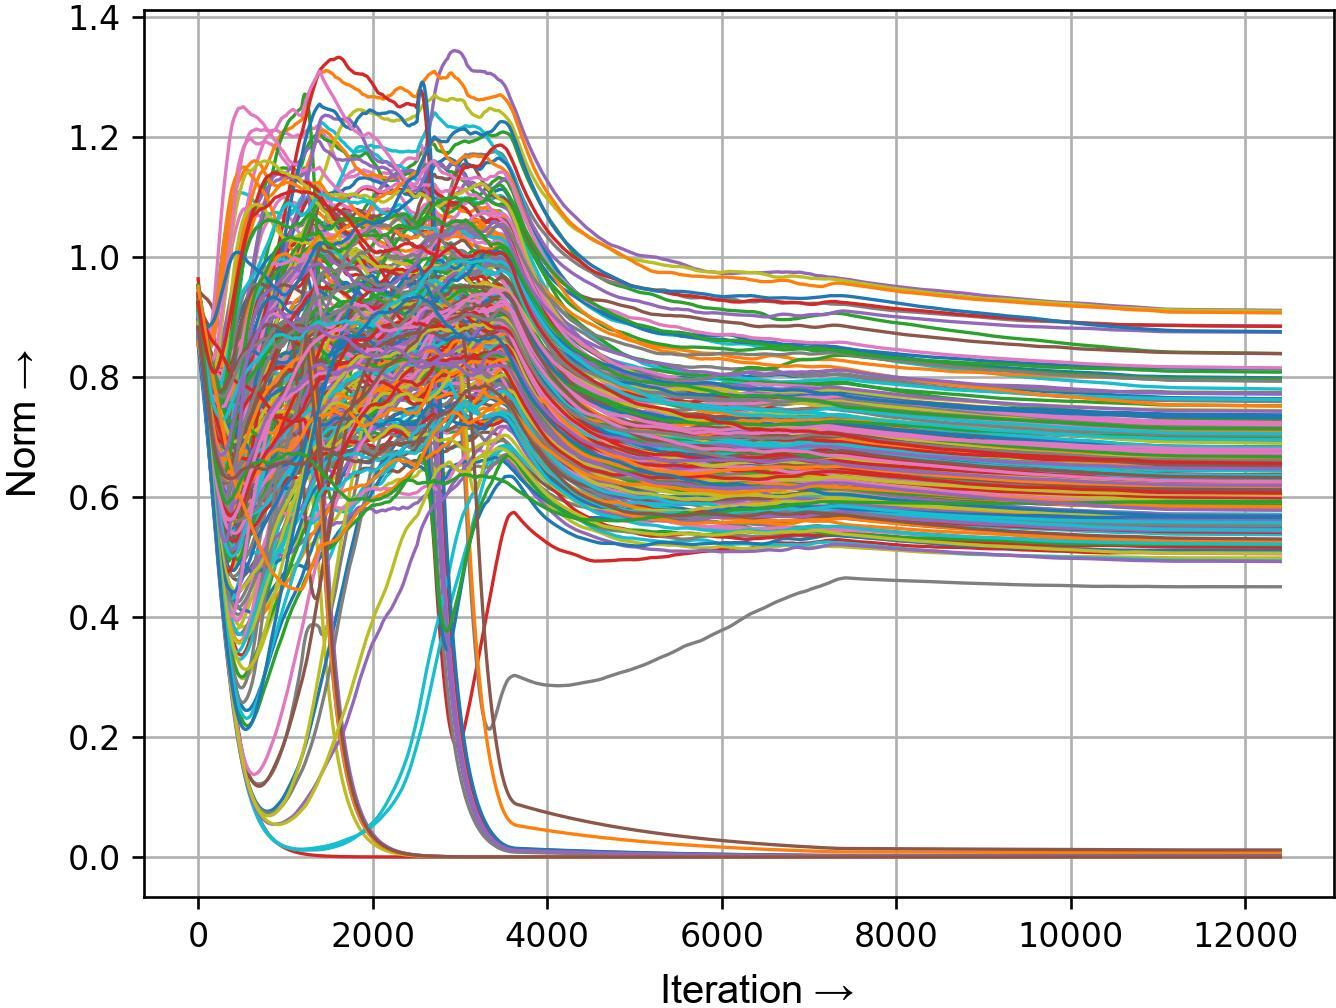
\includegraphics[width=\textwidth]{trimmed/baseline-w-layer-4-2}
\caption{Layer 11\\ \forceindentb\textbf{baseline}}
\end{subfigure}
\begin{subfigure}[t]{0.34\textwidth}
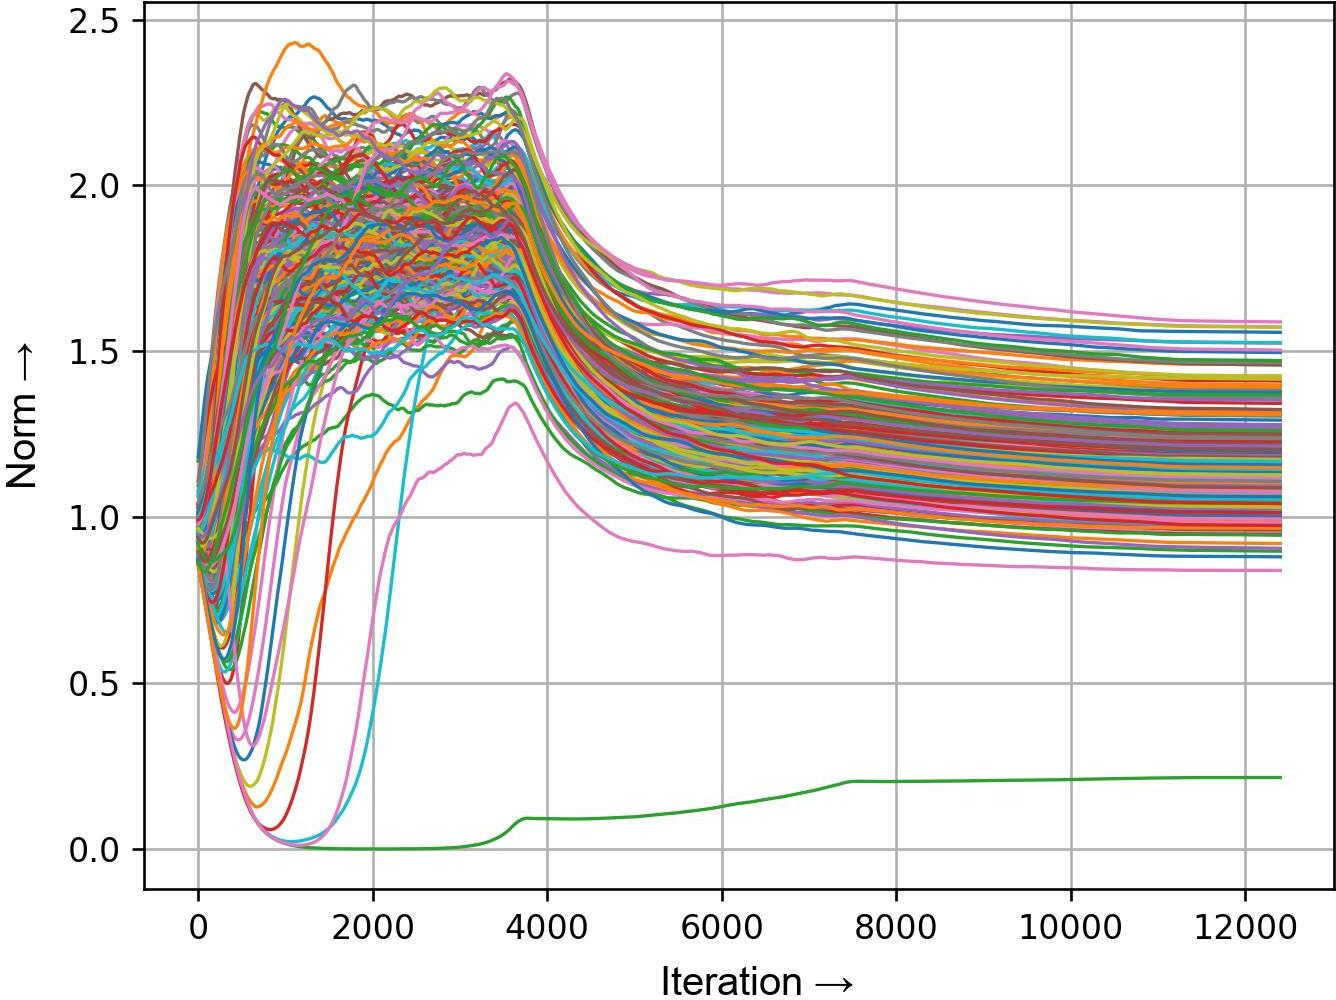
\includegraphics[width=\textwidth]{trimmed/pgt-w-layer-4-2}
\caption{Layer 11\\ \forceindentb\textbf{PGT}}
\end{subfigure}

\begin{subfigure}[t]{0.34\textwidth}
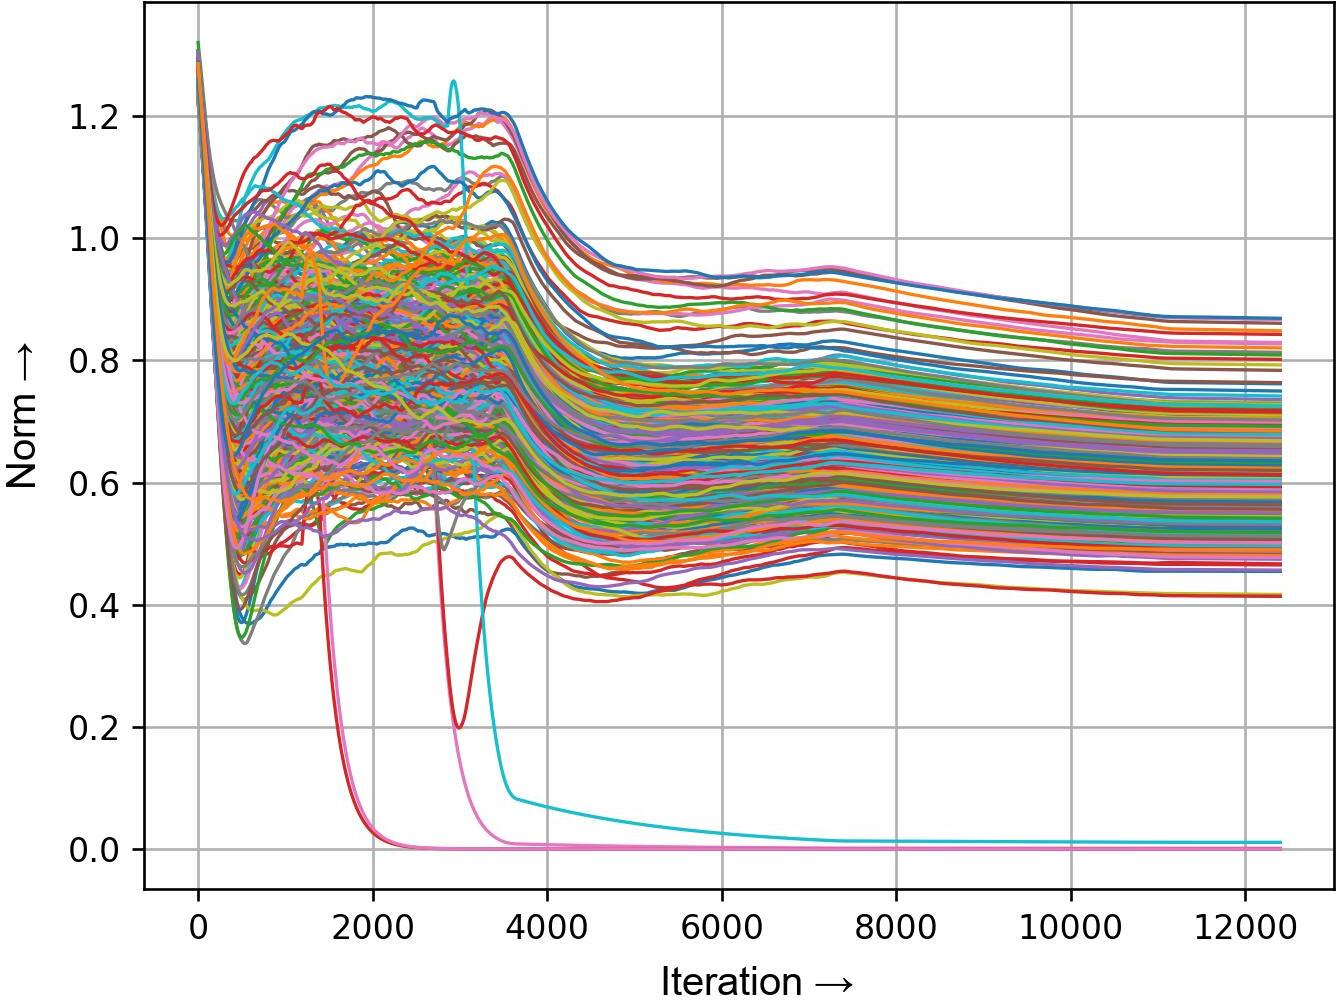
\includegraphics[width=\textwidth]{trimmed/baseline-w-layer-7-2}
\caption{Layer 19\\ \forceindentb\textbf{baseline}}
\end{subfigure}
\begin{subfigure}[t]{0.34\textwidth}
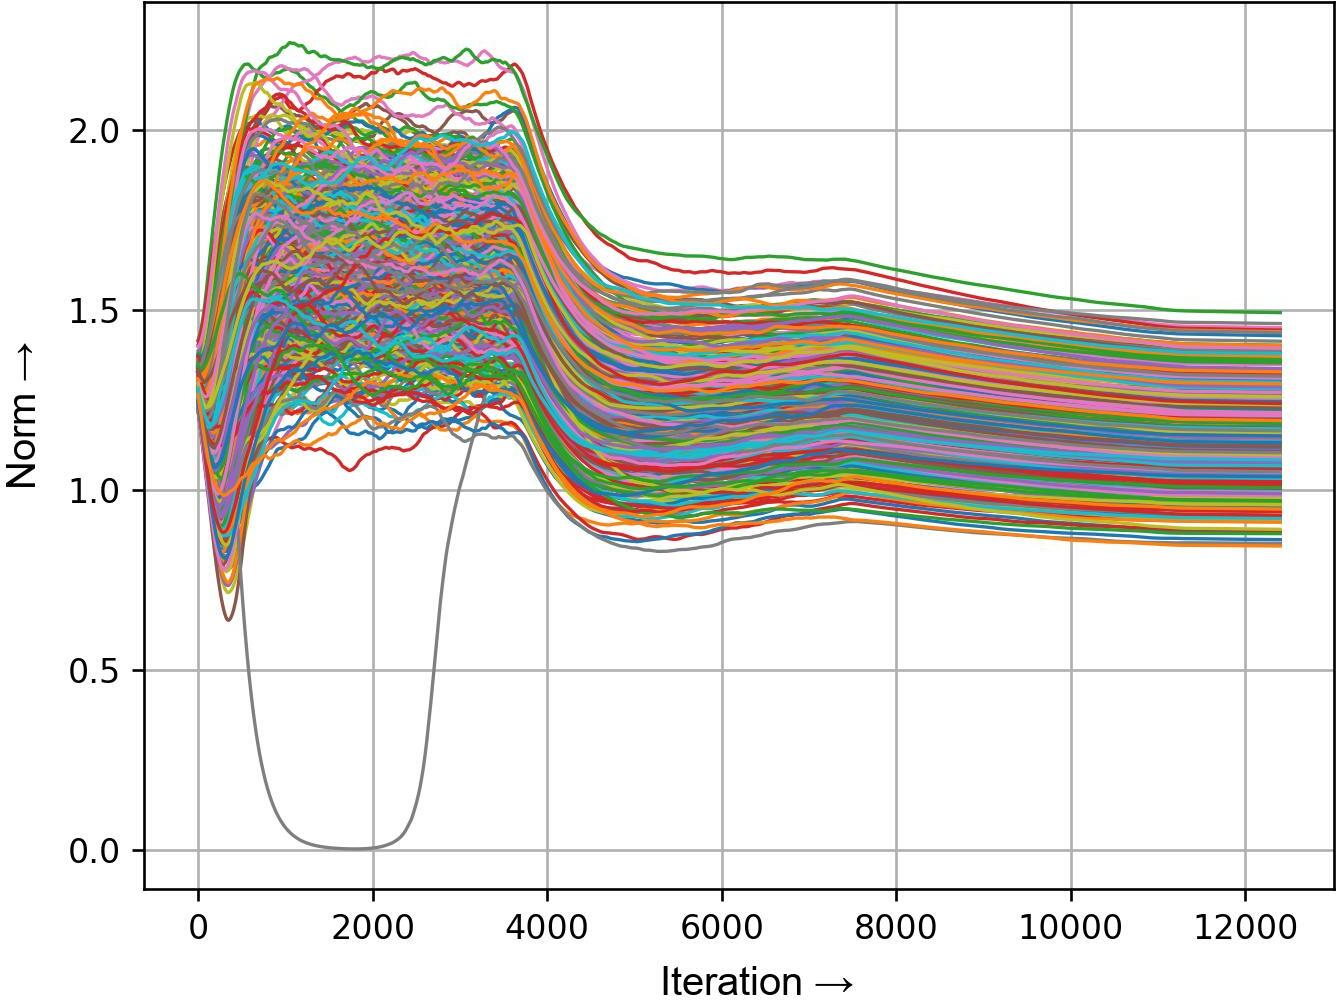
\includegraphics[width=\textwidth]{trimmed/pgt-w-layer-7-2}
\caption{Layer 19\\ \forceindentb\textbf{PGT}}
\end{subfigure}

\begin{subfigure}[t]{0.34\textwidth}
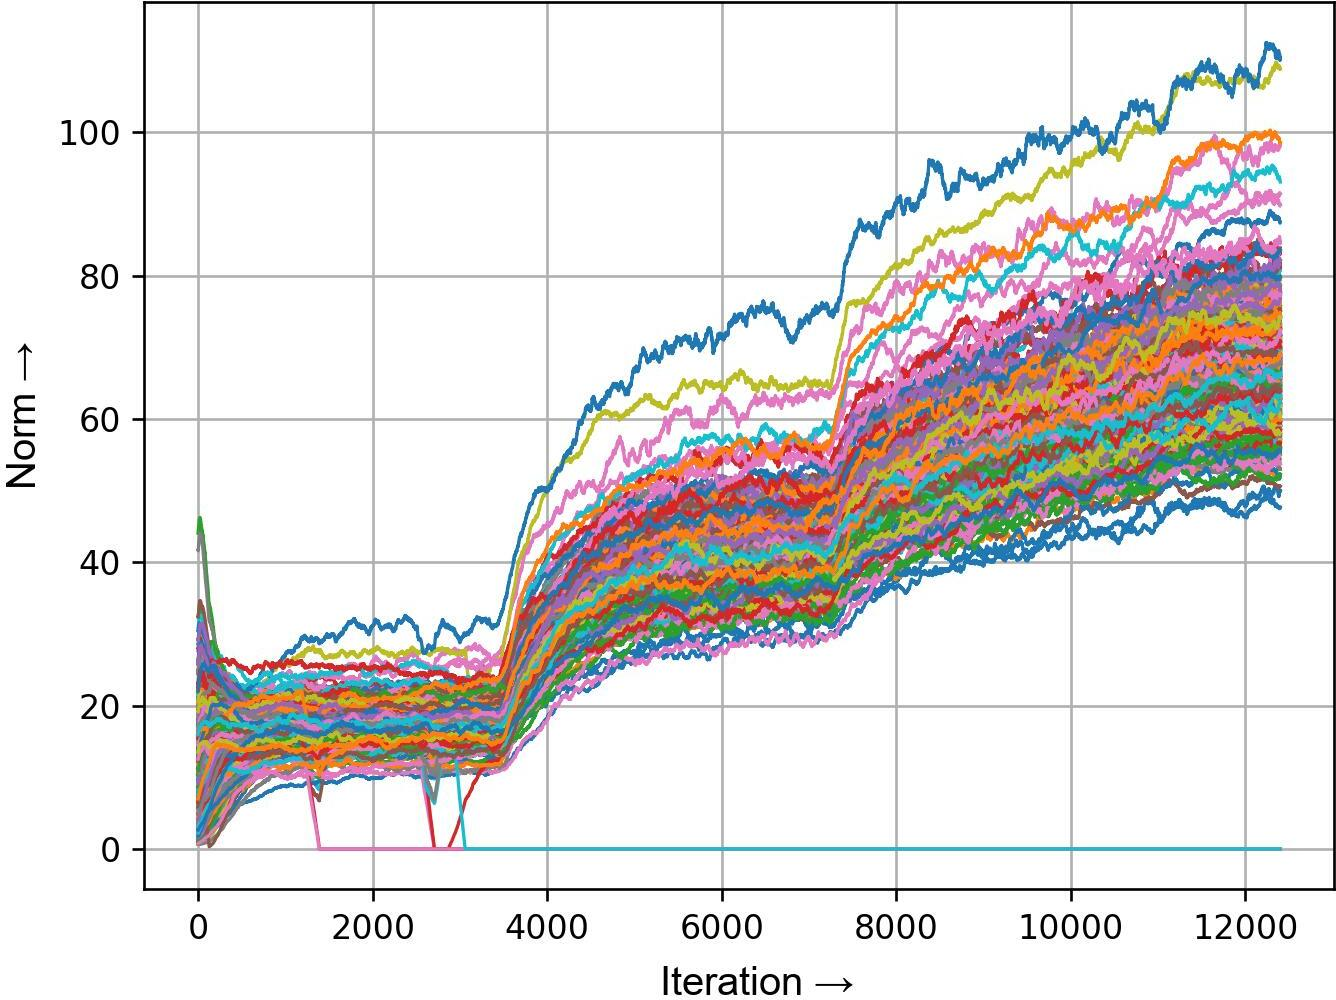
\includegraphics[width=\textwidth]{trimmed/baseline-f-layer-22-1}
\caption{GAP features\\ \forceindentb\textbf{baseline}}
\end{subfigure}
\begin{subfigure}[t]{0.34\textwidth}
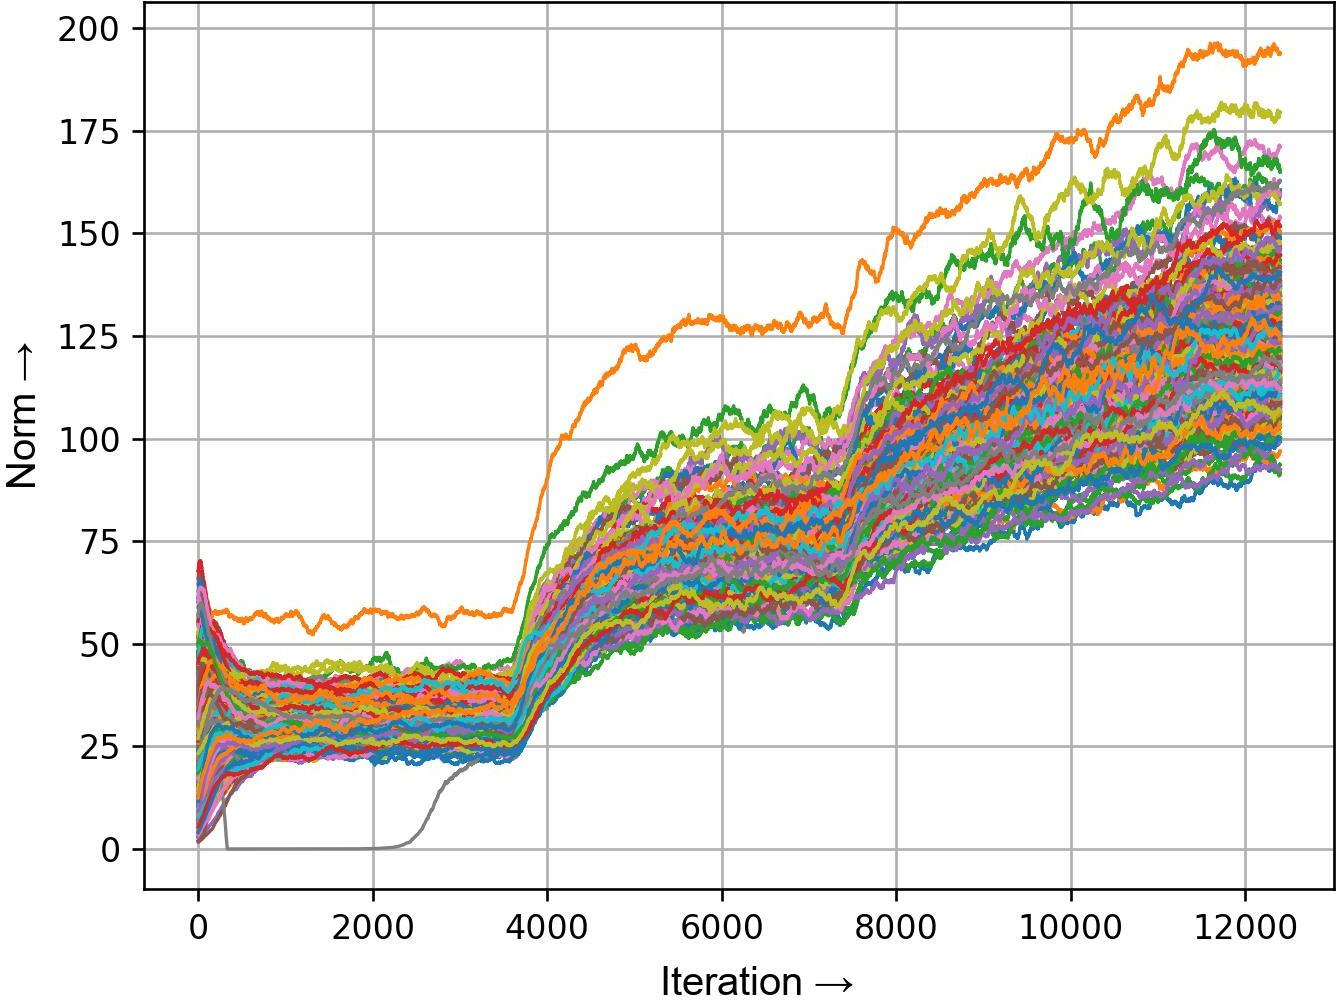
\includegraphics[width=\textwidth]{trimmed/pgt-f-layer-22-1}
\caption{GAP features\\ \forceindentb\textbf{PGT}}
\end{subfigure}
\caption{ Norm vs iter. plots demonstrating layer characteristics (the zero out
phenomena). Each colour represents a different filter or feature vector of a particular
layer of a non-BN variant of ResNet-18. }
\end{figure}

\clearpage


\begin{figure}[h]
\centering

\begin{subfigure}[t]{0.34\textwidth}
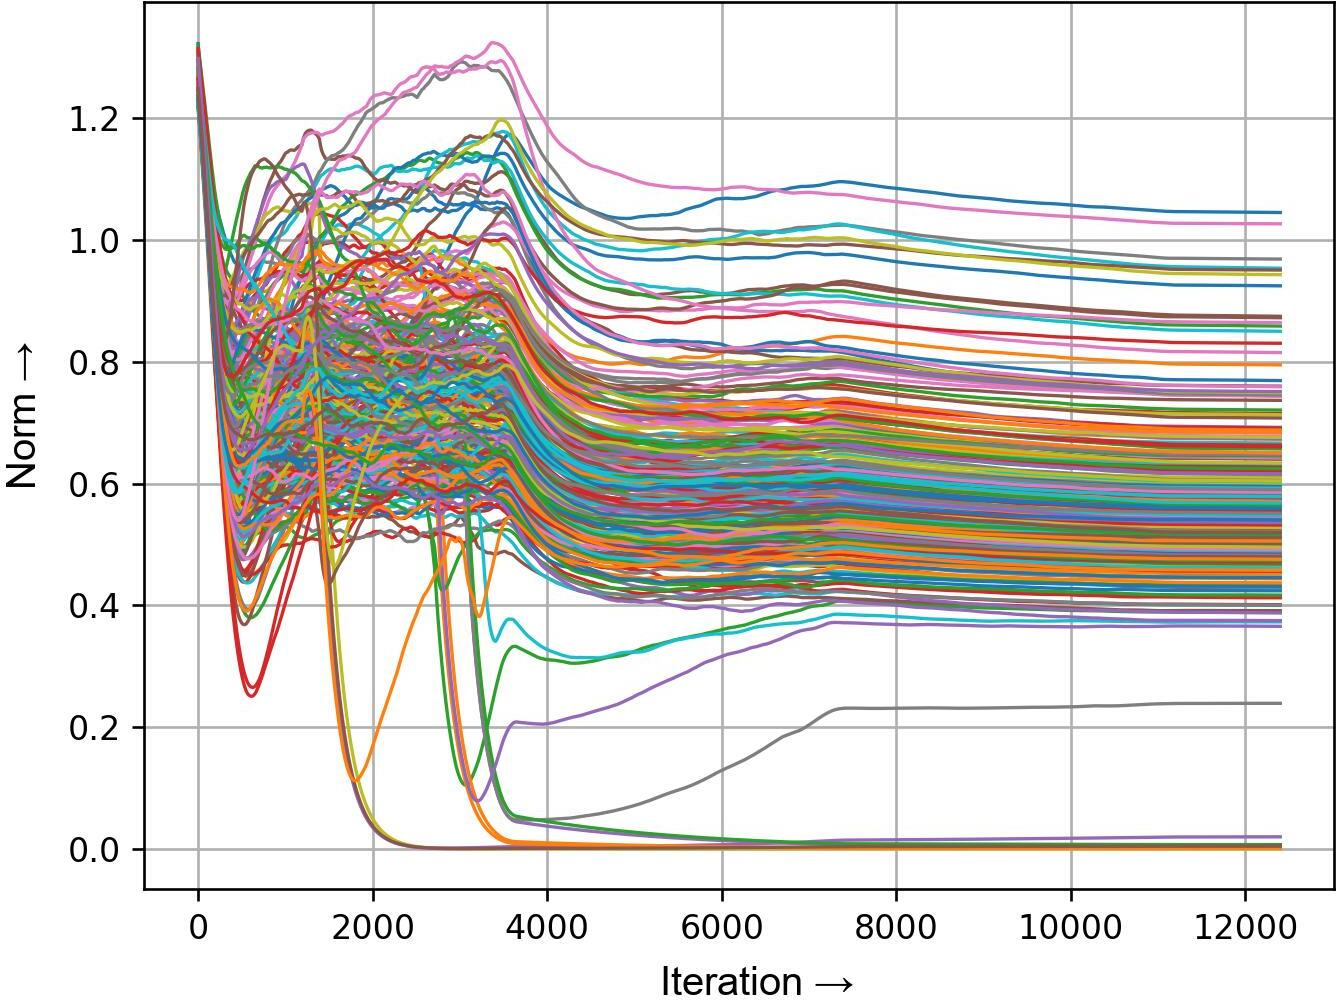
\includegraphics[width=\textwidth]{trimmed/baseline-w-layer-5-3}
\caption{Layer 15\\ \forceindentb\textbf{baseline}}
\end{subfigure}
\begin{subfigure}[t]{0.34\textwidth}
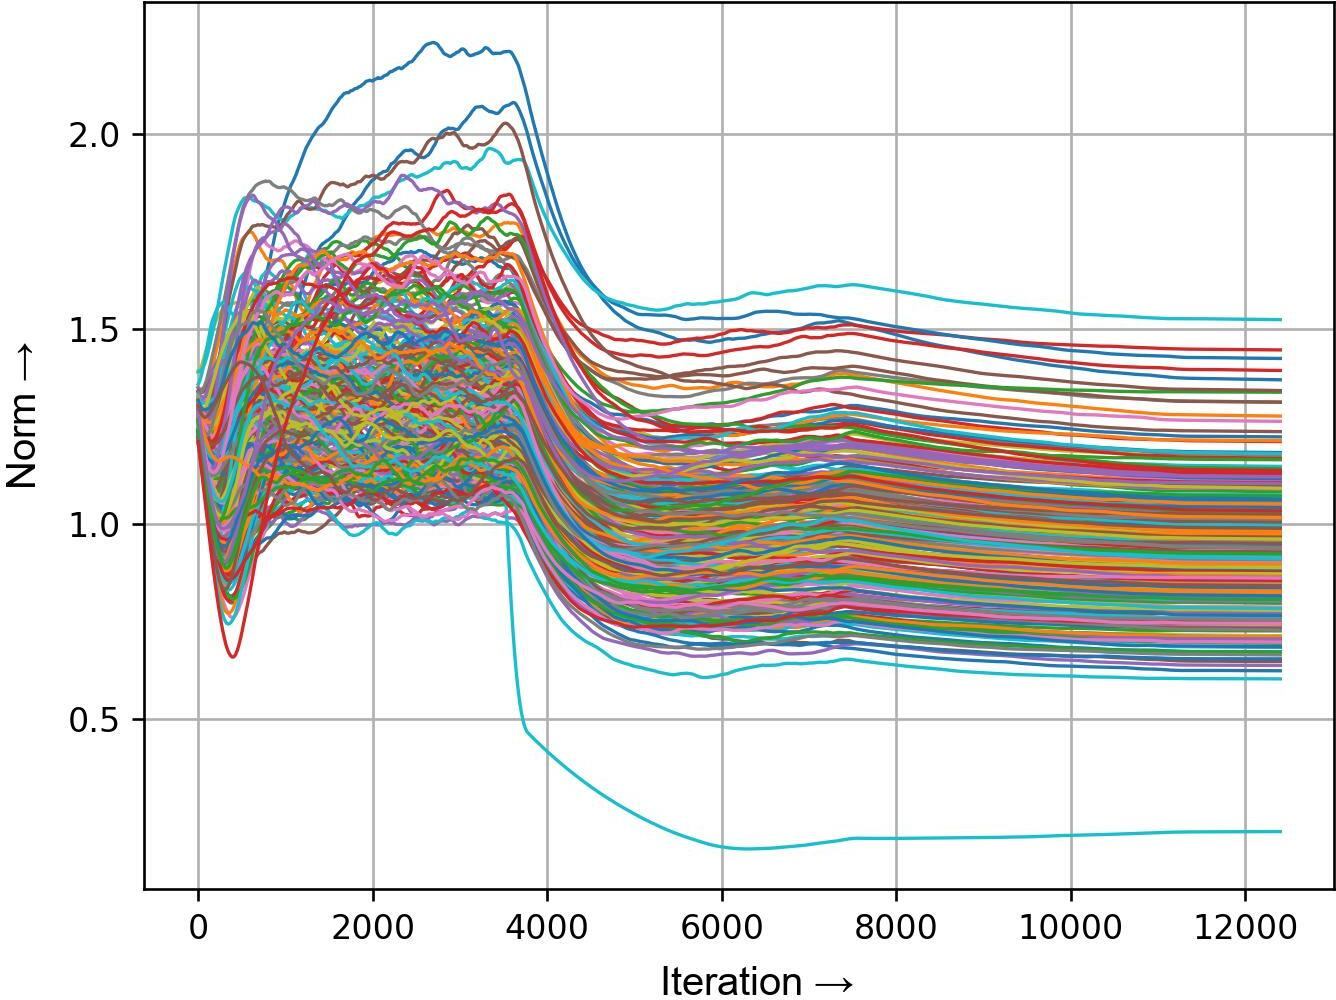
\includegraphics[width=\textwidth]{trimmed/pgt-w-layer-5-3}
\caption{Layer 15\\ \forceindentb\textbf{PGT}}
\end{subfigure}

\begin{subfigure}[t]{0.34\textwidth}
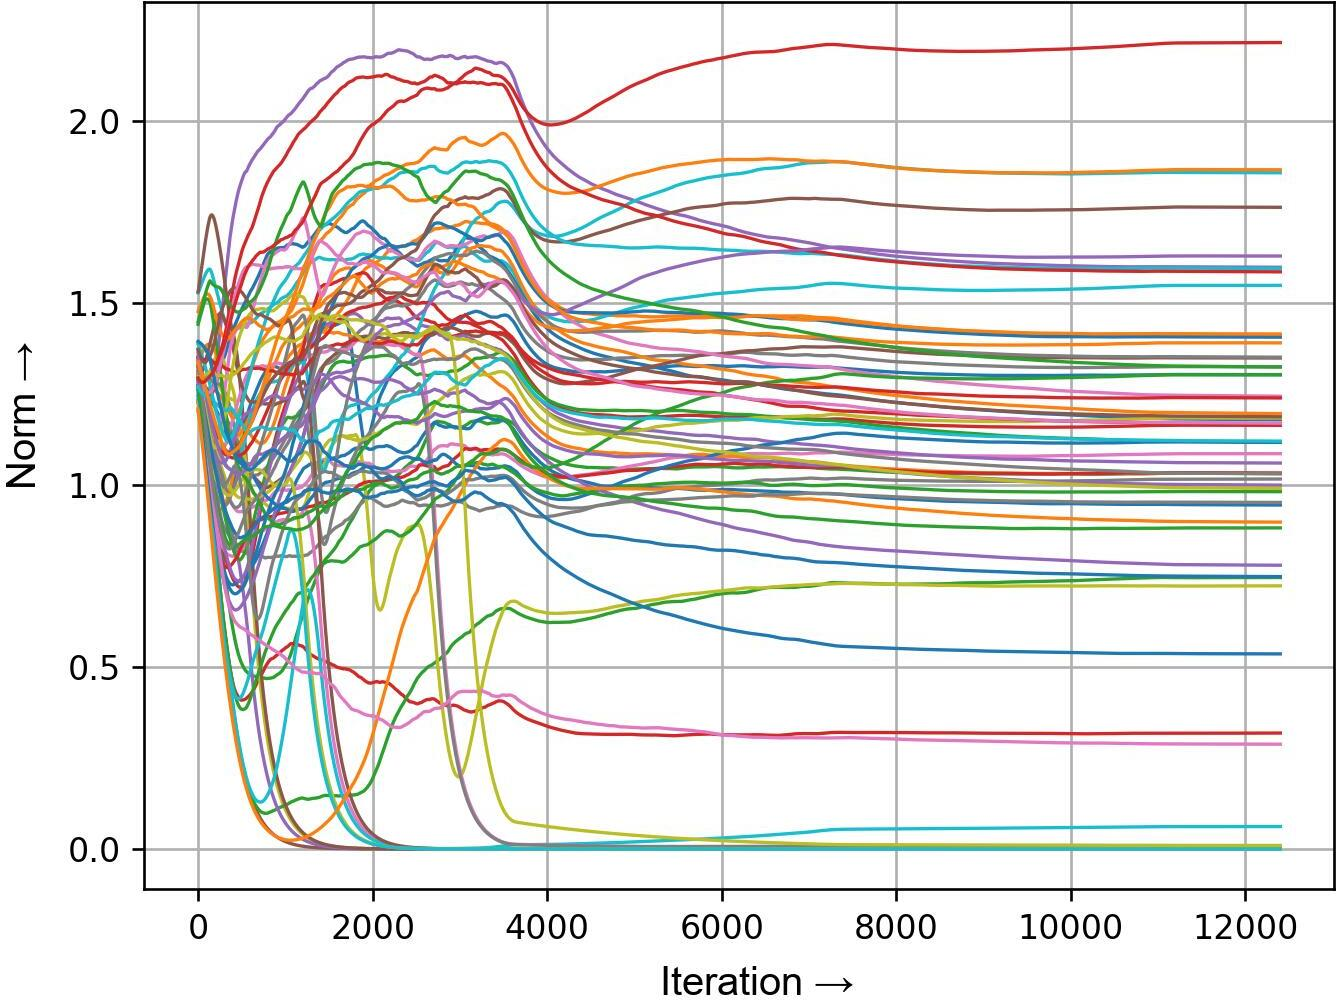
\includegraphics[width=\textwidth]{trimmed/baseline-w-layer-1-2}
\caption{Layer 2\\ \forceindentb\textbf{baseline}}
\end{subfigure}
\begin{subfigure}[t]{0.34\textwidth}
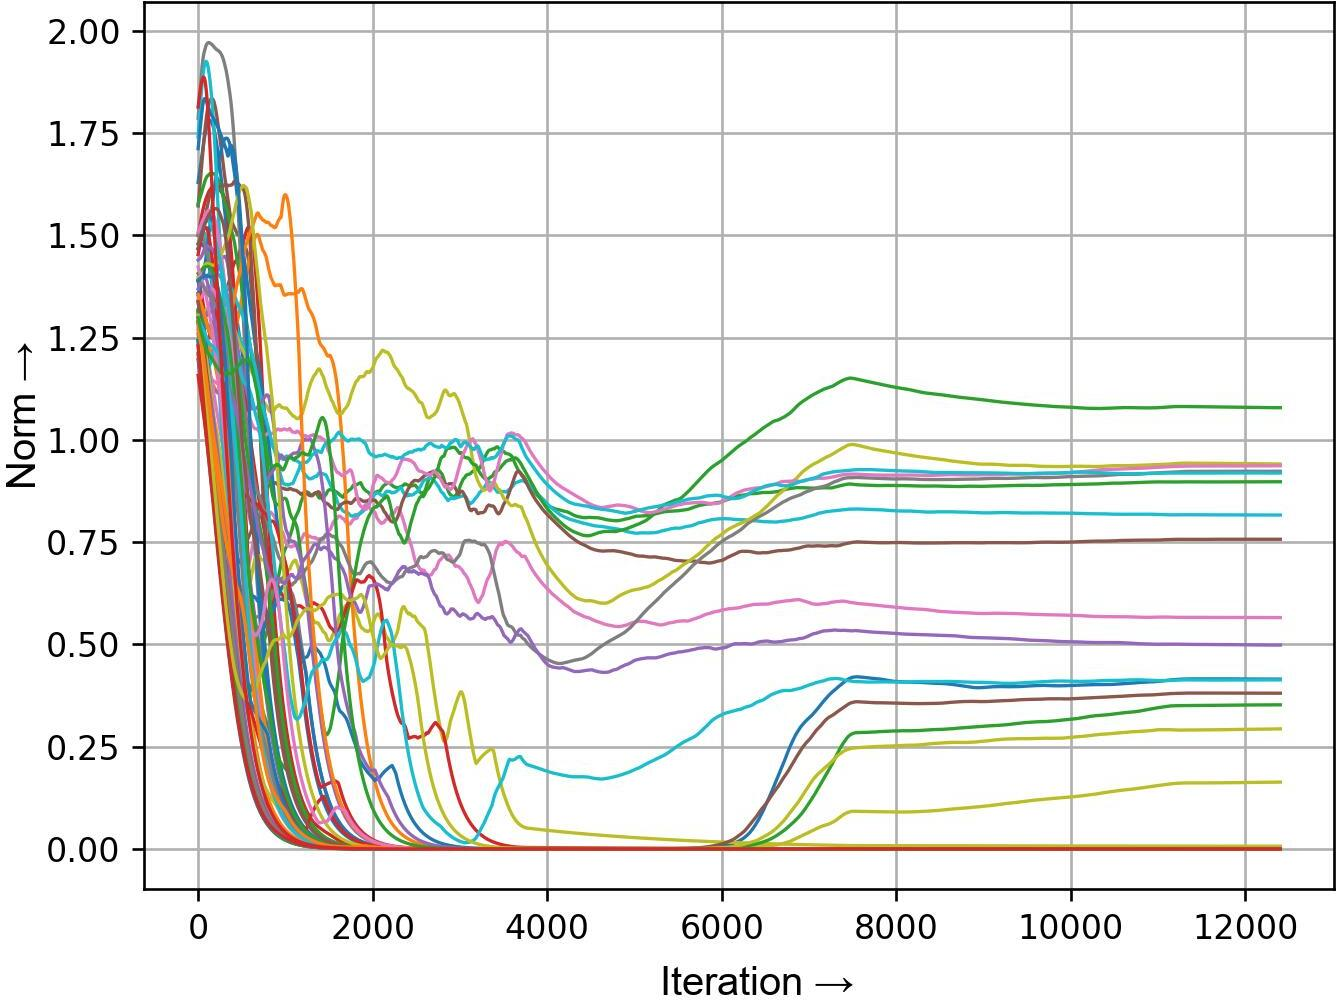
\includegraphics[width=\textwidth]{trimmed/pgt-w-layer-1-2}
\caption{Layer 2\\ \forceindentb\textbf{PGT}}
\end{subfigure}

\begin{subfigure}[t]{0.34\textwidth}
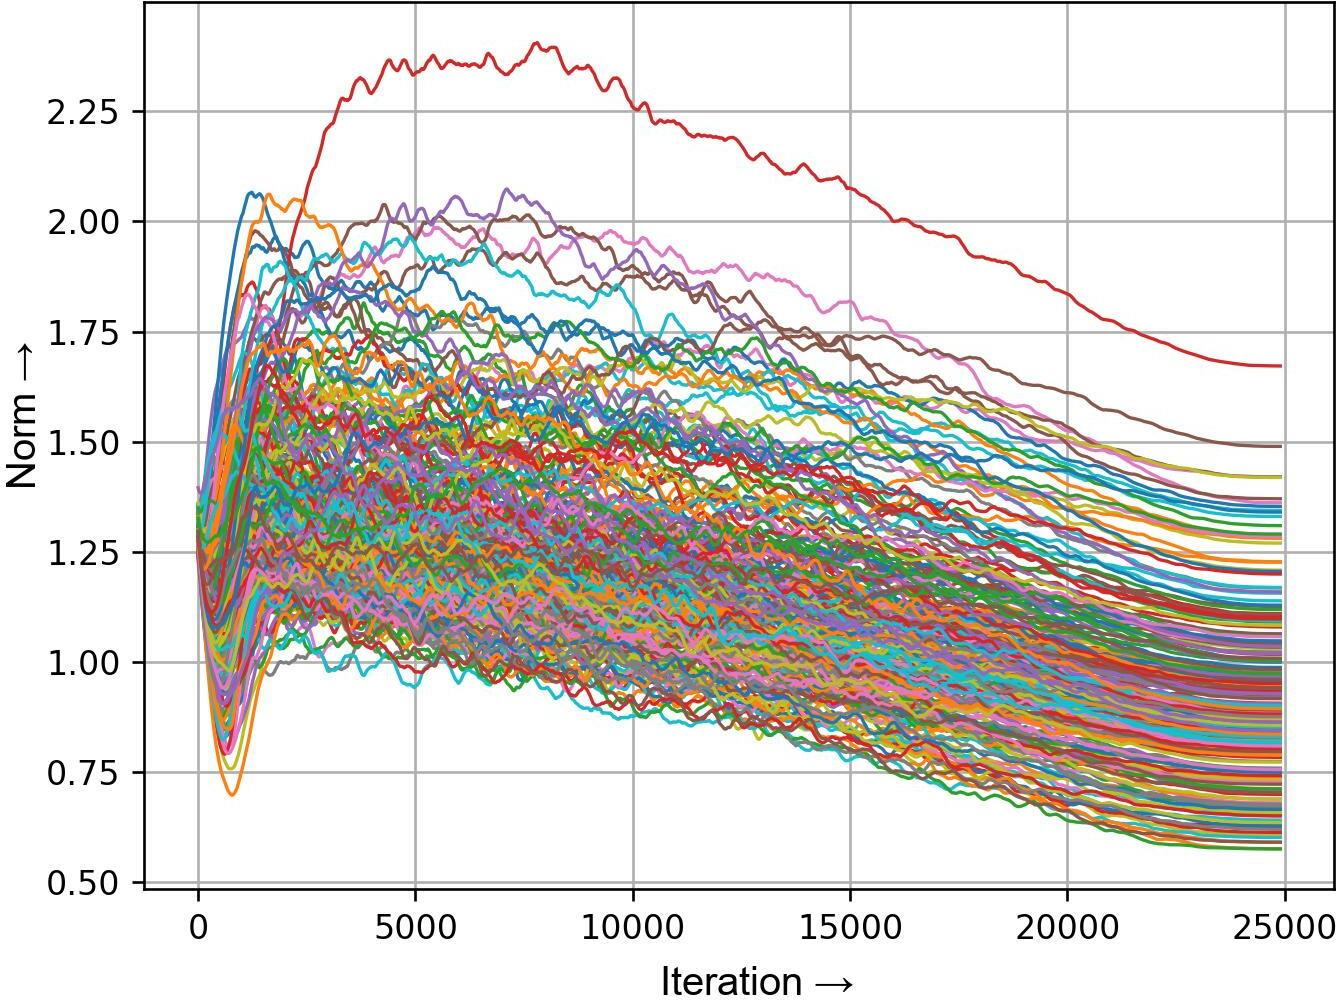
\includegraphics[width=\textwidth]{trimmed/agc_pgt-w-layer-5-3}
\caption{Layer 15\\ \forceindenta\textbf{AGC+PGT}}
\end{subfigure}
\begin{subfigure}[t]{0.34\textwidth}
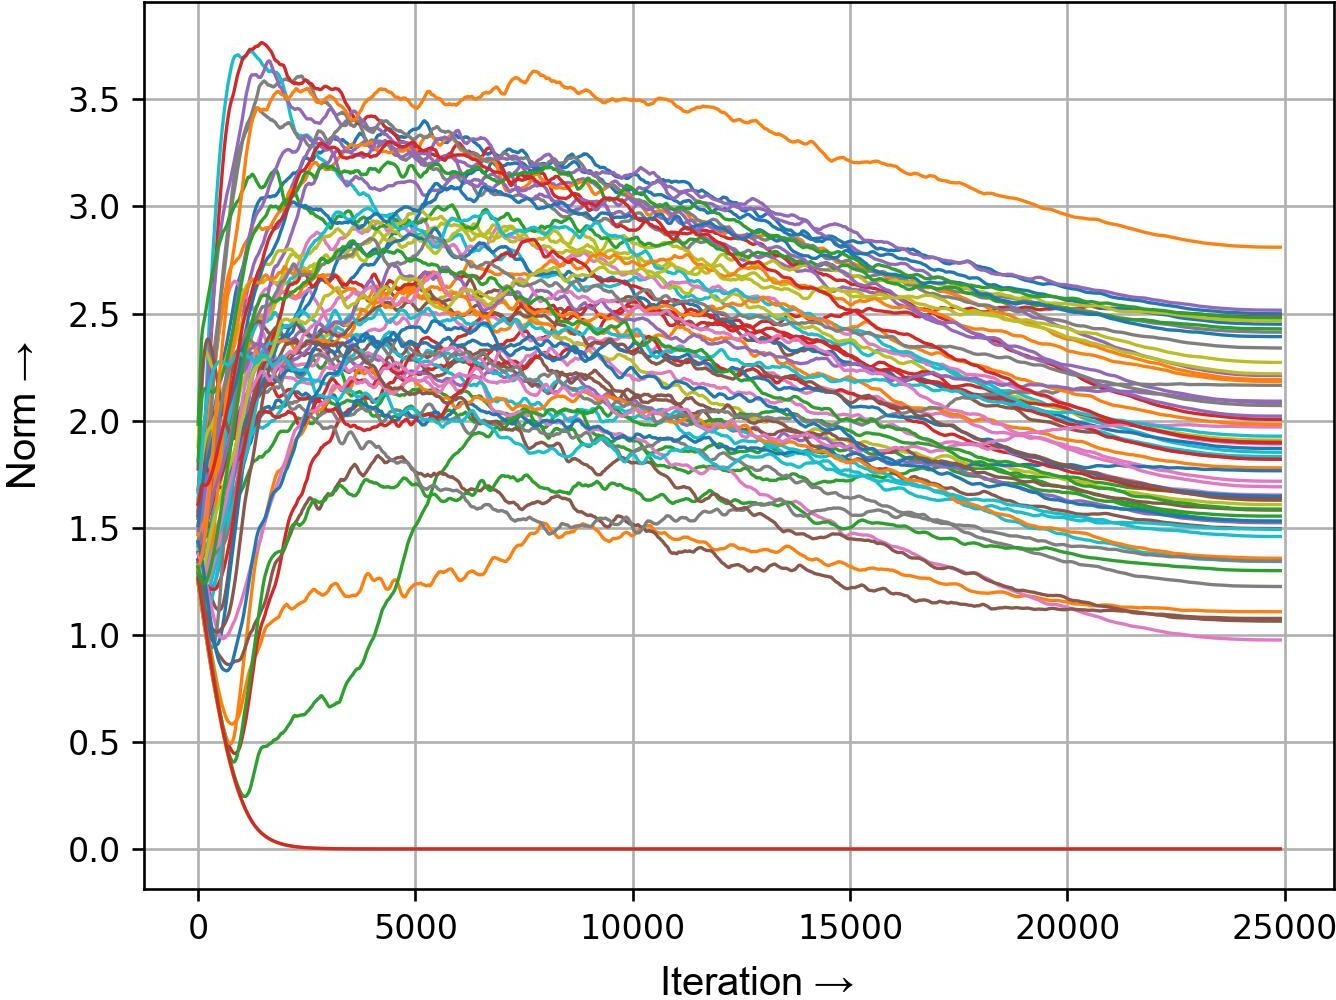
\includegraphics[width=\textwidth]{trimmed/agc_pgt-w-layer-1-2}
\caption{Layer 2\\ \forceindenta\textbf{AGC+PGT}}
\end{subfigure}
\caption{ Norm vs iter. plots demonstrating the efficacy of PGT and AGC+PGT over
baseline. Each colour represents a different filter or feature vector of a particular
layer of a non-BN variant of ResNet-18. }
\end{figure}

\end{document}
